\documentclass[preprint,12pt]{elsarticle}
% Extended revision and answer question (2 reviewers)
% for JPM-1174473
%Since April 19, 2021
%Please resubmit your revised manuscript through the following link:
% https://susy.mdpi.com/user/manuscripts/upload?pre_hash_key=6f6b5248032093559a0cdfda5026f51f

\newenvironment{MyIndent}
{\par\leftskip1cm\relax\rightskip1cm\relax}
{\par\leftskip0cm\relax\rightskip0cm\relax}

%\usepackage{xr}  % for cross-reference
\usepackage{xr-hyper}
\usepackage{hyperref}

%\newcommand{\R}[1]{\label{#1}\linelabel{#1}} % for \label page and line
%\newcommand{\lr}[1]{page~\pageref{#1} (line~\lineref{#1})} % for \ref page and line
\makeatletter
  \long\def\myempty{}
  \def\XR@addURL#1{\XR@@dURL#1\myempty{}{}{}{}{}\\}
  \def\XR@@dURL#1#2#3#4#5#6#7\\{%
    {#1}{#2}%
    \ifx\myempty#6\@empty
      {#3}{#4}{\XR@URL}%
    \else
    \fi
  }
\makeatother

\makeatletter
\newcommand*{\addFileDependency}[1]{% argument=file name and extension
  \typeout{(#1)}
  \@addtofilelist{#1}
  \IfFileExists{#1}{}{\typeout{No file #1.}}
}
\makeatother

\newcommand*{\myexternaldocument}[1]{%
    \externaldocument{#1}%
    \addFileDependency{#1.tex}%
    \addFileDependency{#1.aux}%
}
% turn it off
%\myexternaldocument{main} % or main_REDmarked_revision2.tex
%\externaldocument{main}

\usepackage{tikz-imagelabels} % for  tikz
\usepackage{siunitx} % for  1e-10 scientific notation
\usepackage[bf]{caption}
\newcommand{\bcaption}[2]{\caption{\textbf{#1} #2}}

\usepackage{subcaption} % for figure  side by side

% mark in blue or red
\usepackage{xcolor}
\definecolor{asparagus}{rgb}{0.53, 0.66, 0.42}
%\usepackage[table,xcdraw]{xcolor}
\newenvironment{MyColorPar}[1]{%
    \leavevmode\color{#1}\ignorespaces%
}{%
}%

\usepackage{outlines}

%%% for abbreviations, or acronyms
\usepackage[acronym, nopostdot]{glossaries} 
%\usepackage{glossary-inline}
%\newenvironment{abbreviation}
%\makeglossaries %https://tex.stackexchange.com/questions/110095/list-of-acronyms-is-not-displayed
\newacronym{ncbi}{NCBI}{National Center for Biotechnology Information}
\newacronym{degs}{DEGs}{differentially expressed genes}

\newacronym{fdr}{FDR}{false discovery rate}
\newacronym{hpa}{HPA}{the Human Protein Atlas}
\newacronym{hnscc}{HNSCC}{head and neck squamous cell carcinoma}
\newacronym{tcga}{TCGA}{the Cancer Genome Atlas}
\newacronym{tcpa}{TCPA}{the Cancer Proteome Atlas}
\newacronym{rna}{RNA}{ribonucleic acid}
\newacronym{rnaseq}{RNA-Seq}{RNA sequencing}
\newacronym{lncrna}{lncRNA}{long non-coding RNA}
%\newacronym{km}{KM}{Kaplan-Meier}
\newacronym{rppa}{RPPAs}{reverse-phase protein arrays}
\newacronym{rpma}{RPMA}{reverse-phase protein lysate microarray}

\newacronym{mmp}{MMP}{matrix metalloproteinase}
 %DKK1, CAMK2N1, STC2, PGK1, SURF4, USP10, NDFIP1, FOXA2, STIP1, and DKC1
 %ZNF557, ZNF266, IL19, MYO1H, FCGBP, LOC148709, EVPLL, PNMA5, KIAA1683, and NPB

\newacronym{DKK1}{DKK1}{dickkopf WNT signaling pathway inhibitor 1} 
\newacronym{CAMK2N1}{CAMK2N1}{calcium/calmodulin dependent protein kinase II inhibitor 1} 
\newacronym{CALML5}{CALML5}{calmodulin like 5}

\newacronym{STC2}{STC2}{stanniocalcin 2} 
\newacronym{PGK1}{PGK1}{phosphoglycerate kinase 1} 
\newacronym{SURF4}{SURF4}{surfeit 4} 
\newacronym{USP10}{USP10}{ubiquitin specific peptidase 10} 
\newacronym{NEDD4}{NEDD4}{neural precursor cell expressed, developmentally down-regulated 4}
\newacronym{NDFIP1}{NDFIP1}{NEDD4 family interacting protein 1} 
\newacronym{FOXA2}{FOXA2}{forkhead box A2} 
\newacronym{STIP1}{STIP1}{stress-induced-phosphoprotein 1} 
\newacronym{DKC1}{DKC1}{dyskeratosis congenita 1, dyskerin} 

\newacronym{ZNF557}{ZNF557}{zinc finger protein 557} 
\newacronym{ZNF266}{ZNF266}{zinc finger protein 266} 
\newacronym{IL19}{IL19}{interleukin 19} 
\newacronym{MYO1H}{MYO1H}{myosin 1H} 
\newacronym{FCGBP}{FCGBP}{Fc fragment of IgG binding protein} 
\newacronym{LOC148709}{LOC148709}{LncRNA LOC148709} 
\newacronym{EVPLL}{EVPLL}{envoplakin-like protein} 
\newacronym{PNMA5}{PNMA5}{paraneoplastic antigen like 5} 
%\newacronym{KIAA1683}{KIAA1683}{IQCN, IQ Motif Containing N} 
\newacronym{IQCN}{IQCN}{IQ motif containing N} % previous name KIAA1683
% "IQ" refers to the first two amino acids of the motif: isoleucine (commonly) and glutamine (invariably)
\newacronym{NPB}{NPB}{neuropeptide B} 

 \newacronym{rt}{RT}{radiation therapy}
 \newacronym{nccn}{NCCN}{National Comprehensive Cancer Network}
 \newacronym{hif}{HIF}{hypoxia-inducible factor}
 \newacronym{egfr}{EGFR}{epidermal growth factor receptor}
 \newacronym{ras}{RAS}{rat sarcoma}
 \newacronym{hras}{HRAS}{Harvey rat sarcoma viral oncoprotein}
 \newacronym{erk}{ERK}{extracellular signal-regulated kinases}
 \newacronym{us}{US}{United States}
 \newacronym{fda}{FDA}{Food and Drug Administration}
 \newacronym{tpf}{Tax-PF}{docetaxel, cisplatin, and 5-fluorouracil}
 \newacronym{tki}{TKI}{tyrosine kinase inhibitor}
 \newacronym{her}{HER}{human epidermal growth factor receptor}
 \newacronym{ici}{ICI}{immune-checkpoint inhibitor}
 \newacronym{ctla4}{CTLA-4}{cytotoxic T lymphocyte antigen 4}
 \newacronym{pd1}{PD-1}{programmed death 1}
 \newacronym{pdl1}{PD-L1}{programmed death ligand 1}
 \newacronym{tim3}{TIM-3}{T-cell immunoglobulin mucin protein 3}
 \newacronym{lag3}{LAG-3}{lymphocyte activation gene 3}
 \newacronym{ifng}{IFN-$\gamma$}{interferon gamma}
 \newacronym{tigit}{TIGIT}{T cell immunoglobin and immunoreceptor tyrosine-based inhibitory motif}
 \newacronym{gitr}{GITR}{glucocorticoid-induced tumor necrosis factor receptor}
 \newacronym{vista}{VISTA}{V-domain Ig suppressor of T-cell activation}
 \newacronym{tmsb4x}{TMSB4X}{thymosin beta-4 X-linked}
 \newacronym{emt}{EMT}{epithelial-mesenchymal-transition}
 \newacronym{gdc}{GDC}{Genomic Data Commons}
 \newacronym{nci}{NCI}{the National Cancer Institute}
 \newacronym{gdac}{GDAC}{Genome Data Analysis Center}
 \newacronym{rest}{REST}{Representational State Transfer} 
 \newacronym{api}{API}{Application Programmable Interface}
\newacronym{grch38}{GRCh38}{Genome Reference Consortium Homo sapiens genome assembly 38}
\newacronym{fpkm}{FPKM}{Fragments per kilobase per million reads mapped}
\newacronym{rsem}{RSEM}{RNA-Seq by Expectation-Maximization}
\newacronym{slca}{SLC35E2A}{solute carrier family 35 member E2A}
\newacronym{slcb}{SLC35E2B}{solute carrier family 35 member E2B}
\newacronym{cde}{CDE}{Common Data Element}
\newacronym{id}{ID}{identification}
\newacronym{ajcc}{AJCC}{the American Joint Committee on Cancer}
\newacronym{uicc}{UICC}{he Union for International Cancer Control}
\newacronym{tnm}{TNM}{the tumor size (T), cervical lymph node metastases (N), and distal metastasis status (M)}
\newacronym{ci95}{95\% CI}{95\% confidence interval}
\newacronym{os}{OS}{overall survival}
\newacronym{hr}{HR}{hazard ratio}
\newacronym{hpv}{HPV}{human papillomavirus}
\newacronym{ene}{ENE}{extra-nodal extension}
\newacronym{lvsi}{LVSI}{lymph-vascular space invasion}
\newacronym{pni}{PNI}{perineural invasion}
\newacronym{doi}{DOI}{depth of invasion}
\newacronym{lnd}{LND}{lymph node density}
\newacronym{wpoi5}{WPOI-5}{worst pattern of invasion score 5}
\newacronym{glut4}{GLUT4}{glucose transporters 4}
\newacronym{slc2a4}{SLC2A4}{solute carrier family 2 member A4}
\newacronym{trim24}{TRIM24}{tripartite motif-containing 24}
\newacronym{til}{TIL}{tumor-infiltrating lymphocytes}
\newacronym{tmb}{TMB}{tumor mutational burden}



%==================
\begin{document}

\section*{Cover letter for the re-submission (jpm-1174473)} 
% 2021/04/25
% 直接 online 填寫即可
%Please provide a cover letter to explain point-by-point the details of the revisions [changes 摘要即可 from the rebuttal]  in the manuscript
 


%Assistant Editor
%Suite 305, Zhongjia Mansion, Building No.13, Taiyangyuan Community, Dazhongsi 
%East Road,
%Haidian District, Beijing 100190, China
%Email: sonia.sun@mdpi.com
Assistant Editor of JPM%\newline

June 30, 2021

Dear Ms. Sonia Sun:

Enclosed, please find our revised manuscript (jpm-1174473) entitled "Transcriptomic Analysis for Prognostic Value in Head and Neck Squamous Cell Carcinoma" by Chi et al., which we wish to be considered for publishing as a research article in Journal of Personalized Medicine. We appreciate your time serving as the editor handling this manuscript and thank the reviewers for their critical comments and suggestions on our manuscript.

We have since revised the manuscript accordingly to address their critical comments and suggestions in a point-by-point manner, 


%{% A SUMMARY
Reviewer 1: % {2-4}
%"Please shortly explain the TCGA database in the Introduction and summarize the advantages of its use."\\
We re-wrote the Introduction in detail according to the suggestion by reviewer \#2.
added new supplementary Figure S1, S2, and S3
Reviewer 2: % {3-1}
%"Are the conclusions supported by the results?
We provide more evidence by additional analysis of TCGA and GEO databases. Moreover, we reviewed literature that supports the prognostic impact of these candidate genes.
%, S2, S3, and Table S2. We also replaced Figure 3D and 4A with high magnitude images from the same slides. We transferred the original Figure 2 into supplementary Figure S1 
%to provide more evidence from the significant literature review.
%}

%According to the editor's comments, we have the manuscript checked for English grammar. %
We wish our revised manuscript could be satisfied and accepted for publication in Journal of Personalized Medicine. 
Thanks very much for the kind helps and the reviewers' critical comments.
%\\[0.4cm]
Kind regards,

Yu-Chuan (Jack) Li, M.D., Ph.D.

Graduate Institute of Biomedical Informatics, 
College of Medical Science and Technology,\\
Taipei Medical University,
Taipei, Taiwan

%2) [cancers-1082127_main_redMarked] 自動化 by latex: red marked on page xx line xx
%"Track Changes" function in latex => by latexdiff
%Some options, taken from the documentation, include:
%UNDERLINE—added text is wavy-underlined and blue, discarded text is struck out and red;
%CTRADITIONAL—added text is blue and set in sans-serif, and a red footnote is created for each discarded piece of text;
%TRADITIONAL—like CTRADITIONAL but without the use of colour;
%CFONT—added text is blue and set in sans-serif, and discarded text is red and very small size;
%FONTSTRIKE—added text is set in sans-serif, discarded text small and struck out;
%CHANGEBAR—added text is blue, and discarded text is red. Additionally, the changed text is marked with a bar in the margin.
%https://www.overleaf.com/learn/latex/Articles/Using_Latexdiff_For_Marking_Changes_To_Tex_Documents

\pagebreak

\section*{Response to Reviewer 1 Comments}
%Response to Referees} % rebuttal
We much appreciate the reviewers for their helpful suggestions and critical comments on our manuscript. The detailed point-by-point answer to the reviewer's comments are as follows (marked as \textcolor{blue}{blue}). 
Moreover, the revised portions in the manuscript are indicated in \textcolor{red}{red}.

Comments and Suggestions for Authors from the reviewer \#1:

This manuscript perhaps describes the biomarkers of head and neck SCC using several data-bases. They also describe the relationship between the expression level of each candidate biomarkers in their patients and other factors such as gender, age, margin, lymph-node metastasis and so on.
%=> RNA expression and other contributing factors in the survival of HNSCC patients

I myself think this manuscript is very interesting, however, I do not find the difference between the previously published manuscript from your institute.
https://www.researchsquare.com/article/rs-80673/v1

\subsection*{1-1}
%\begin{MyColorPar}{blue}
%(OK)
First of all, please describe the difference between the two manuscripts.

%The authors have described the effectiveness of RNA sequencing as a tool for exploring prognostic factors; they have also performed a large-scale analysis using the TCGA cohort, which is a very attractive analysis method. I have a few minor questions.

%This is an attractive analysis method and I would like to know more details.

%It is generally known that high expression of EGFR is a poor prognostic factor in head and neck cancers, however, why is it that RNA sequencing does not identify RNA coding for EGFR as a poor prognostic factor?

\begin{MyColorPar}{blue}
Answer\\
%(OK)
We appreciate the reviewer for the critical comments and thanks for the agreement with our analysis using the TCGA cohort.

The manuscript posted in the preprint server, ResearchSqaure, is our first version (2020/09/28) of current manuscript. 
Since previous reviewer's suggestion, we made a major revision on the followings:
1) suggested candidates of biomarker has been modified  by additional validation using an independent patient cohort (GSE65858).
%We also reviewed literature that supports the prognostic impact of these candidate genes. 
The resulting Figure 4, and Table 3 are different between the two manuscripts.
2) Since that revision, we added holistic cancer care in the discussions section (please see Answer 1-2).% \ref{page:1-2}).

%%{
%(ok)Result altered to CAMK2N1, IL19; 
%Supplementary;
%Discussion:
%([ok] 3.2, 3.3 remained validated by GSE2837)
%(ok) new Figure4.pdf  KM plots
%(ok)table 1 (6 genes), (ok) table 2 (4 genes)

%Table 3: CAMK2N1 (ok)
%Table 4: IL19  (ok)

%six overexpressed genes (symbol as CAMK2N1, PGK1, SURF4, USP10, NDFIP1, FOXA2) are bad guy;
%four overexpressed genes (symbol as IL19, FCGBP, IQCN - former symbol as KIAA1683, and NPB) are good guy.
%%}


\end{MyColorPar}

%% x
%[我的 candidate 中為什麼沒有 EGFR];  
%In our analysis, the \acrshort{egfr} is ranked at 5707 from 20500 protein-coding genes %5708-1
%by Kaplan-Meier estimate with the log-rank test P-value as 0.0495. The \acrshort{egfr} is identified as one of those poor prognostic factors as well. %However, it is far from the top 20 candidates.
%(please see https://github.com/texchi2/\linebreak
%pvalueTex/blob/master/HNSCC\_OS\_marginS\_6429.csv for reference, the table was ranked by FDR P-value)

% transforming growth factor- (TGF-α) 
% epidermal growth factor receptor (EGFR)
%As in our manuscript mentioned, In a multivariate analysis, tumor site, tumor level of \acrshort{egfr}, and tumor level of TGF-$\alpha$ (\acrshort{egfr} ligand) were statistically significant predictors of disease-free survival of \acrshort{hnscc} patients\cite{Rusch1996}\cite{Grandis1998}.
%Since that breakthrough discovery and validation, the \acrshort{egfr} monoclonal antibody (cetuximab)\cite{Bonner2006a} and \acrshort{egfr} \acrshort{tki} (such as gefitinib, erlotinib, osimertinib) were developed to treat advanced \acrshort{hnscc}. Although 90\% of \acrshort{hnscc} has overexpression of \acrshort{egfr}, cetuximab has only 10\% to 20\% response rate on those patients\cite{Johnson2020}. So far, cetuximab is still the only drug of choice with proven efficacy, which targeted the selected \acrshort{hnscc} patients\cite{Taberna2019}.
%citing the line number and exact change, marked in \textcolor{red}{Red from page 6 (line 16) to page 7 (line 17)}
%Thus, we wish the further validations of our meaningful hypotheses of the candidate to explore more useful drug of choice in the treatment of \acrshort{hnscc} patients.
% a list from literature review, 留 下少於  50 articles mentioned candidates
%HNSCC_survivalAnalysis_marginS_EGFR.Rda
%HNSCC_survivalAnalysis_marginS_EGFR.xlsx
%https://github.com/texchi2/pvalueTex/blob/master/file20500_list.txt
%analysis_export.R to generate https://github.com/texchi2/pvalueTex/blob/master/HNSCC_OS_marginS_6429.csv
%\end{MyColorPar}


\subsection*{1-2}
\label{page:1-2}
% (OK)
Half of the discussion part was occupied with holistic and spiritual influence on patient’s survival.
The latter half of the discussion may not be appropriate for this manuscript. Many people aware of the relationship between prognosis and mental/financial/familial situations. Unfortunately, almost all authors do not understand why half of the discussion part was occupied with spiritual something. Isn’t it a totally different theme from biomarkers of HNSCC?
Stress may affect the expression level of these biomarkers, which may result in an unexpected prognosis, the main theme of this manuscript is different. If you want to describe spiritual something, please submit it as a brand new manuscript.
Please remember my opinion does not intend to insult your religion because I am also a Buddhist and morning meditation always allow me to start a wonderful day.

%DNA alteration (mutation/amplification) is also an influential prognostic factor, but I would like to know if DNA alteration is considered in this analysis.
%[如果加入 DNA alteration 又會如何? 不佳; 選擇 mRNA 的原因是? interpretability and drugable: EGFR]

\begin{MyColorPar}{blue}
Answer\\
%(OK)
After morning meditation in a wonderful day of February 2021,, the first author (Dr. Chi) has raised this idea then wrote it in discussion section with comprehensive references. Dr. Chi want to express that "Stress should also be a kind of biomarker included in the future HNSCC study".
We appreciate the reviewer for the agreement about mindfulness meditation and holistic cancer care. We will brief this issue and move rest of it in the other manuscript.

% modify on main.tex, marked with
%\begin{MyColorPar}{red}
%\end{MyColorPar}
% from page (ok)
% Please see page 3, line 23. begins on line 1, page 3, to line 2, page 4.
The summary of holistic cancer care in this revised manuscript could be on the paragraphs marked in \textcolor{red}{Red} on page 13 (line 377 to 392).
%and on page \pageref{from:answer1-2}, line?
%\lr{to:answer1-2}. \lineref[1]{to:answer1-2}),
% \lr{from:answer1-2}
%(line 377 \ref{line_fr:answer1-2}) to page \pageref{page_to:answer1-2} (line 392 \ref{line_to:answer1-2}). 
%\pagelabel{from:answer1-2} \linelabel{from:answer1-2L}
Also, it is shown here in the following paragraph.
% line \ref{line_fr:answer1-2} ~ \ref{line_to:answer1-2} of page %\pageref{page_fr:answer1-2}, \pageref{page_to:answer1-2}
% in main.tex
% %\label{page_fr:answer1-2}, \label{page_to:answer1-2}
% \linelabel{line_fr:answer1-2} , \linelabel{line_to:answer1-2}


\begin{MyIndent}
\begin{MyColorPar}{red}
" %discussion: the third limitation
There are 81 physical, pathological and social conditions derived from participants available for survival modeling in the TCGA, % since it has comprehensive clinical features, 
such as age, gender, residual tumor, vital status, days-to-last-followup, cancer stage, smoking duration, exposure to alcohol, asbestos, radioactive radon. 
However, the TCGA did not collect other features related to holistic care.
% Input $X_1...X_n$ (e.x. patients features: such as age, gender, gene expression, cancer stage; emotional 情緒(心)
Going for holistic cancer care\cite{Mehta2019}\cite{Iftikhar2021}, spiritual and emotional condition is equally essential comparing with physical and social status (see Figure 5).%\ref{fig:figure5}).
Psychosocial stress is associated with cancer incidence\cite{Lutgendorf2010}\cite{Powell2013}\cite{Iftikhar2021}, metastasis\cite{Lutgendorf2010}\cite{Moreno-Smith2010}\cite{Du2020}\cite{Xu2021}, and poor survival\cite{Chida2008}.
These impacts might be mediated through the hypothalamic-pituitary-adrenal (HPA) axis\cite{Hsiao2012}.
Holistic healthcare providers will engage his/her patients with eye-to-eye contact in terms of mind-to-mind connection. Their empathy, sympathy, and compassion are induced by the suffering of patients from those diseases. They will try to treat patients by prescribing medicine (and "themselves") or performing surgery.
Thus, the healing resilience of patients will be induced by unconditional positive regard. % of healing.
The patients will trust those who take care of them and have the confidence to increase the capacity to recover from diseases through a mind-brain-body connection manner (see Figure 5).%\ref{fig:figure5}).
"
\end{MyColorPar} %red
\end{MyIndent}
%身心靈全人醫療,展現魅力、慈悲心,靈性成熟的醫師,用藥物或手術來治療病患時,「他自己本身」就具有療癒效果
%「把自己當藥方開出去」

%Moreover, long-term stress could be correlated with cancer metastasis\cite{Lutgendorf2010}\cite{Moreno-Smith2010}\cite{Du2020}\cite{Xu2021},
%and cancer initiation\cite{Lutgendorf2010}\cite{Powell2013}\cite{Iftikhar2021}.(see Figure \ref{fig:figure5}) %HNSCC
%dverse psychosocial experiences in early life, such as child maltreatment, caregiver stress, and community violence, have been associated in epidemiological studies with an increased risk of diabetes, heart disease, cancers, and psychiatric illnesses. 
%The possible molecular mechanisms could be also related with the mind-brain-body axis\cite{Berens2017}.
%Additional work has shed light on the potential molecular mechanisms by which early adversity becomes "biologically embedded" in altered physiology across body systems.\cite{Berens2017}

% make Figure 5 holistic: Figure_5_holisticCare.pdf
%\begin{figure}[hp]
%...
%\end{figure}
%meridian and emotion has mutual reaction
%meridian effect tissue and organ
%(autonomic nerve system, myofascial network, prefrontal cortex)
%placebo-effect influence on drug discovery
%gene expression in deep learning
%Ching, T. et al. Opportunities and obstacles for deep learning in biology and medicine. J. R. Soc. Interface 15, (2018).
%慈悲心 利他心
%博士班學生,越研究越發現,科學的不足,心理與靈性的力量,更是背後推動的冥冥力量,身心靈是合一的
%#正念 除了可以減壓,還可以治癒疼痛
% modify the dark environment 改造患者的心,就能改造他的身體環境,有利消除癌症


\end{MyColorPar} % blue



%Those different types of omics data measured for the same patients (called multi-omics data) are currently under investigation across several disciplines such as genomics (i.e., DNA mutation/amplification, single nucleotide polymorphisms), %copy number variation), 
%epigenomics, transcriptomics (i.e., RNA expression), proteomics, metabolomics, and microbiomics.
%The usefulness of multi-omics data for the prediction of HNSCC outcome %is expected.
%such as the (censored) survival time.



\pagebreak


%======
\section*{Response to Reviewer 2 Comments}
%Response to Referees} % rebuttal
We much appreciate the reviewers for their helpful suggestions and critical comments on our manuscript. The detailed point-by-point reply to the reviewer's comments are as follows (marked as \textcolor{blue}{blue}). 
Moreover, the revised portions in the manuscript are indicated in \textcolor{red}{red}.

Comments and Suggestions for Authors from the reviewer \#2 % 善意提醒、指導

The authors introduced a workflow to identify gene-expression biomarkers based on TCGA data and applied it to head and neck squamous cell carcinoma. The authors tried to highlight their workflow and present it as a new tool, however, their workflow is very common, and I cannot see its novelty. 
The selection of gene expression cutoff is not well handled statistically (see below my first comment). % FDR
Therefore, I recommend the authors weaken their statement of the workflow but focus on the identified biomarkers in neck squamous cell carcinoma and use as much as possible evidence to support or validate them. % new Title, abstract, change tone
Exploring all possible expression cutoffs is also usable but should only be used for established biomarkers. Once it is known that a gene is a strong biomarker (e.g., from a genome-wide test using fixed cutoffs), one can fine-tune the cutoffs utilizing this strategy. % percentage of genes using 50% cutoff in total 20500 genes


\subsection*{2-1}%(ok) [2021/06/14]
% sliding window cutoff selection with FDR corrected
Exploring all possible expression cutoffs is controversial. 
A robust expression biomarker should be effective and detectable at most major cutoffs. Compared to a fixed quantile cutoff, a sliding window cutoff selection of cutoffs would capture more genes whose p-values just reach the significant level (p=0.05). 
For example, a gene with a p-value of 0.1 at 25\% or 50\% quantile cutoff could achieve a p-value of 0.04 at 70\% quantile cutoff. % might be false positive
But it is not expected that a gene with a p-value of 0.1 at 25\% or 50\% quantile cutoff could achieve a p-value of 1e-5 at 70\% quantile cutoff. % true positive
This strategy only identifies more weak “biomarkers,” and it also captures more false positives. % defense (ok) => NOT weak 其實 very significant; 欠一張圖 => new Figure 4 (ok)
Adjustment of multiple test p-values should be applied here, which is missing in the current manuscript.
% (ok) PPV positive prediction value => prevalence-sensitive (COVID-19 盛行率的觀念一致) ROC from sensitivity and specificity

%
\begin{MyColorPar}{blue}
Answer
%(ok)

% 1) 本來就有計算 FDR and excluding >= 0.05 (ok)
% 2) and FDR (done)
We appreciate the reviewer to kindly advise us about statistical consideration of sliding window cutoff selection in detail.
% and give us this nomenclature as "sliding window"
%% *** 準備一張 3/20 candidates: accumulated \textit{P}-value plots 來說明,其實這些 P values 不論 50% cut or 70% 幾乎都 far less than 0.05, even < 0.001
We have corrected our statement of this workflow (please see Answer 2-2).
We also provide more evidence to validate them by an independent HNSCC cohort (GSE65858) (please see Answer 2-3).

We also think that the sliding-window selection of cutoffs would capture more genes whose \textit{P} values just reach the significant level (\textit{P}=0.05).
%http://bioinformatica.mty.itesm.mx:8080/Biomatec/SurvivaX.jsp run TCGA2016 in median (median cutoff; not case number 50\% 50\%)
%=> defense: 
%% *** 準備一張 20 candidates: accumulated \textit{P}-value plots 來(like Figure 4: (Please see supplementary Figure SXXX))
%說明,其實這些 P values 不論 50% cut or 70% 幾乎都 far less than 0.05
% file: 1453 Feb 15 2020 ./intermediate_data/HNSCC_OS_marginSFP_pvalueBonferroni_KM_candidate_cox.Rda => candidate_sample
%[1] "HNSCC_OS_marginS_pvalueBonferroni_sorted"   
%[2] "HNSCC_OS_marginFree_pvalueBonferroni_sorted"
%[3] "HNSCC_OS_marginPlus_pvalueBonferroni_sorted"
However, according to the results of sliding-window cutoff finding, the preliminary biomarkers have FDR-corrected \textit{P} values from \num{1e-4} to 0.04 which have been grouped by cutoffs between 50\% and 70\% quantile (Please see Figure \ref{fig:figure4}; it is also shown in manuscript as updated "Figure 5": top 3 candidate biomarkers, CAMK2N1, CALML5, and FCGBP).
Moreover, the gene NDFIP1, one of our 20 preliminary candidates, has a \textit{P} value (around $0.05$) at 50\% quantile cutoff, achieving a \textit{P} value of \num{2.62e-6} at 70\% quantile cutoff (please see Figure \ref{fig:pvaluePlot_NDFIP1}, and also in 
supplementary figure S1). After the FDR correction, NDFIP1 still has \textit{P} value of \num[round-precision=3, round-mode=figures,
scientific-notation=true]{0.0001074233}.
%Rplot_pvaluePlot_NDFIP1.pdf
%  to find cases_OS outside of range 180-220 (== cutoff not at median)
%# pvalue plot as 倒V字形 "^" or W p_OS pvalues plots (with local minials)
% # 99 genes have one p_OS >= 0.05, in OS_pvalueTex005
%# 3641 genes have one p_OS >= 0.02, in OS_pvalueTex002
%# special case: HNSCC_survivalAnalysis_marginS_NDFIP1.xlsx
%# NDFIP1 (within our 20 preliminary candidates), 
In those \textit{P}-value plots, we could see that the sliding-window selection of cutoff finding might collect more potential candidates (\textit{P} values far less than $0.001$) for further Cox's modeling.
%Some useful biomarkers might be kick-out prematurely in "median cutoff" of survival analysis.
Indeed, it needs to be validated by the other independent cohort.


% and a new Figure 4
\begin{figure}[ht]

% TCGA FDR Pvalue of CAMK2N1 (1.628308e-05), IL19 ( 6.543871e-06), FCGBP (4.827833e-05); CALML5 (1.97e-04)
\setlength{\unitlength}{1cm}
\begin{picture}(15, 20) %(1,0.55038404)%
\centering
  \put(0,0){\includegraphics[width=14cm]{Figure_4_CAMK2N1_CALML5_FCGBP.pdf}}%
  \put(2.5, 14.3){\fontfamily{qcr}\selectfont
  \tiny *\textit{P} = \num{1.63e-05}}%CAMK2N1
    \put(2.5, 9.45){\fontfamily{qcr}\selectfont
  \tiny *\textit{P} = \num{1.97e-04}}%IL19 -> CALML5
    \put(2.5, 4.55){\fontfamily{qcr}\selectfont
  \tiny *\textit{P} = \num{4.83e-05}}%FCGBP

%\begin{annotationimage}{width=15cm}{Figure_4_CAMK2N1_IL19_FCGBP.pdf}
%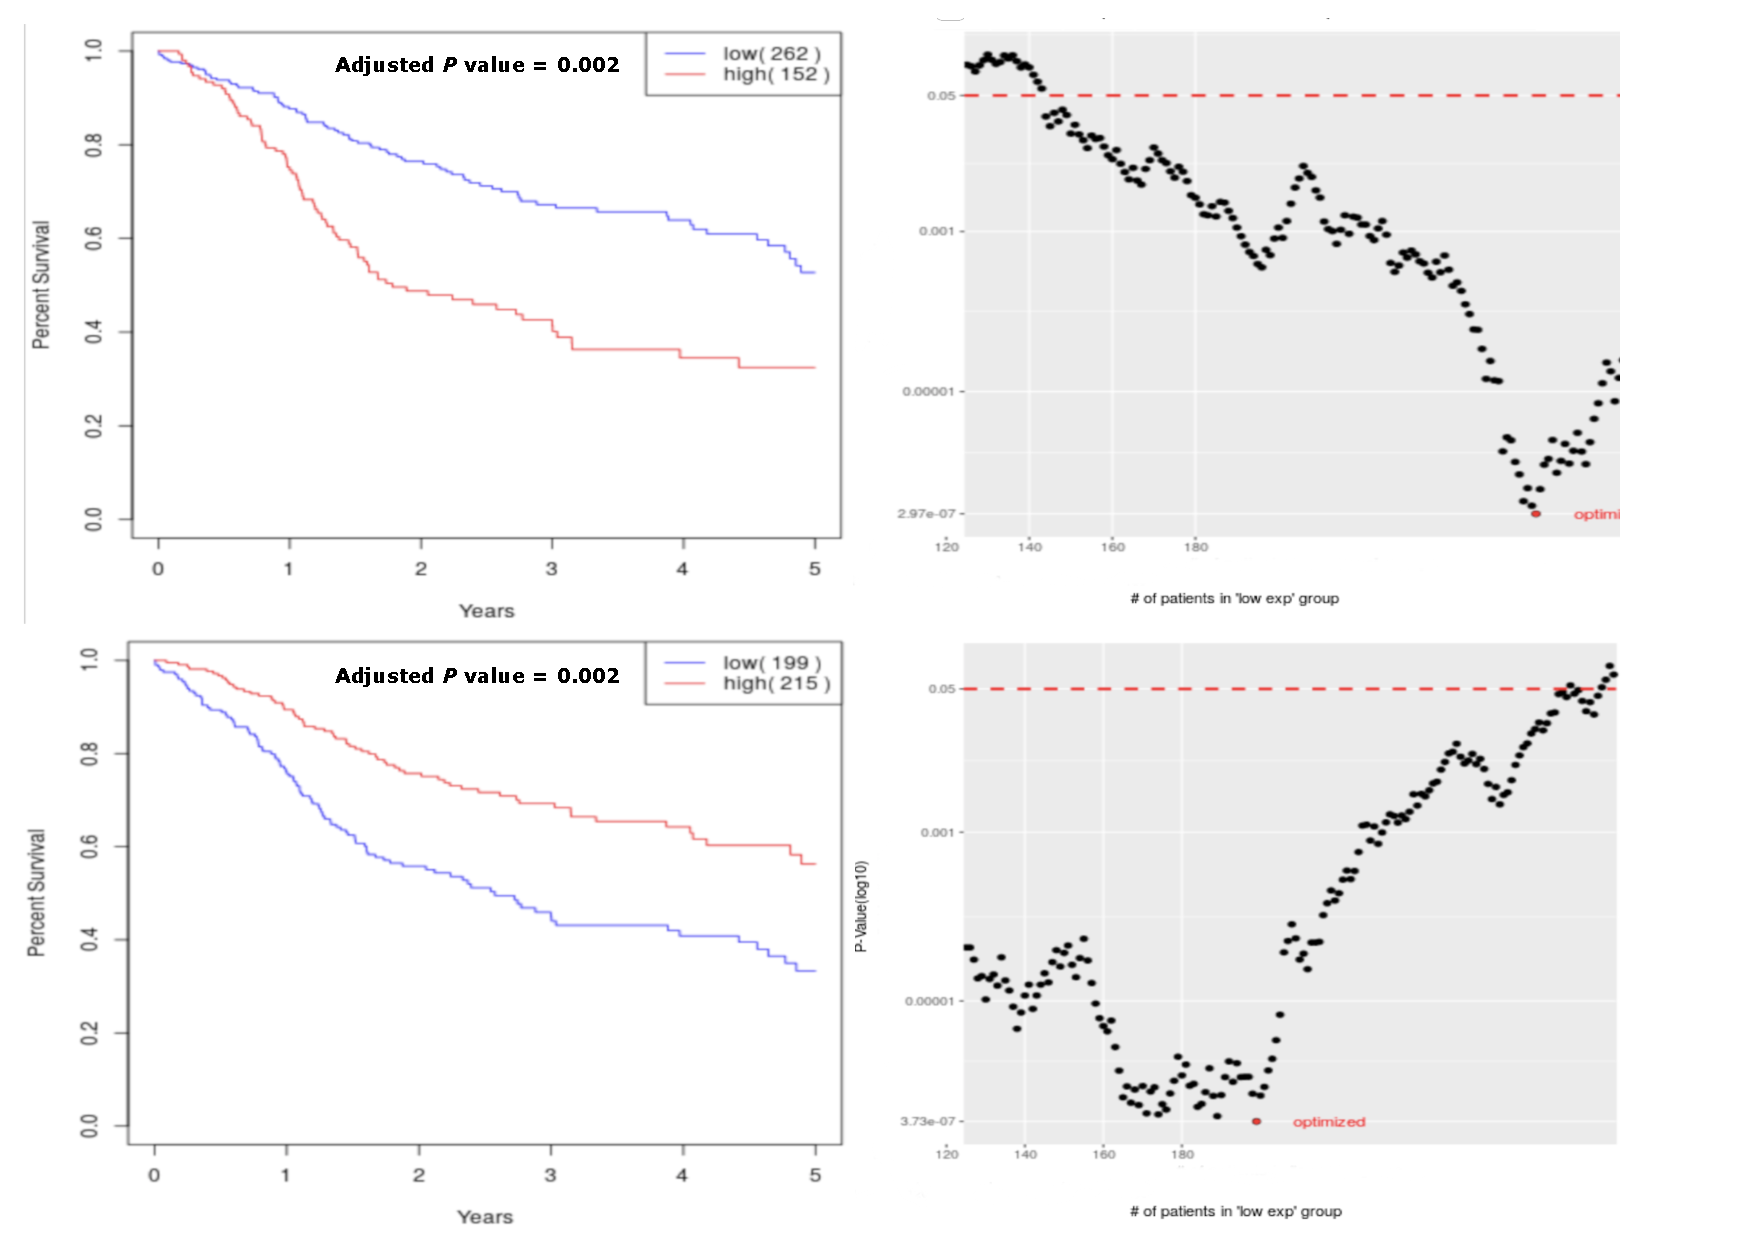
\includegraphics[width=15cm]{Figure_4_CAMK2N1_IL19.pdf}
%\draw[annotation left = {Aries at 0.3}]

%\end{annotationimage}
\end{picture}%

\bcaption{Kaplan-Meier survival analyses, by cutoff finding.}
{The Kaplan-Meier curves of (a) CAMK2N1, (c) CALML5, and (e) FCGBP under optimal \textit{P} value. 
%((b) the cutoffs derived from it's cumulative \textit{P} value plot).
%(c) Kaplan-Meier plot of IL19 under optimal \textit{P} value;
%((d) the cutoffs derived from it's cumulative \textit{P} value plot).
%(e) Kaplan-Meier plot of FCGBP under optimal \textit{P} value.\\
The cutoffs, in the cumulative \textit{P} value plots of (b) CAMK2N1, (d) CALML5, and (f) FCGBP, respectively,
shows that over 50\% of those unadjusted \textit{P} values are below 0.001 derived by sliding-window cutoff finding procedure.\\
* \textit{P}: Adjusted \textit{P} value by \acrfull{fdr}
}
\label{fig:figure4}
\end{figure}



%as Rplot_pvaluePlot_NDFIP1.pdf
%Moreover, in the special case, one of our 20 preliminary candidates, gene "NDFIP1", 



% supplementary figure
\begin{figure}[ht]
    \centering
    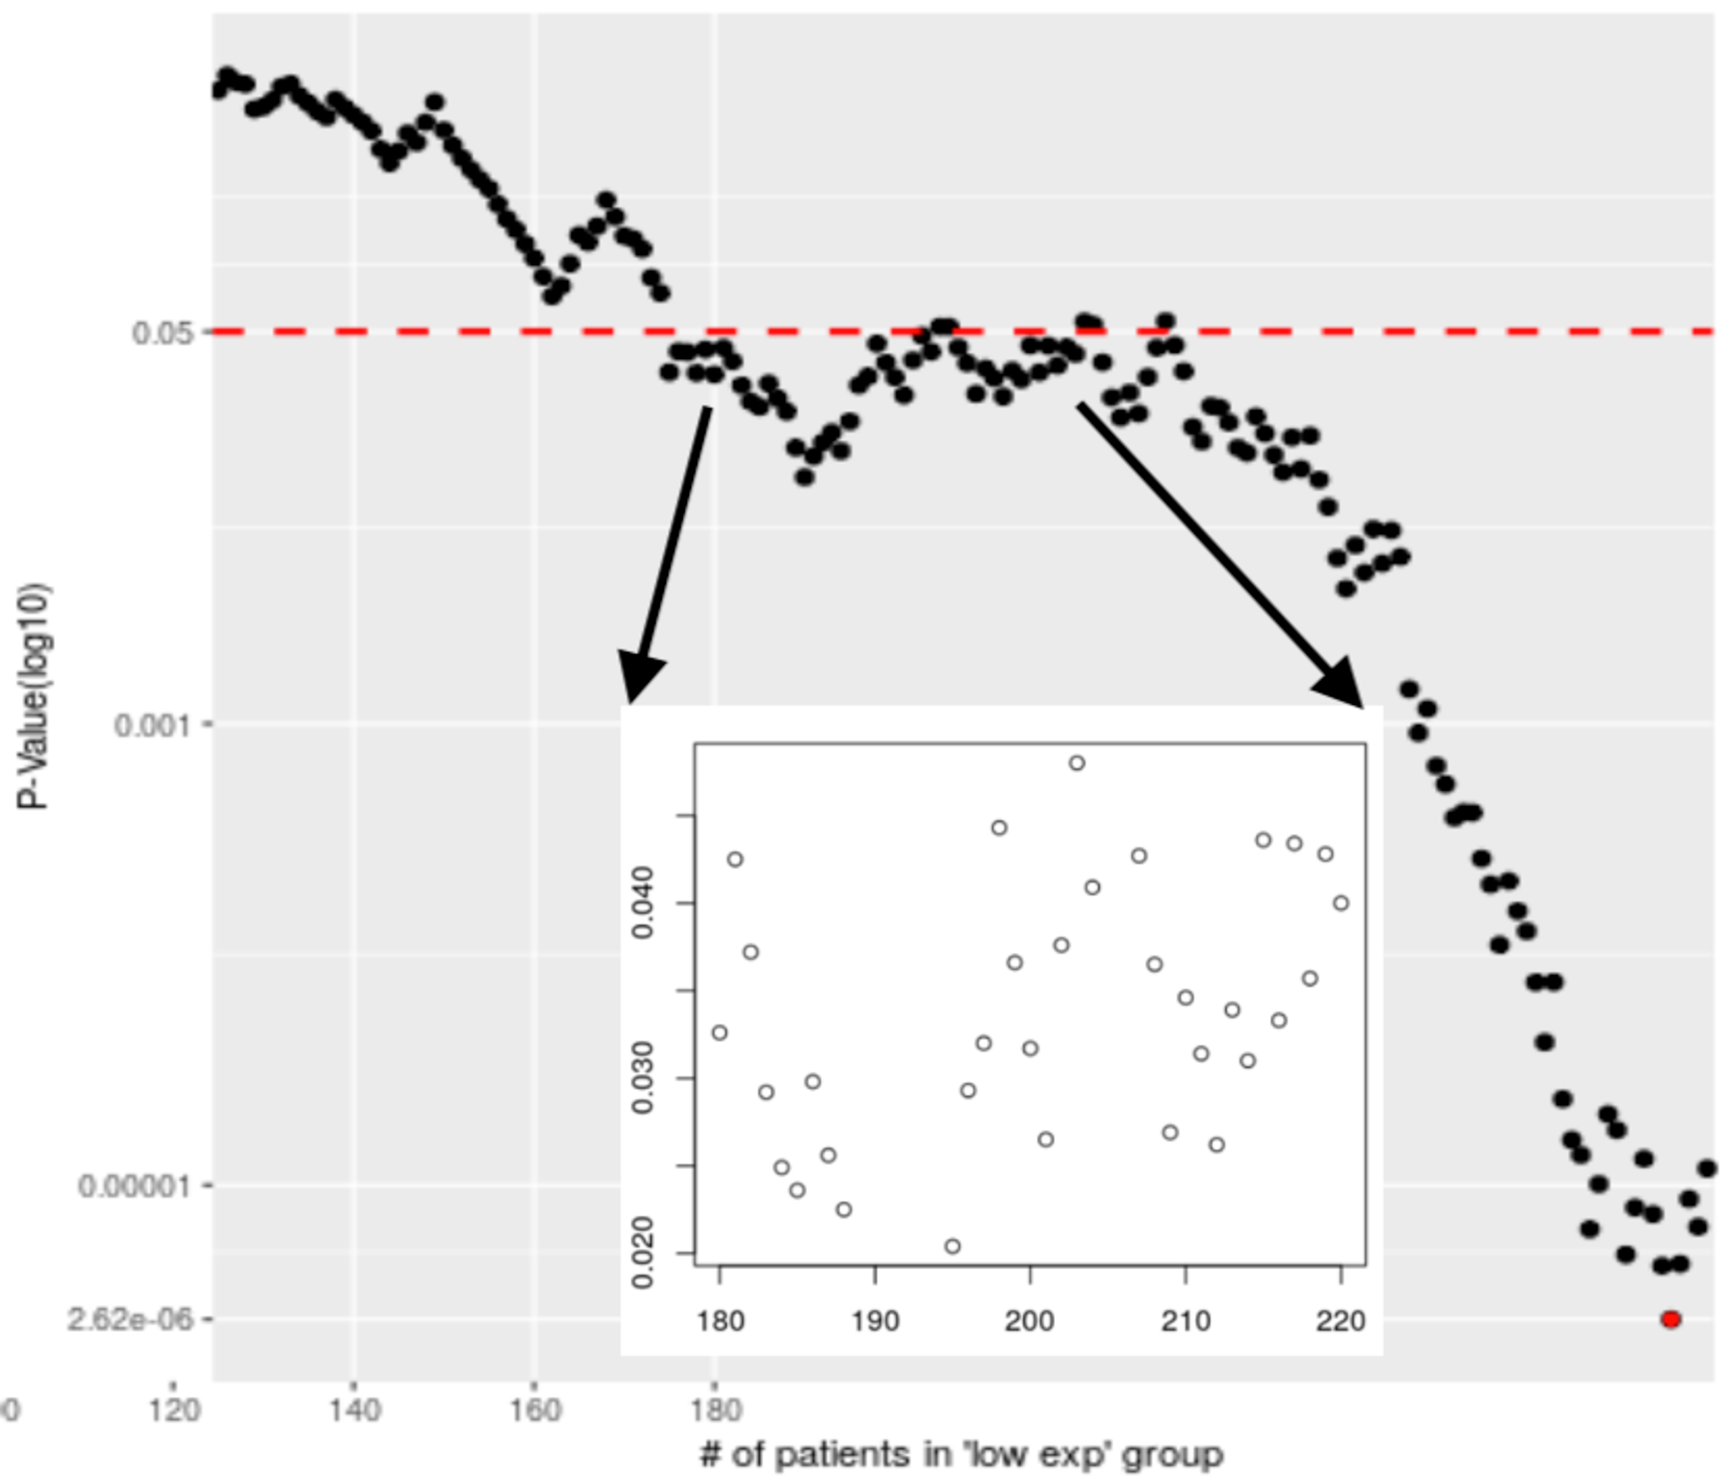
\includegraphics[width=10cm]{Rplot_pvaluePlot_NDFIP1.pdf}
    \caption{Under cutoff-finding procedure of Kaplan-Meier analysis, the \textit{P}-value plot of gene "NDFIP1" shows: 1) 70\% of \textit{P} values is $<0.05$; 2) the median-cut zone (zoom-in and revealed in inset box) has a "W"-like distribution; 3) sliding-window cutoff selection could find it's optimized \textit{P} values (far less than 0.001) while a median cut might yield \textit{P} value $>=0.05$.\\
    (x-axis: grouping by person number; y-axis: \textit{P} value in log10 transformed)}
    \label{fig:pvaluePlot_NDFIP1}
\end{figure}

%There is so many thing we could find during the data mining from so many 20500 protein-coding genes.
We performed the FDR correction applied on the Kaplan-Meier \textit{P} values of cutoff finding procedure, then Bonferroni adjustment of those \textit{P} values for candidate selection.
%\begin{MyColorPar}{red}
%\end{MyColorPar}
% and FDR (done; ok)
We modified Figure 5 (with three candidates) and the last paragraph of "Cutoff Finder Core Engine" in the Materials and Methods section.
%Figure 1, Table 1, 2 correction: Kaplan-Meier FDR correction
%***The caption of Figure 1 and Table 1 has description about 1) FDR correction of Kaplan-Meier \textit{P} values during Cutoff finding; and 2) Bonferroni correction of Kaplan-Meier \textit{P} values after Cox modeling for candidate selection.
The paragraphs marked in \textcolor{red}{Red} from page 16 (line 502 to line 505) are the part of the manuscript that has been revised. Also, it is shown here in the following paragraph.
\\[0.3cm]


\begin{MyIndent}
\begin{MyColorPar}{red}
% TCGA_HNSCC_marginSFP.R [line 111] cutoffReturn <- cutofFinder_func_HNSCC.R
% retrieving optimized (minimal) p value of each Kaplan-Meier plot 
% **A summary table of P-value, Z-score standardization from all HNSCC_survival*.Rda 
% 不必每次重 run (saved at HNSCC_OS_marginS_pvalueKM_candidate_cox.Rda)
% variable name: candidate_sample (with gene symbol and KM p value), candidate_cox, n_percent_Bonferroni
%=> FDR() or p.adjust() The FDR function uses the Benjamini & Hochberg (\cite{Benjamini1995a}) ("BH", alias "fdr") correction by default.
% analysis_export.R [line 197] has FDR < 0.05 for filtering (done)
% [line 196] OS_pvalueS$p_value_adj_FDR <- p.adjust(OS_pvalue$p_OS, method='fdr')

% (stored at HNSCC_survivalAnalysis_marginS_[gene].Rda; file20500_list.txt)
"
The \acrfull{fdr} ($< 0.05$) correction\cite{Benjamini1995a} shows which genes should be retained for subsequent univariate and multivariate analysis.
% of Cox modeling
It ensures the control of type I error of multiple test \textit{P} values during our cutoff finding procedure.
Then Bonferroni adjustment of that \textit{P} values has been used for candidate selection.
"
\end{MyColorPar} % red
\end{MyIndent}

\end{MyColorPar}
%***=> Bonferroni correction should be used in final decision.


%\begin{MyColorPar}{red}

%\end{MyColorPar}



%
\clearpage
\subsection*{2-2}
%(OK)
I recommend the authors weaken their statement of the workflow but focus on the identified biomarkers in neck squamous cell carcinoma and use as much as possible evidence to support or validate them. % new Title, abstract, change tone


%
\begin{MyColorPar}{blue}
Answer
%(OK)
We appreciate the reviewer for the critical comment.
We changed title, "Transcriptomic Analysis for Prognostic Value in Head and Neck Squamous Cell Carcinoma", and abstract; we also changed the tone in our manuscript to focus on the identified biomarkers in the head and neck squamous cell carcinoma.
There is more evidence to validate them (please see Answer 2-3).

%
\end{MyColorPar}



\subsection*{2-3}
% ( ) not yet for discussion 1) sample size/effect size; 2) ***NDFIP1
% [2021/06/17]
% PPV positive prediction value => prevalence-sensitive (COVID-19 盛行率的觀念一致) ROC from sensitivity and specificity (less biomarkers but more P value < 1e-5?)

% strategy should changing; run GCP Rstudio 框列更多的 candidates for GEO (GSE65858) during candidate selection
In the independent test, half genes have p-values less than 0.05, and most of them have p-values $> 0.01$. % table 1 => this is Bonferroni 的結果
Purely based on the number of genes and their p-values, the validation rate is relatively low, and the usability of the biomarkers is questionable. % the validation rate 
The p-values are affected by the sample size, which should be described in the main text. % writing (ok) [2021/06/26]; also affecting the over-fitting during a model training
As I mentioned above, the authors should look for more data to verify these biomarkers. % GEO GSE65858(ok) 
%or even GSE117973? GPL10558	Illumina HumanHT-12 V4.0 expression beadchip; https://www.ncbi.nlm.nih.gov/geo/geo2r/?acc=GSE117973
% Progression-free survival (PFS) is "the length of time during and after the treatment of a disease, such as cancer, that a patient lives with the disease but it does not get worse".[1] In oncology, PFS usually refers to situations in which a tumor is present, as demonstrated by laboratory testing, radiologic testing, or clinically. Similarly, "disease-free survival" is when patients have received treatment and are left with no detectable disease.
% disease-specific survival rate: The percentage of people in a study group who have not died from a specific disease in a defined period of time. The time period usually begins at the time of diagnosis of the disease and ends at the time of death from the disease. 
%Patients who died from causes other than the disease being studied are not counted in this measurement.



%
\begin{MyColorPar}{blue}
Answer\\


% the validation rate
% more GSE datasets; pick-up more candidate (run GCP) in hands 而且要偷看答案
% x using  receiver operating characteristic (ROC) analysis and more GEO datasets
We appreciate the reviewer for the critical comments and thanks for the guidance of our work in cancer research.
% workflow 更加嚴格以增加 validation rate
%Validation rate:\\
%x重新挑選 candidate (FDR100) (GSE2837 and GSE65858)
% => answer is: consensus top3 genes
% (ok) Table 1/2 caption, Fig KP plot: FDR P value (要改為真的FDR) [line 196]
% [2021/06/11]決議;
We have introduced an independent HNSCC cohort (GSE65858, with RNA-Seq expression data) for helping in candidate selection.
We have also performed Kaplan-Meier and Cox survival analyses, under the cutoff of each gene expression at their median value.
%We further
%validate them by using a independent HNSCC cohort (GSE65858, with RNA-Seq expression data)

% problem of it (少 n=30, and RFS only: validation rate 14/100 而且 10% cutoff)
%x Prognoscan (GSE2837) (n=30 less)  RFS only:  10\% cutoff to yield a \textit{P}-value < 0.05.\\
%找出  3 candidates
During our exploration phase with TCGA cohort, the 20 genes, listed
%six overexpressed genes (symbol as CAMK2N1, PGK1, SURF4, USP10, NDFIP1, FOXA2) are bad guy;
%four overexpressed genes (symbol as IL19, FCGBP, IQCN - former symbol as KIAA1683, and NPB) are good guy.
%}
in Figure \ref{fig:hazards3}, have FDR-adjusted \textit{P} values ($<0.001$) in Kaplan-Meier estimate, and survival impact on HR ($> 1.8$ or $< 0.6$) in Cox's model.
%
% [2021/06/13-17]
%CAMK2N1, IL19, and FCGBP is validated by
%candidate_fdr100
%PvalueTex consensus with GSE2837 to yield 3 candidates
In the study of GSE65858 cohort, CAMK2N1, CALML5, and FCGBP, keep ahead of the curve by their FDR-corrected \textit{P} value ($< 0.05$), and Cox'HR ($>1.8$ or $<0.6$) (please see Table \ref{tab:table_top3_GSE65858} listed below,
% (ok) (FDR KM \textit{P} value) <= # only MSMB KM FDR-adjusted P value = 0.002 
% Consensus 3 genes in Kaplan-Meier survival and Cox's model (dataset: GSE65858)
%Gene.Symbol KM.Pvalue   FDR.KMpvalue    uni_HR  FDR.Pvalue(in TCGA)
%CAMK2N1 0.00687 0.03782500  1.814   1.628308e-05
%FCGBP   0.01020 0.03886709  0.573   4.827833e-05
%IL19    0.03390   0.04738901    0.630   6.543871e-06
%IL19    0.00269  0.03068073 0.630  6.543871e-06
%candidate_fdr100
and also see Figure \ref{fig:hazards534}).
However, the "top rank" of the other 17 genes is replaced by genes such as DUSP6, MSMB, and RBM11 (please see Figure \ref{fig:hazards534}).
There is consensus between the TCGA and GSE65858 cohorts that CAMK2N1, CALML5, and FCGBP are significant candidates for the biomarker.
%In the consensus of TCGA and GSE65858 cohorts, 

%Rplot_GSE65858_CoxHR_CAMK2N1_top3FDRKM.pdf % FDR KM p value of hazards534
% by Validation_GSE65858_survival.R
% Rplot_GSE65858_CoxHR_CAMK2N1_validated.pdf
\begin{figure}
    \centering
    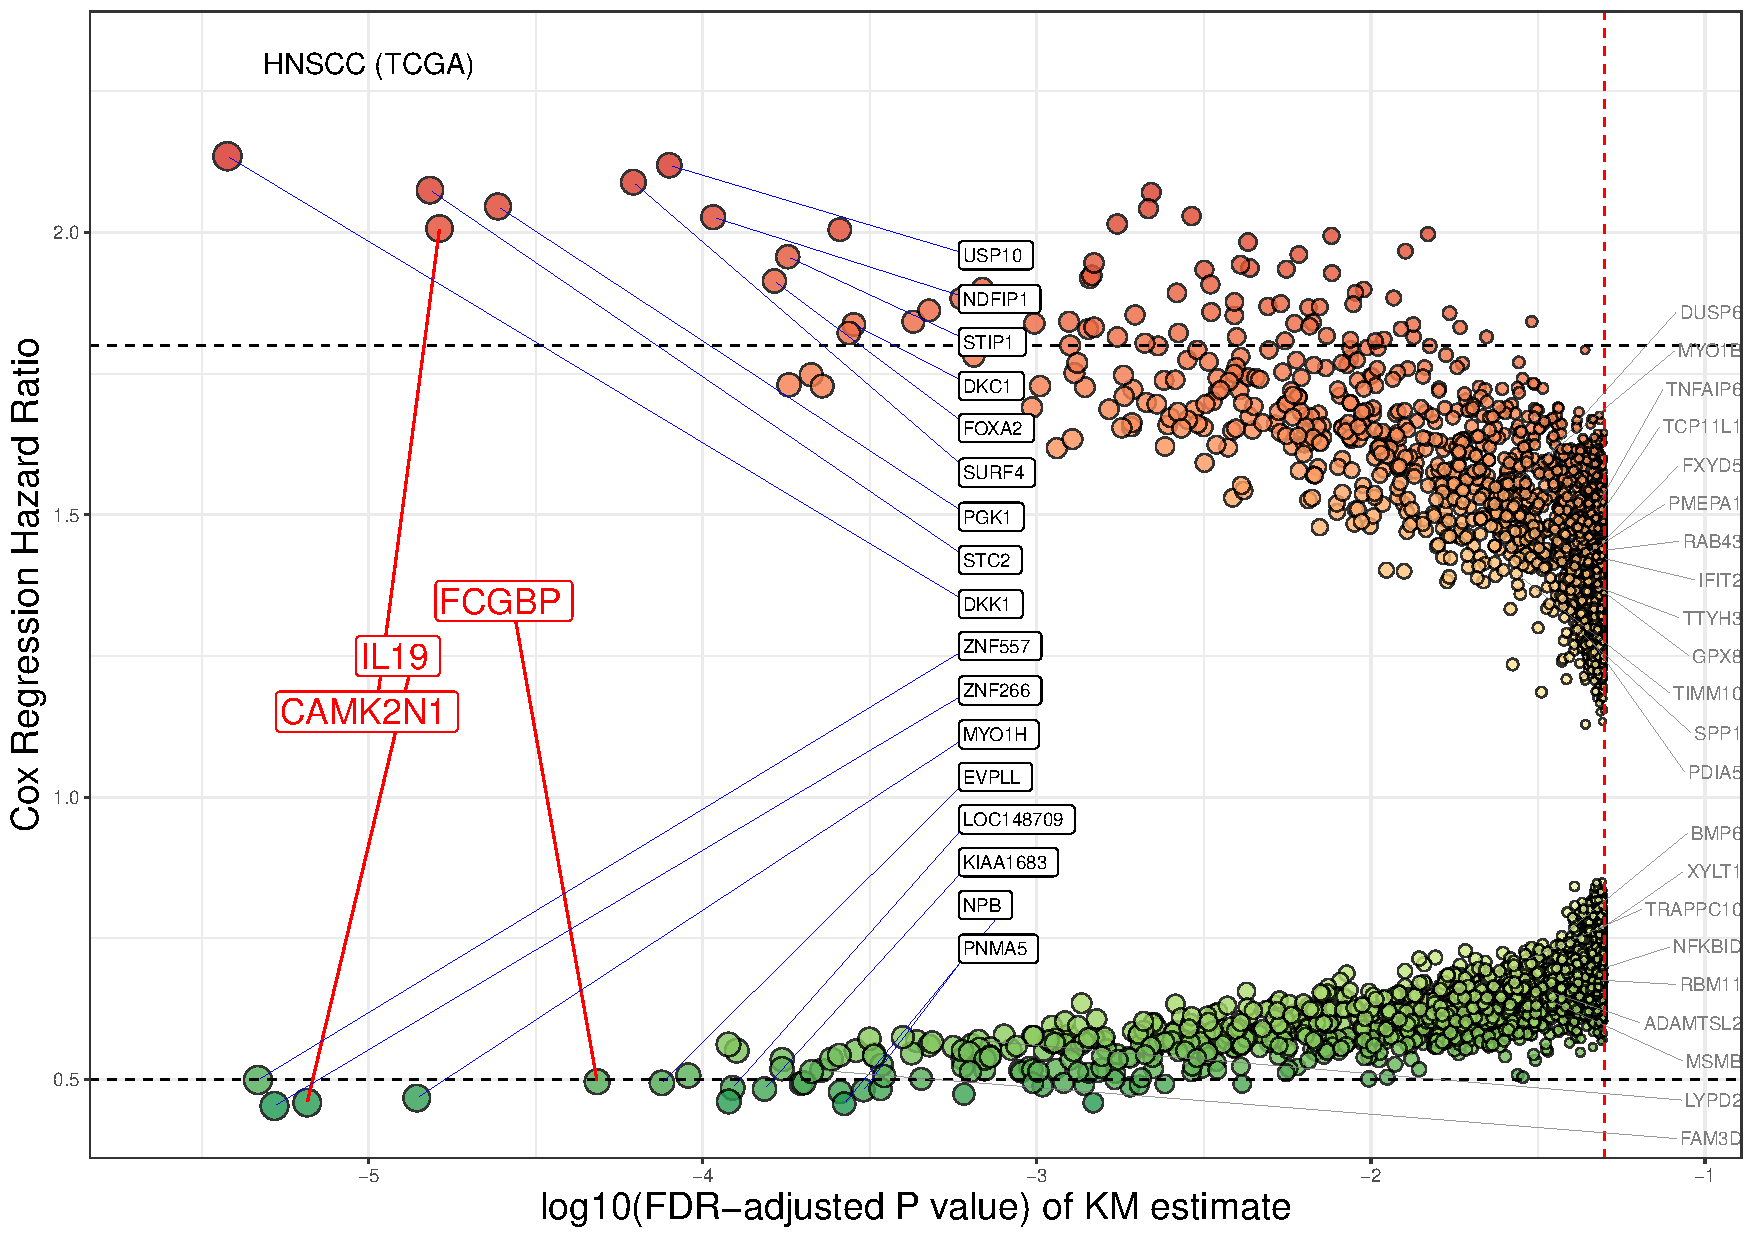
\includegraphics[width=13cm]{Rplot_TCGA_HNSCC_CoxHR_CAMK2N1_top3FDRKM.pdf}
    \bcaption{Volcano plot of genes under survival analyses of TCGA HNSCC.}{
%X axis: unadjusted \textit{P} value of Kaplan-Meier survival (-log10 transformed).
%Y axis: multivariate hazard ratio from Cox proportional regression model.
%Dotted line: significant Bonferroni corrected \textit{P} value. 
%\textcolor{red}{Red dots} mark 10 genes (unvalidated), which impact on poor prognosis ($HR>=1.5$). \textcolor{green}{Green dots} mark 10 genes (unvalidated), which affect on better survival ($HR<=0.5$).
    This cohort has been applied for exploration of the candidate biomarkers.
    Total 9416 genes has %\acrshort{fdr}-
    unadjusted \textit{P} value less than 0.05.
    \textcolor{red}{CAMK2N1}, \textcolor{red}{CALML5}, \textcolor{red}{FCGBP} and the 17 genes (marked in \textcolor{black}{black square}) have hazard ratio (HR) $> 1.8$ or $< 0.6$.
    The 22 genes, listed on the side, have hazard ratio between 0.6 and 1.5.\\
    Remarks:\\
    \textcolor{red}{Red spots}: $HR > 1.0$;
    \textcolor{green}{Green spots}: $HR < 1.0$;\\
    X-axis: Kaplan-Meier survival estimates, with \acrshort{fdr}-adjusted \textit{P} value (log10 transformed);\\
    Y-axis: HR of Cox proportional hazard regression model\\
    }
    \label{fig:hazards3}
\end{figure}


% Please add the following required packages to your document preamble:
% \usepackage{graphicx}
% Please add the following required packages to your document preamble:
\begin{table}[ht]
\centering
\caption{The consensus between the TCGA and GSE65858 cohorts in Kaplan-Meier survival and Cox's model}
\label{tab:table_top3_GSE65858}
\resizebox{\linewidth}{!}{%
\begin{tabular}{llllclc}
\hline
%\multirow{2}{*}{}
Gene Symbol &
  \multicolumn{2}{c}{KM \textit{P} value} &
  \multicolumn{2}{c}{FDR-adjusted \textit{P} value} &
  \multicolumn{2}{c}{Cox’s univariate HR} \\
%  \hline
 &
  \multicolumn{1}{c}{TCGA} &
  \multicolumn{1}{c}{GSE65858} &
  \multicolumn{1}{c}{TCGA} &
  \multicolumn{1}{c}{GSE65858} &
  \multicolumn{1}{c}{TCGA} &
  \multicolumn{1}{c}{GSE65858} \\
  \hline
  \hline
CAMK2N1 & \num{2.97e-7} & \num{6.87e-3} & \num{1.63e-5} & 0.038 & 2.101 & 1.814 \\
CALML5    & \num{5.87e-6}  & \num{4.75e-3}          & \num{1.97e-4}          & 0.035 & 0.493   & 0.541  \\
IL19    & \num{3.73e-7} & \num{2.69e-3} & \num{6.54e-6} & 0.031 & 0.472 & 0.630  \\
FCGBP   & \num{1.21e-6} & 0.01          & \num{4.83e-5} & 0.039 & 0.484 & 0.573\\
\hline
%  \multicolumn{7}{l}{(IL19 has two probes in RNA-Seq experiment of GSE65858)}\\
  \multicolumn{7}{l}{(FDR: \acrlong{fdr}; HR: hazard ratio)}\\
\hline
\end{tabular}%
} % end of \resizebox
\end{table}

%Rplot_GSE65858_CoxHR_CAMK2N1_top3FDRKM.pdf % FDR KM p value of hazards534
% by Validation_GSE65858_survival.R
% Rplot_GSE65858_CoxHR_CAMK2N1_validated.pdf

\begin{figure}
    \centering
    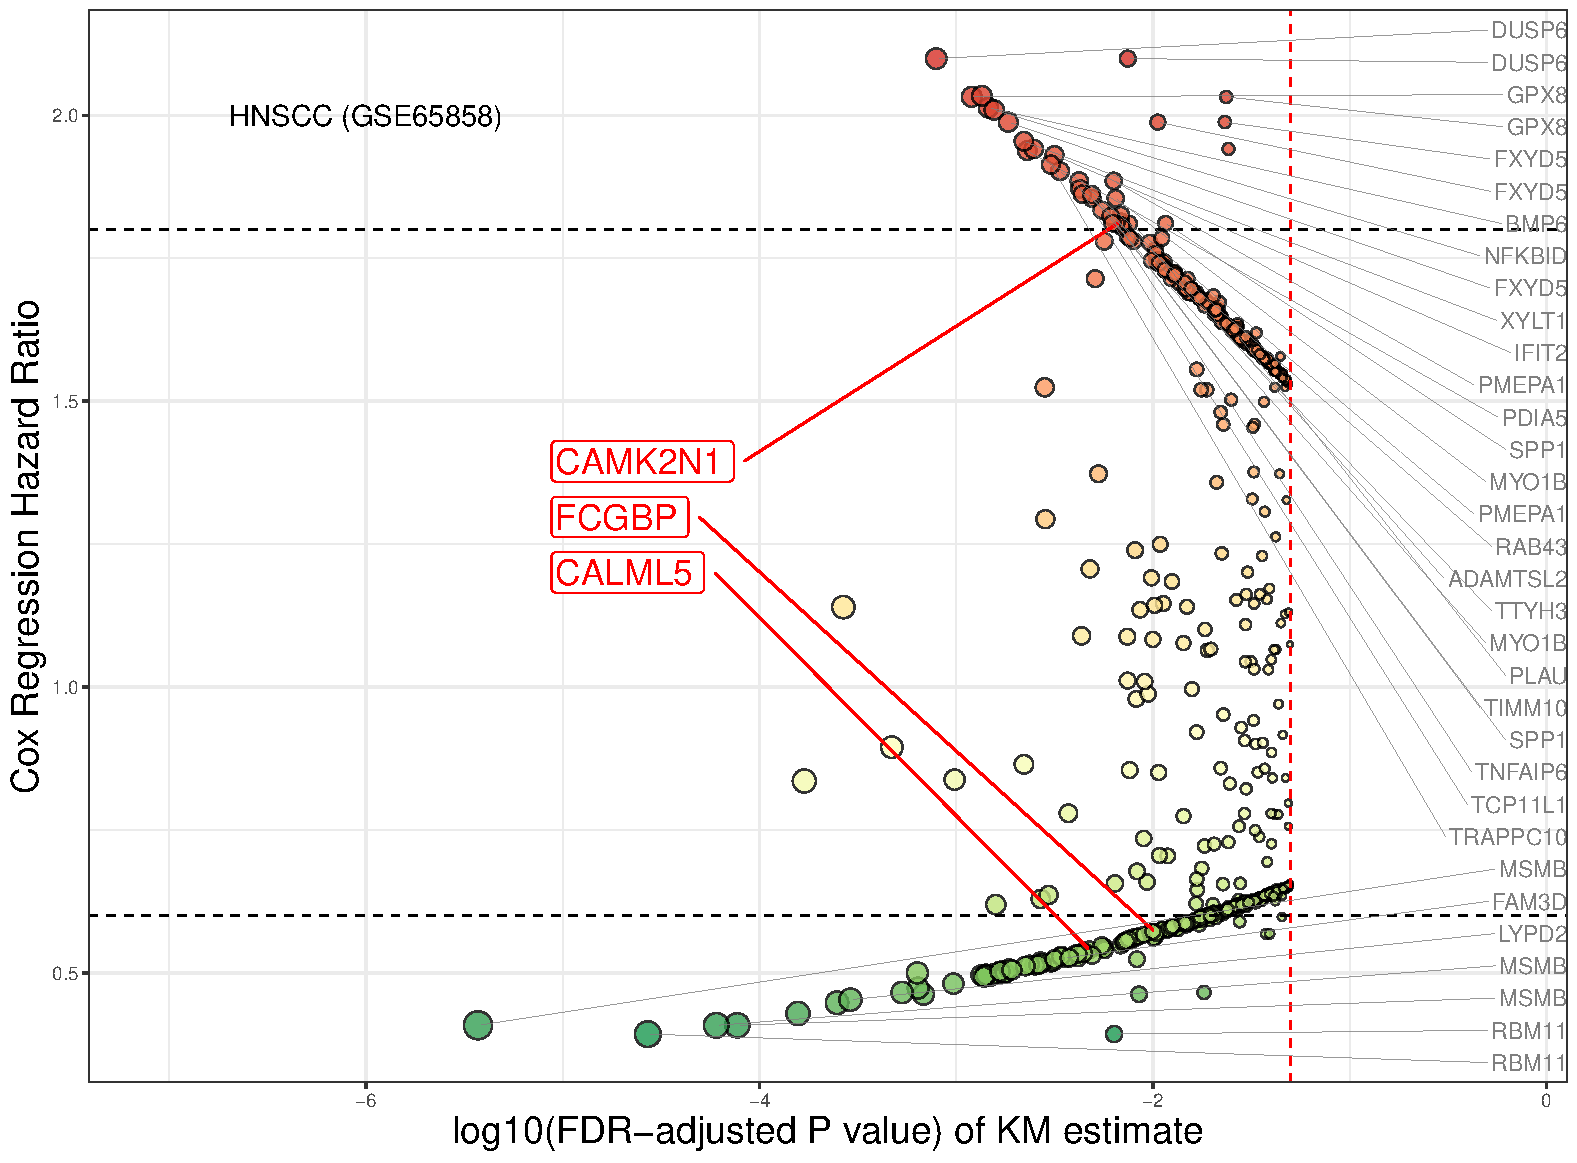
\includegraphics[width=13cm]{Rplot_GSE65858_CoxHR_CAMK2N1_top3FDRKM.pdf}
    \bcaption{Volcano plot of genes under survival analyses of GSE65858 cohort}{
    % GSE117973 using the same platform GPL10558
    This HNSCC cohort has been applied for filtering of our candidate genes: \textcolor{red}{CAMK2N1}, \textcolor{red}{CALML5}, and \textcolor{red}{FCGBP}.
    Total 534 genes has \acrshort{fdr}-adjusted \textit{P} value less than 0.05
    (\textcolor{red}{Red spots}: hazard ratio is greater than 1.0);
    (\textcolor{green}{Green spots}: hazard ratio is under than 1.0).\\
    The 22 genes, listed on the side, have hazard ratio $> 1.8$ or $< 0.6$.\\
    (X-axis: Kaplan-Meier survival estimates, with \acrshort{fdr}-adjusted \textit{P} value with log10 transformed);
    (Y-axis: the hazard ratio (HR) under Cox proportional hazard regression model)
    }
    \label{fig:hazards534}
\end{figure}



% SurvExpress http://bioinformatica.mty.itesm.mx:8080/Biomatec/SurvivaX.jsp
%x Saintigny Mao Survival Oral cancer GSE26549 (n=86) with features of OSCC outcome (no time), Gender, Race, Alcohol, and Smoking.
%Petel Head and Neck Squamous Cell Carcinoma E-MTAB-1328 (n=89) RFS(metastasis) with time
% https://www.ebi.ac.uk/arrayexpress/experiments/E-MTAB-1328/
%Chung Parker Head and Neck GSE10300 (n=44), RFS with time

%TCIA CPTAC (not HPA 抗體很少)
%This collection contains subjects from the National Cancer Institute’s Clinical Proteomic Tumor Analysis Consortium Head-and-Neck cancer (CPTAC-HNSCC) cohort.
%https://wiki.cancerimagingarchive.net/display/Public/CPTAC-HNSCC
%As digital tissue microarray? 


%GSE117973
%***  (GSE117973) Patients of the Heidelberg Center for Personalized Oncology-Head and Neck Cancer (HIPO-HNC) cohort (n = 87, GSE117973) were treated between 2012 and 2016 at the University Hospital Heidelberg, Germany.
%PFS and DSS event and months.



We modified the paragraphs in the "Materials and Methods" section, and "Results" section for the analysis of GSE65858.
We also described "the \textit{P} values are affected by the sample size" in the "Discussions" section.
% ok
The paragraphs in "Materials and Methods" marked in \textcolor{red}{Red} on page 18 (line 560 to line 572),
% results ok
the paragraphs in "Results" marked in \textcolor{red}{Red} from page 5 (line 148) to page 6 (line 172) , and
% ok
the paragraphs in "Discussions" marked in \textcolor{red}{Red} from page 10 (line 236) to page 11 (line 280)
are the part of the manuscript that has been revised. 
Also, it is shown here in the following paragraph.
\\[0.3cm]

\begin{MyIndent}
\begin{MyColorPar}{red}

%%%
% (OK)*the authors should look for more data to verify these biomarkers.
%For validation by GEO datasets:

\textcolor{blue}{In the section of Materials and Methods}\\
%RefSeq Release 38 (November 7, 2009)  GSE65858
%[Dataset]
"
The Gene Expression Omnibus (GEO) database, founded by \acrfull{ncbi}, is a public repository supporting MIAME-compliant data submissions of microarray and sequence-based experiments.
R package of \\GEOquery\cite{Sean2007} was used to
download RNA-Seq dataset (in SOFT or MINiML format) of a HNSCC cohort, GSE65858, from the GEO database (available at https://www.ncbi.nlm.nih.gov/geo/\\geo2r/?\\acc=GSE65858). 
GSE65858\cite{Wichmann2015} has OS event, RFS event, and survival time.
There are 270 HNSCC participants involved in this cohort.
%The number of genes (or probes of RNA-Seq in platform GPL10558, Illumina HumanHT-12 V4.0 expression beadchip) is 30,330.
%n=270 n= 273 = ?? + 168(alive) + 88(dead) = 256
The expression data was generated using the platform GPL10558 (Illumina HumanHT-12 v4.0 Expression BeadChip), which targets on more than 30,330 annotated genes (47,000 probes, derived from the \acrshort{ncbi} Reference Sequence, release 38 on Nov 7, 2009). % (RefSeq) 
GSE65858 is a dataset for candidate selection in our workflow.
We have also performed Kaplan-Meier and Cox survival analyses under the cutoff of each gene expression at their median value.\\
"

\textcolor{blue}{In the section of Results}\\
"
TCGA HNSCC cohort was applied for exploration of the biomarker candidate.
A total of 9416 Kaplan-Meier plots (under sliding-window cutoff selection) with associated Cox's univariate and multivariate tables were generated by Cox modeling (see Figure \ref{fig:figure1}) and justified by the ranking of hazard ratios.
%The ten genes, named DKK1, CAMK2N1, STC2, PGK1, SURF4, USP10, NDFIP1, FOXA2, 
The 967 out of 9416 genes were kept by criteria of Kaplan-Meier \textit{P} value ($< 0.05$) and \acrfull{hr} derived from Cox's model (please see Figure 2(a), (b), initial trial).
In the next step, a Bonferroni P-value correction was used to yield 20 genes, under the stringent criteria (see Figure 2(c), (d)).
%em dash ---
These CAMK2N1, CALML5, FCGBP and the other 17 genes (DKK1, STC2, PGK1, SURF4, USP10, NDFIP1, FOXA2, STIP1, DKC1, ZNF557, ZNF266, MYO1H, EVPLL, PNMA5, IQCN, NPB, and CALML5) have significant FDR-adjusted \textit{P} values ($< 0.0003$) in Kaplan-Meier estimate, and greater hazard ratio (HR) ($> 1.8$ or $< 0.6$) in Cox's model (please see Figure \ref{fig:hazards3}; $log_{10}(0.0003) = -3.5$).
%These genes have also passed a stringent criteria (Bonferroni \textit{P} value correction less than 0.05).
The plot reveals that the top 20 genes (Bonferroni-adjusted \textit{P} $< 0.05$) are located on the peaks. At the same time, Cox's HR separates them on the two-side with significant prognostic impact.
%During our exploration phase with TCGA cohort, the 20 genes, listed
%six overexpressed genes (symbol as CAMK2N1, PGK1, SURF4, USP10, NDFIP1, FOXA2) are bad guy;
%four overexpressed genes (symbol as IL19, FCGBP, IQCN - former symbol as KIAA1683, and NPB) are good guy.
%}
%in Figure \ref{fig:hazards3}, have FDR-adjusted \textit{P} values ($<0.001$) in Kaplan-Meier estimate, and survival impact on HR ($> 1.8$ or $< 0.6$) in Cox's model.

% [2021/06/13-17] GSE65858
%CAMK2N1, IL19, and FCGBP is validated by
%candidate_fdr100
%PvalueTex consensus with GSE2837 to yield 3 candidates
In the study of GSE65858 cohort with median cutoffs, CAMK2N1, CALML5, and FCGBP (3 of the 20 genes), keep ahead of the curve by their FDR-corrected \textit{P} value ($< 0.05$), and Cox's HR ($>1.8$ or $<0.6$) (please see Table \ref{tab:table_top3_GSE65858} listed below,
% (ok) (FDR KM \textit{P} value) <= # only MSMB KM FDR-adjusted P value = 0.002
% Consensus 3 genes in Kaplan-Meier survival and Cox's model (dataset: GSE65858)
%Gene.Symbol KM.Pvalue   FDR.KMpvalue    uni_HR  FDR.Pvalue(in TCGA)
%CAMK2N1 0.00687 0.03782500  1.814   1.628308e-05
%FCGBP   0.01020 0.03886709  0.573   4.827833e-05
%IL19    0.03390   0.04738901    0.630   6.543871e-06
%IL19    0.00269  0.03068073 0.630  6.543871e-06
%candidate_fdr100
and also see Figure \ref{fig:hazards534}).
However, the significance of the other 17 genes are replaced by genes such as DUSP6, MSMB, and RBM11 (please see Figure \ref{fig:hazards534}).
%This GSE65858 cohort has been applied for selection to generate our candidate genes: \textcolor{red}{CAMK2N1}, \textcolor{red}{IL19} (two probes), and , \textcolor{red}{FCGBP}.
Conversely, there are 22 genes, which have greater hazard ratio ($> 1.8$ or $<0.6$) in GSE65858 cohort (Figure \ref{fig:hazards534}), drop their hazard ratio between 0.6 and 1.5 in the study of TCGA HNSCC (Figure \ref{fig:hazards3}).
Thus, there is a consensus between the TCGA and GSE65858 cohorts that CAMK2N1, CALML5, and FCGBP are significant candidates for the HNSCC biomarker.
%Finally, these 3 candidates were also confirmed by a HNSCC study using the GSE2837 dataset. Please see the Kaplan-Meier plots in Supplementary Figure S2.%\ref{fig:fig_GSE2837}.
"\\[0.3cm]
%The consensus between the TCGA and GSE65858 cohorts in Kaplan-Meier survival and Cox's model
%by GEO GSE2837 HNSCC dataset (PrognoScan)
%After the discovery by our workflow, we validated the those 20 genes in the other independent \acrshort{hnscc} cohort (GSE2837).
%The survival significance (Kaplan-Meier \textit{P} value) is in the following probes among 10 genes:\\
%1) poor prognosis: CAMK2N1 (0.048214), PGK1 (0.009978), SURF4 (0.023127), USP10 (0.017768), NDFIP1 (0.022758), FOXA2 (0.001587);\\ % FOXA2 (0.038125)
%2) better prognosis: IL19 (0.049731), FCGBP (0.005658), KIAA1683 (IQCN, 0.005886), NPB (0.014177);\\
%17 out of 20 candidates


\textcolor{blue}{In the Discussions section}\\
% %\subsection{The Purpose of a Sliding-window Cutoff Selection}
%[more in the discussion section]
  % (ok)
"
%%% Statistical significance (\textit{P} value) is affected by both sample size, error, effect size (substantive significance)\cite{Sullivan2012}\cite{Thiese2016}, and cutoff.
%\subsection{The Purpose of a Sliding-window Cutoff Selection}
% risk of *** Answer 2-3 併入此
%Second, t
Trying to find an optimal cutpoint of that \acrshort{rna} expression data to maximize candidate mining coverage, this strategy could identify more but sometimes weak "biomarkers".
%We have checked this issue in detail (in the Discussions section).
%Thus, the false positives and adjustment of multiple comparisons should be corrected by \acrfull{fdr}.
Thus, we should try our best to handle the effect size from Cox's modeling.
And validation of those candidates is required by using other independent dataset.
% in larger patient populations.% in larger patient
%warrant.

Statistical significance (\textit{P} value) is affected by both sample size, error, effect size (substantive significance)\cite{Sullivan2012}\cite{Thiese2016}, and cutoff. 
The effect size is the magnitude of the difference (e.g., \acrlong{hr}) among comparing groups.
%A \textit{P} value is a tool to help interpret findings from biomedical research.
%In reporting and interpreting studies, both 
%the substantive significance (effect size) and statistical significance (P value) are essential results to be reported.
%Statistical significance depends upon both sample size and effect size. 
The effect size is independent of the sample size\cite{Sullivan2012}.


%When we increase the sample size, the standard error decrease
%, or increase the difference between the sample statistic and hypothesized parameter, the p value decreases, thus making it more likely that we reject the null hypothesis.
In a study with large sample size, the difference could be noticed easily (i.e., \textit{P} value $< 0.05$) due to a decreased standard error\cite{Sullivan2012}.
However, the small effect size (non-zero) is often meaningless or substantive insignificance (e.g., hazard ratio between 0.8 and 1.2).
%With a sufficiently large sample, a statistical test will always reveal a significant difference, unless the effect size is exactly zero.
%, that is, when the effect size is exactly zero; 
%yet very small differences, even if significant, are often meaningless. 
%Thus, reporting only the significant P value for an analysis is not adequate for readers to fully understand the results.
%If the magnitude of effect is small and clinically unimportant, the p-value can be "significant" if the sample size is large.
Conversely, the effect size can be large but fail to get statistical significance if the sample size is small. 
%In this scenario, the \textit{P} value tells the effect does not exist.
The following error could also impact the \textit{P} value:
\begin{outline}
\1 A random error, defined as the variability in data, is not considered a bias but rather occurs randomly across the entire study population and can distort the measurement process (e.g., RNA-Seq experiments).
The larger sample size could reduce the random error. 
\1 A systematic error is a bias, which includes selection bias, information bias, and confounding.
It could deleteriously impact the statistical significance.
The larger sample size could not affect the systematic error.
\end{outline}
% effect size is large (whatever is true or artificial), the p value is small
While statistical significance can inform the researcher whether an effect exists, the \textit{P} value will not directly tell the effect size.
Thus, if there is no error in two study groups, and the sample size is the same (not small), the group, which has a larger effect size, will has a small \textit{P} value\cite{Thiese2016}.
%The effect size is the main finding of a quantitative study.
If a skewed cutoff that split, for example, 425 versus 75 between the two groups, it will also get statistical significance by increasing effect size artificially.
% https://stats.stackexchange.com/questions/162359/how-can-you-have-p-0-0001-with-a-sample-size-of-89-and-a-control-group-of-52
%As you can see, even with only 12 events (fustat = 1) that split 10 vs 2 between the two dummy groups you get a log-rank p-value < 0.0001.
%effect size, sample size, cutoff 影響 p value!

% [preserved] ***
%An increase in the sample size will decrease over-fitting of model[Frank Harrell].
% https://hbiostat.org/rms/

% definition of P value
%Statistical significance is the probability that the observed difference between two groups is due to chance. If the P value is larger than the alpha level chosen (e.g., 0.05), any observed difference is assumed to be explained by sampling variability.
%The most commonly used α level is 0.05, as proposed by Fischer, is the amount of type I error you are willing to accept.
%Fisher suggested 5\% (α=0.05) level could be used for concluding that fairly strong evidence exists against H0, that is 1 out of 20 times you will be wrong and by random chance there is no difference between your groups, but the data you have suggests that there is (2).

%power: Power analysis is the name given to the process for determining the sample size for a research study. The technical definition of power is that it is the probability of detecting a "true" effect when it exists. Many students think that there is a simple formula for determining sample size for every research situation.
%As the sample size gets larger, the z value increases therefore we will more likely to reject the null hypothesis; less likely to fail to reject the null hypothesis, thus the power of the test increases.

%the confidence interval of the P value (second generation P value?)

%%%%
%(ok)2-3 put in supplementary figure S1 %Rplot_pvaluePlot_NDFIP1.pdf
%from Answer 2-3 supplementary Figure S1  %圖就好 figure Rplot_pvaluePlot_NDFIP1.pdf

%2) \\
%(ok) % pvalueTex is essential; find smaller P value to predict large effect size (HR)
% The effect size is the main finding of a quantitative study.
There is a benefit for using sliding-window cutoff method (between $30\% - 70\%$ quantile) in Kaplan-Meier analysis of TCGA HNSCC cohort at the beginning.
We compared the results of cutoff at optimal \textit{P} value by sliding window or just at the median of gene expression.
It shows that the number of genes (with unadjusted \textit{P} value $< 0.05$)  is 6284 versus 3118, respectively. After FDR correction, it becomes 967 versus 209, respectively.
% HNSCC_OS_marginS_THREE_pvalue005_noCancerGene
%Result by optimal cutoff: total 9416 plots,
%6284 are raw KM P value < 0.05
%534?? genes are FDR KM P value <0.05
%967 genes which HR is greater than 1.5 or less than 0.5.
%Result by median cutoff: total 20080 genes, 
%3118 are raw KM P value < 0.05; 
%209 genes are FDR KM P value <0.05
The sliding-window cutoff method could catch more potential candidates, which have \textit{P} values far less than $0.001$, for subsequent Cox's modeling.
That is because of the properly selected cutoff improving the statistical significance.
To find a smaller \textit{P} value might predict large effect size (HR) associated biomarkers.
Then, these preliminary candidates will have an opportunity to be carefully selected by using FDR then stringent Bonferroni correction, their effect size (Cox's HR), and the other independent cohort (GSE65858) to prevent the false discovery.
% no more GSE2837
%small effect size could be double-checked by GSE65858.
%差別很大,張大網
%([2021/06/27] run code: if median cut for TCGA KM Cox by *** pvalueTex code)
%列入 workflow in materials and methods;

We explain aforementioned situation by examples.
%***NDFIP1  % 給他們一個機會
Reviewing the special case of genes, such as NDFIP1, DKC1, PNMA5, and NPB,
we noticed that NDFIP1, with a \textit{P} value of 0.05 at 50\% quantile (median) cutoff, could achieve a \textit{P} value of \num{2.62e-6} at 70\% quantile cutoff.
NDFIP1 has the FDR-adjusted \textit{P} value as \num[round-precision=3, round-mode=figures,
scientific-notation=true]{0.0001074233} (please see supplementary figure S1, a "S"- or "W"-shaped acute-bending on the \textit{P} value plot). % it is \ref{fig:pvaluePlot_NDFIP1
%Moreover, the gene NDFIP1, one of our 20 preliminary candidates, has a \textit{P} value (around $0.05$) at 50\% quantile cutoff, achieving a \textit{P} value of \num{2.62e-6} at 70\% quantile cutoff (please see Figure \ref{fig:pvaluePlot_NDFIP1}, and also in supplementary figure S1).
%After the FDR correction, NDFIP1 still has \textit{P} value of \num[round-precision=3, round-mode=figures, scientific-notation=true]{0.0001074233}.
% the effect size
However, it was excluded as a candidate by small effect size (HR = 1.33 in GSE65858) less than 1.8.
%%%  and HR = 1.42 in GSE2837

The other example is IL19. It has a \textit{P} value plot with acute S-curve bending at the median zone, that lets the FDR-adjusted \textit{P} value has large difference between 50\% quantile cutoff (FDR 0.115) and optimal 48\% quantile cutoff (FDR \num{6.54e-6}). This optimal cutoff method could boost it's statistic significance to pass the correction by both FDR and Bonferroni methods. Even IL19 has competed as a candidate by its effect size (HR = 0.472 in TCGA cohort), but failed by the validation with GSE65858 cohort (HR = 0.630 and FDR-KM \textit{P} = 0.031).
"
%*** IL19 is excluded by this way :-) (special S-curve P value plot)
%> gene_labeled_golden[!gene_labeled_golden %in% fdr100_KMsurvival$Gene.Symbol[fdr100_KMsurvival$FDR.Pvalue<0.05]]
%[1] "IL19"
%, and HR = 0.84 in GSE2837).
%(\num[round-precision=3, round-mode=figures, scientific-notation=true]{0.1154315}) 

% ***using GSE2837 or not??? ***
%(x)
%After the discovery by our workflow, we validated the those 20 genes in the other independent \acrshort{hnscc} cohort (GSE2837).
%The survival significance (Kaplan-Meier \textit{P} value) is in the following probes among 10 genes:\\
%=> Quantile normalization
%1) poor prognosis: CAMK2N1 (0.048214), PGK1 (0.009978), SURF4 (0.023127), USP10 (0.017768), NDFIP1 (0.022758, HR= 1.42), FOXA2 (0.001587);\\ % FOXA2 (0.038125)
%=> no normalization
%2) better prognosis: IL19 (0.049731, HR= 0.84), FCGBP (0.005658), KIAA1683 (IQCN, 0.005886), NPB (0.014177);\\


\end{MyColorPar} % red
\end{MyIndent}

\end{MyColorPar} % blue



% #####################
\subsection*{2-4} % (ok)
%(OK)
How univariable and multivariable tests work should be clearly described in the main text. In a multivariable test, which variables were used?




%
\begin{MyColorPar}{blue}
Answer
%(OK)

We appreciate the reviewer for the critical comment and modified the Materials and Methods accordingly.
% ok
The paragraphs marked in \textcolor{red}{Red} on page 17 (line 518 to line 544) are the part of the manuscript that has been revised. Also, it is shown here in the following paragraph.
\\[0.3cm]

\begin{MyIndent}
\begin{MyColorPar}{red}
%The Cox proportional hazards regression is the widely accepted approach for modeling survival while 
"
The Cox proportional-hazards regression model\cite{Cox1972}\cite{Andersen1982} is commonly used for modeling survival analysis data. It allows analyzing survival for one or more predictor variables and to provides the effect size (coefficients) for them\cite{Bradburn2003b}. % Classification trees and artificial neural networks in survival analysis
The Cox model is also accounting for confounding factors\cite{Magen2019}.
It is expressed by the hazard function denoted by h(t). Briefly, the hazard function can be interpreted as the risk of a specific event (e.x., death) at time t. It can be estimated as follow:

%Highlights
% https://quicklatex.com
\begin{flushleft}
% equation
%\begin{math}

$h(t) = h_0(t) \times exp(\beta_1 X_1 + \beta_2 X_2 + \beta_3 X_3 + ... + \beta_n X_n)$\\[0.3cm]
% natural exponential function => y=e^x
\end{flushleft}
where,\\
\begin{outline} % for highlight
\1 t represents the survival time
\1 $h(t)$ is the hazard function determined by a set of n covariates ($X_1...X_n$, e.x., clinicopathological features: such as age, gender, gene expression, cancer stage, smoking, alcohol, or even spiritual, emotional, and social status)
\1 the coefficients ($\beta_1...\beta_n$) measure the impact (i.e., the effect size) of covariates
\1 the term $h_0$ is called the baseline hazard. It corresponds to the hazard value if all the $X_i$ are equal to zero (the quantity exp(0) equals 1). The "t" in $h(t)$ indicates the hazard may vary over time
\end{outline}

Thus, the biomarker discovery strategy is survival modeling through a collection of $X_1...X_n$ features from cancer datasets.\\[1cm]

Univariate Cox proportional regression model, using the "coxph" function in R package "survival", has been applied to calculate hazard ratio, \acrfull{ci95} and its significance, and to estimate the independent contributions of each clinicopathological features and gene expression to the overall survival individually.

% dimension reduction? feature selection for further multivariate Cox modeling =>
%Least absolute shrinkage and selection operator (LASSO) is a biased estimation tool for data with complex collinearity. It can select variables and estimate parameter simultaneously and better solve the multicollinearity problem in regression analysis [19]. Thus, we used the LASSO Cox regression analysis to decrease the number of IRGPs by R package glmnet.

In a multivariate test, those covariates used include the clinicopathological features (gender, age at diagnosed separated by 65 year-old, clinical tumor size [T1-2/T3-4], clinical nodal status [N0/N+], clinical distant metastasis [M0/M1], TNM staging [stage 1-2/stage 3-4], surgical margin status [negative/positive] and tobacco exposure [low/high]), and gene expression level [low/high] defined by the cutoff.
All covariates have been pooled in the hazard function h(t) to estimate their impact on the overall survival.
"
\end{MyColorPar} % red
\end{MyIndent}

\end{MyColorPar}% end of answer 2.4

% x
%In our workflow, we utilize FirebrowseR in step 1 to receive standardized genomic and clinical data frames while avoiding data reformatting, often causing some errors. (please also see Figure \ref{fig:workflow}, different sources of databases)


%(the revised portions in the manuscript are indicated in \textcolor{red}{red} since page 2 at line 77-129)




%"The Cancer Genome Atlas (TCGA) project\cite{Weinstein2013} is developed and supervised by the National Cancer Institute's (NCI) Center for Cancer Genomics and the National Human Genome Research Institute (NHGRI), funded by the US government since 2005."





%The other GDAC, the MD Anderson GDAC's MBatch (http://bioinformatics.mdanderson.org/tcgabatcheffects) is a website that enables scientists to identify and quantify the batch effects accompanying TCGA data set, currently according to hierarchical clustering and enhanced PCA plots.

% RNA-Seq
%The \acrshort{gdc} Data Portal provided \acrshort{tcga} data has been harmonized and re-aligned \acrlong{rnaseq} data against an official reference genome build (\acrlong{grch38}, \acrshort{grch38}). \acrshort{rnaseq} expression level read counts produced by Illumina HiSeq have been normalized using the \acrfull{fpkm} method, as described in reference\cite{FPKM2017}.
%The \acrshort{rnaseq} preprocessor of Broad \acrshort{gdac} picked the \acrfull{rsem} value from Illumina HiSeq/GA2 messenger \acrshort{rnaseq} level\_3 (v2) dataset of \acrshort{nci} \acrshort{gdc}. It made the messenger \acrshort{rnaseq} matrix with log2 transformed for the downstream analysis, as described in their reference\cite{RSEM2016}.



\subsection*{2-5}
% gene signature or cluster of genes
Here is another suggestion. To maximize the use of continuous expression values, the author can build a multivariable model (e.g., logistic regression) integrating multiple genes.
% to avoid a cutoff: a good idea


%
\begin{MyColorPar}{blue}
Answer

We appreciate the reviewer for the critical comments.
Since we have tried to integrate multiple genes in survival analysis, a group of co-regulated genes that are preferable to be taken into consideration in a gene signature.
Searching about the data science literature, feature selection has been usually applied for a group of genes which are contributing as independent variables for building model such as logistic regression. %The dependent variables are the survival data.
%Scientists are often interested in selecting certain genes that are related to a categorical response variable, such as the onset or progression of cancer. These genes are known as signatures in the life sciences literature; for the purposes of our paper, we will call them features.
%Least Absolute Shrinkage and Selection Operation (LASSO):
Branders and his colleagues\cite{Branders2014} have suggested that regularization of regression model should be applied on analysis of the high-dimensional data, i.e. twenty thousands of features (genes) and only hundreds of sample size.
The $L_{1}$-regularized path algorithm by Least Absolute Shrinkage and Selection Operation (LASSO) regression could perform feature selection (a subset of gene).
LASSO is suitable at picking up a small signal (gene signature) through lots of noise (twenty thousands of protein-coding genes).
% R code by https://www4.stat.ncsu.edu/~post/josh/LASSO_Ridge_Elastic_Net_-_Examples.html
Our approach is to build a logistic regression model for the prediction of patient's survival.
% over-fitting causes problem
% During fitting of logistic model, 
Beside feature selection,
it is also necessary to add that small amount of bias (lambda, $\lambda$) for getting a significant drop in the variance to prevent over-fitting of the model.
$\lambda$ could control the amount of bias dealing with over-fitting.
%(over-fitting is called high-variance)
In such a case, over-fitted model will only perfectly match every individual cases, and has higher variability to predict what it never see.
Over-fitting will limit usefulness of the model in it's generalization, and could be controlled well by using both LASSO $L_{1}$-regularization and cross validation.
% feature selection by lasso (L1 regularization)
% LASSO, shrinkage coefficients to zero, for selection the features
% perhaps the simplest and 
Cross-validation error is calculated to find the optimal value of $\lambda$.
%Cross-validation is most widely used method for select one of models at specific regularization rate (i.e. lambda, \lambda) during the model fitting.
% k-fold Cross-validation
As the coefficients of logistic regression are reduced to zero by LASSO, %the useless features (genes) associated with those coefficients will be omitted.
the important features that contribute much to the model will be selected under that optimal value of $\lambda$.
 

% multinomial
%RLassoCox\\
We have utilized the RLassoCox\cite{Simon2011}\cite{Liu2021} (RLasso-Cox model, implemented in a bioconductor package, available at https://github.com/weiliu123/\\RLassoCox) for training the Cox proportional hazard regression and logistic regression models in gene expression analysis to identify a group of genes that contribute to survival outcome of HNSCC patient. 
% RLassoCox includes gene signature that are related to a grouping structures with similar biological functions tend to have similar expressions. 
% gene interaction networks (The KEGG network\cite{Simon2011}).
% data(dGMMirGraph) # The KEGG network constructed by the R package iSubpathwayMiner.
% based on gene expression profiles,
%The Cox and logistic regression are standard models for their respective tasks: either fitting survival times or classifying samples.
The RLassoCox make use of both Cox and LASSO logistic regression for gene-expression based survival analysis.
The model training has been performed under 10-fold cross-validation.
% medium: https://towardsdatascience.com/regularization-machine-learning-891e9a62c58d



%in gene expression analysis to identify subsets of genes that contribute to the overall survival outcome of HNSCC patients.
%It is based on the hypothesis that topologically important genes in the gene interaction network tend to have stable expression changes. The RLasso-Cox model uses random walk to evaluate the topological weight of genes, and then highlights topologically important genes to identify survival biomarkers for HNSCC.
%dGMMirGraph The KEGG network\cite{Simon2011}\cite{Liu2021}.
 
%HTLR\\
%x Bayesian Hyper-LASSO Classification for Feature Selection with Application to HNSCC RNA-seq Data ***\cite{Jiang2020} -> citing *** \cite{Li2018d} HTLR
%We apply Bayesian Logistic Regression with Heavy-tailed Priors\cite{Li2018d} by R package HTLR (available at https://github.com/cran/HTLR) in gene expression analysis to identify subsets of genes that contribute to the overall survival outcome of HNSCC patients.
%HTLR utilize an Markov chain Monte Carlo (MCMC) method for learning multinomial logistic regression with hyper-LASSO priors. The MCMC algorithm uses Hamiltonian Monte Carlo in a restricted Gibbs sampling framework.

%coxlogit\\ 只是 Cox + LR 依照不同比例相加
%https://www.info.ucl.ac.be/~pdupont/pdupont/pdf/MCDM_14.pdf
%The Cox proportional hazard regression and logistic regression are standard models for their respective tasks: either fitting survival times or classifying samples.
%Here we make use of both tasks by the Coxlogit mixed model.
%As such this approach outperforms a Cox proportional hazard model or a logistic regression, each of those models being efficient essentially on their own task\cite{Branders2014}.


% BayesHL (implementation is not found so far)
%X Bayesian Robit regression method with Hyper-LASSO priors (shortened by BayesHL) for feature selection in high dimensional genomic data with grouping structure.
%We apply BayesHL in gene expression analysis to identify subsets of genes that contribute to the overall survival outcome of HNSCC patients.
%*** However, the LASSO has been criticized for being biased in gene selection, because it penalizes all the gene coefficients equally\cite{Fan2014}.
%=> Ridge regression 才是
%L2 regularization or Ridge regression. As the parameters "tend to zero" 不是 feature selection (all preserved)
%It could be overcame by assigning a consistent weight to each gene, which has been implemented in the adaptive LASSO (APLR)\cite{Algamal2015}\cite{Wu2018}.% was originally proposed to. 
% only boost accuracy from 95\% to 97\% :-)
% BayesHL is immune to the problem of correlation bias. Other convex and non-convex methods may not be able to identify significant features when there is a high number of correlated features, due to the problem of correlation bias


%***  a gene signature with deep learning CNN, convolutional neural network
%or http://gepia2.cancer-pku.cn/#index

%# Logistics Regression
%# family = binomial 
%# it assumes a linear relationship between link function (***maximum likelihood; likelihood = odds) and independent variables in logit model
%# p(X)(1−p(X)) the odds ratio
%# logit = log(P(x)/(1-P(x))) = β0+β1X
%# l(β0,β1)=p(X)(1−p(X))




% **** [2021/06/22] by Bayes_survival.R
% k-fold Cross-validation
%[line 403] cv.mod <- cvRLassoCox(x=x.train, y=y.train, globalGraph=dGMMirGraph, nfolds = 10) 
%#Calculating Cox p-value...Done [2021/06/22] 19:42
%#Performing directed random walk...Done
%#Performing cv.glmnet...Done
%#code inside: fit.lasso <- cv.glmnet(x.train, y.train, family="gaussian", alpha=1) # L1-regularization, LASSO
%Rplot_GSE65858_HNSCC_CoxHR_CAMK2N1_Bayes62_FDRKM.pdf
% Rplot_TCGA_HNSCC_CoxHR_CAMK2N1_Bayes62_FDRKM.pdf
%cv.mod.candidate has 62 genes 
The results shows the selected features (62 genes) distributing on our previous volcano plots (please see Figure \ref{fig:Bayes62}; comparing with Figure \ref{fig:hazards3} and Figure \ref{fig:hazards534}).


\begin{figure}[!tbp]
%     % two PDF side by side \usepackage{subcaption}
  \begin{subfigure}[b]{0.5\textwidth}
        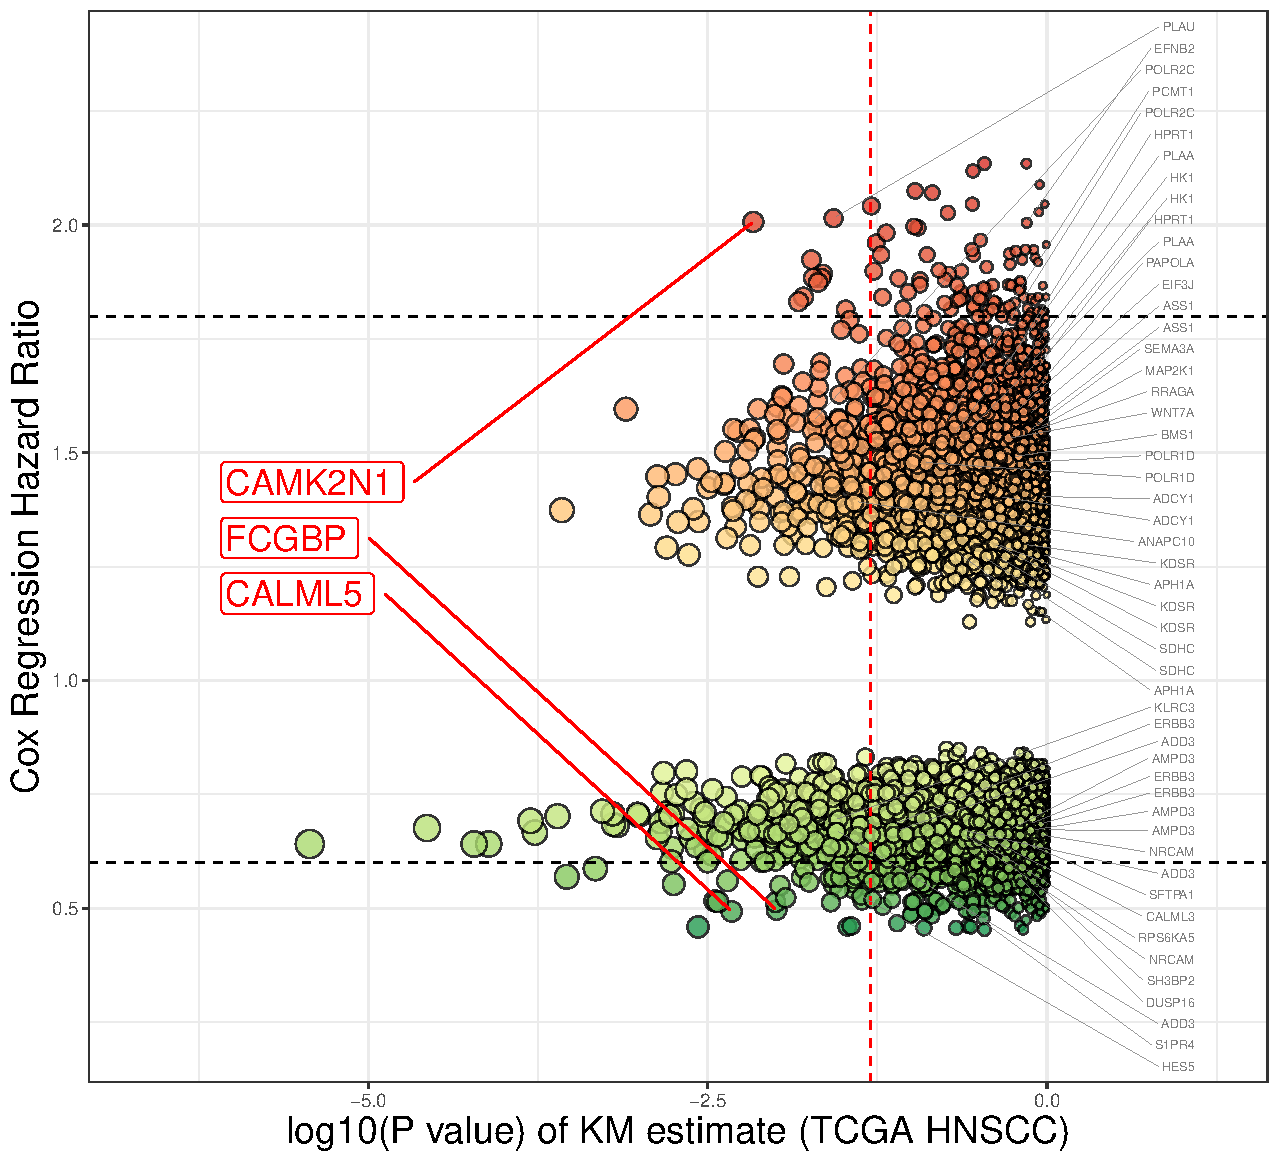
\includegraphics[width=\textwidth]{Rplot_TCGA_HNSCC_CoxHR_CAMK2N1_Bayes62_FDRKM.pdf}
        \caption{TCGA HNSCC cohort}
  \end{subfigure}
  \hfill
  \begin{subfigure}[b]{0.5\textwidth}
       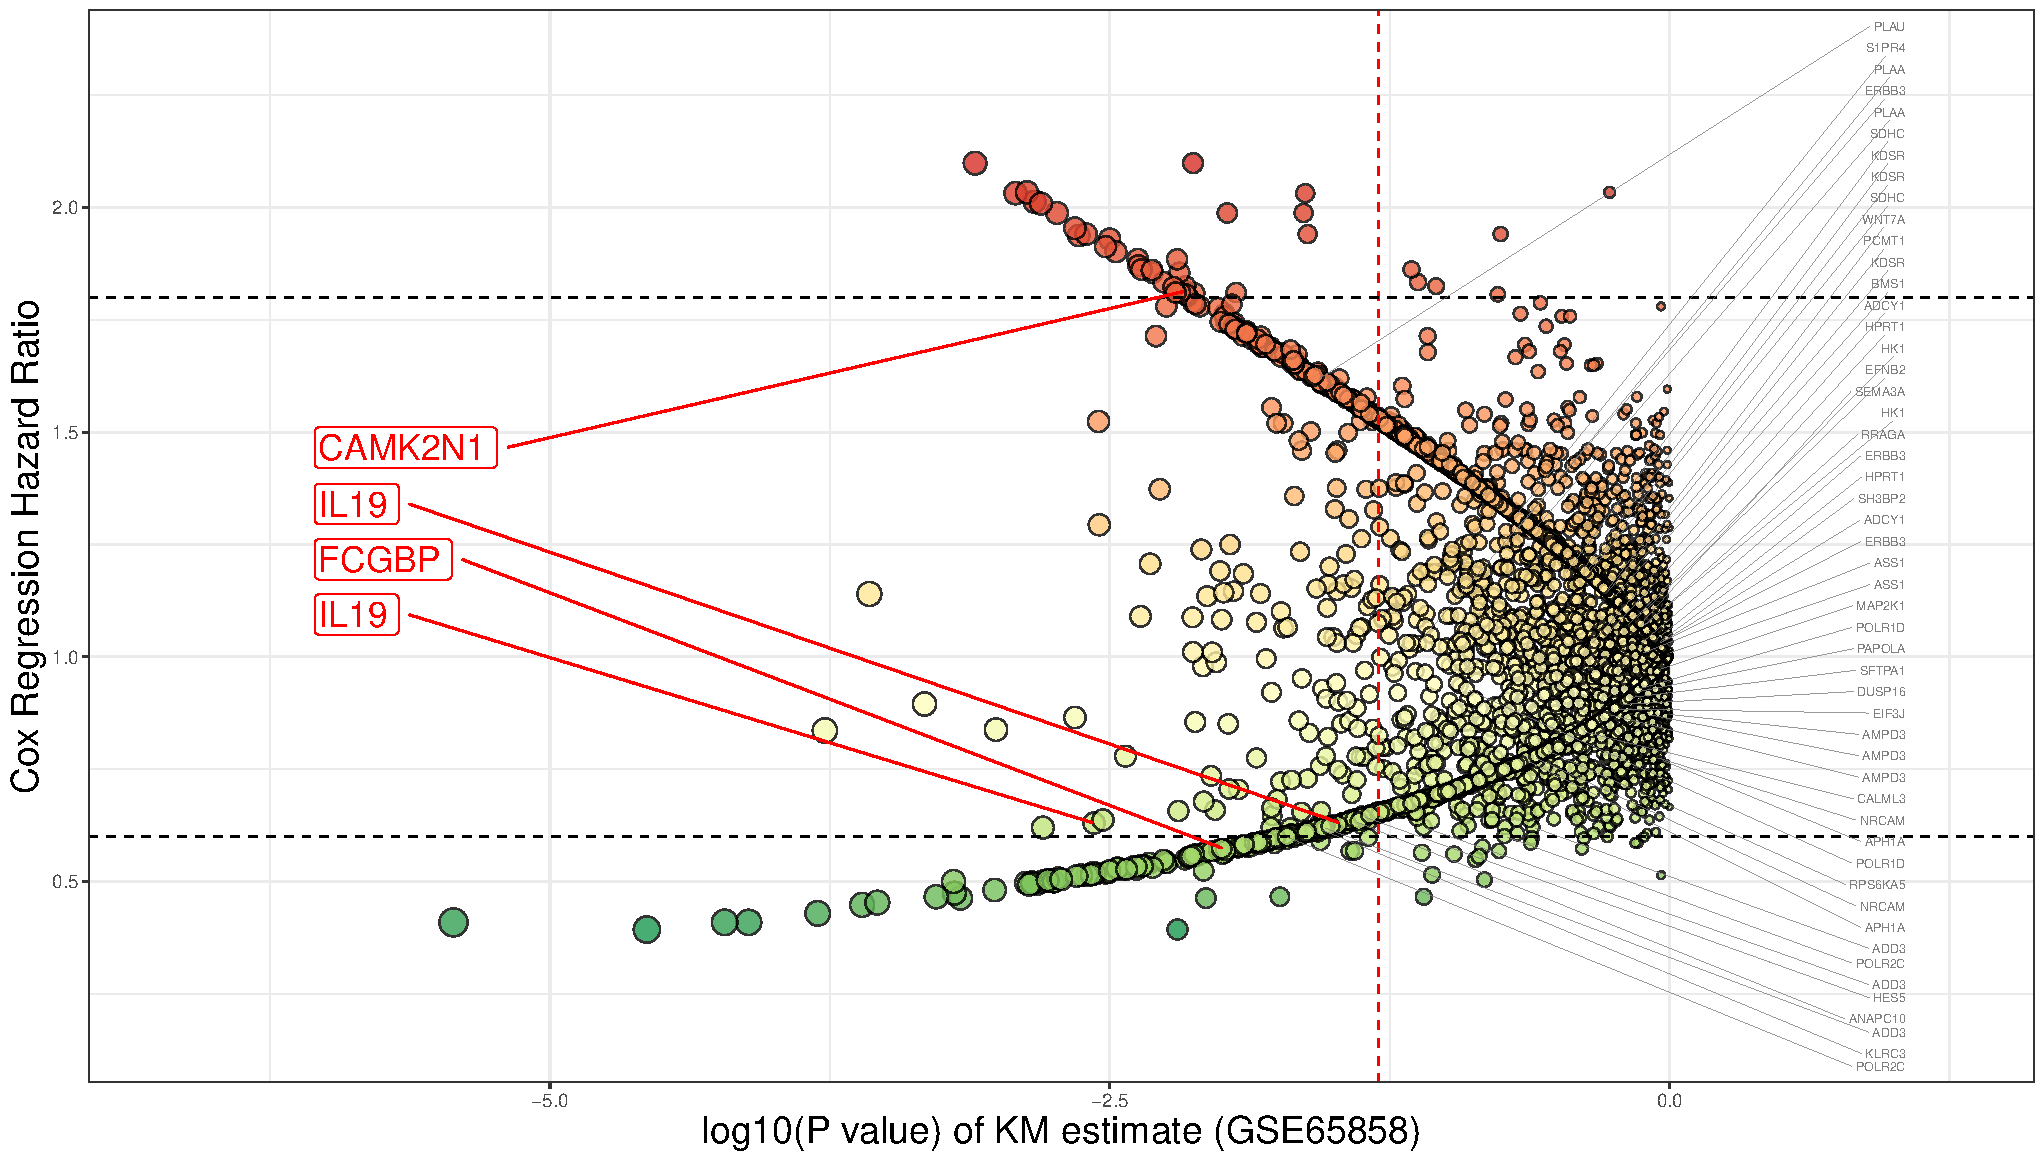
\includegraphics[width=\textwidth]{Rplot_GSE65858_HNSCC_CoxHR_CAMK2N1_Bayes62_FDRKM.pdf} 
       \caption{GSE65858 HNSCC cohort}
  \end{subfigure}
  \caption{The 62 genes (listed on the right), discovered by LASSO regression, distribute in (a) TCGA HNSCC and (b) GSE65858 HNSCC cohorts. \textcolor{red}{Red}-square marked genes are our 3 candidates: CAMK2N1, CALML5, and FCGBP.}
  \label{fig:Bayes62}
\end{figure}

% C-index = 0.68 in this model fitting
%accuracy for the classification in case-control study (or ROC, AUC)
% **** C-index, concordance index for survival data (with censoring)
%the Harrell concordance index (C-index) (1996) is the standard performance metric for model assessment in survival analysis with censored data.
%The predictive performances are computed in terms of C-index for the survival prediction. 

% Y-axis of the cross-validation error curve (red dotted line) (partial likelihood deviance)
%the left vertical line in the plot shows us where the cross-validation error curve hits its minimum.
%The final gene signature has been selected, including 4 genes, named HK1, EZR, RRAGA, and DUSP16 .; fentastic4
% lasso 就是要找出 coefficient of regression non-zero 的基因: selected features
LASSO calculate the (non-zero) coefficients of features, while the 62 genes hit the minimum of cross-validation error.
% in lambda 1se
%cv.mod$glmnetRes$lambda.1se
We have further limited gene selection (13 out of 62) by the most regularized model under cross-validation error within 1 standard deviation of the minimum.
According to their \textit{P} values (please see Table \ref{tab:signature4}), 
we found a gene signature, HK1, EZR, RRAGA, and DUSP16 to predict their survival impact on TCGA HNSCC cohort (please see Figure \ref{fig:signature4}).
DUSP16 has negative coefficient in the LASSO regression model, compatible with HR less than 1 in volcano plot of TCGA HNSCC.

% Please add the following required packages to your document preamble:
% \usepackage{graphicx}
% \usepackage[table,xcdraw]{xcolor}
% {\color[HTML]{FE0000} 0.002}  
% If you use beamer only pass "xcolor=table" option, i.e. \documentclass[xcolor=table]{beamer}
% Please add the following required packages to your document preamble:

\begin{table}[ht]
\centering
\caption{The most LASSO regularized logistic model under cross-validation. Genes with positive coefficient will increase the patient's risk, while negative reduce it.\\
    (\textcolor{red}{red}-marked logistic \textit{P} value $< 0.05$)}
\label{tab:signature4}
\begin{tabular}{lrr}
\textbf{Gene Symbol} & \textbf{Coefficients} &  \textbf{\textit{P} value} \\ \hline
\textbf{POLR2C}      & 0.870                 & 0.150                              \\
\textbf{EFNB2}       & 0.189                 & 0.521                              \\
\textbf{PLAU}        & -0.189                & 0.408                              \\
\textbf{HK1}         & 1.413                 & \textcolor{red}{0.002}       \\
\textbf{WNT7A}       & 0.211                 & 0.111                              \\
\textbf{HPRT1}       & 0.620                 & 0.113                              \\
\textbf{APP}         & 0.219                 & 0.538                              \\
\textbf{SC5DL}       & 0.262                 & 0.367                              \\
\textbf{EZR}         & 0.973                 & \textcolor{red}{0.017}       \\
\textbf{RRAGA}       & 0.925                 & \textcolor{red}{0.022}       \\
\textbf{S1PR4}       & -0.368                & 0.052                              \\
\textbf{DUSP16}      & -0.745                & \textcolor{red}{0.035}       \\
\textbf{SH3BP2}      & -0.606                & 0.107                             
\end{tabular}
\end{table}

%%%

\begin{figure}[ht]
%    \centering
  \begin{subfigure}[b]{0.3\textwidth}
    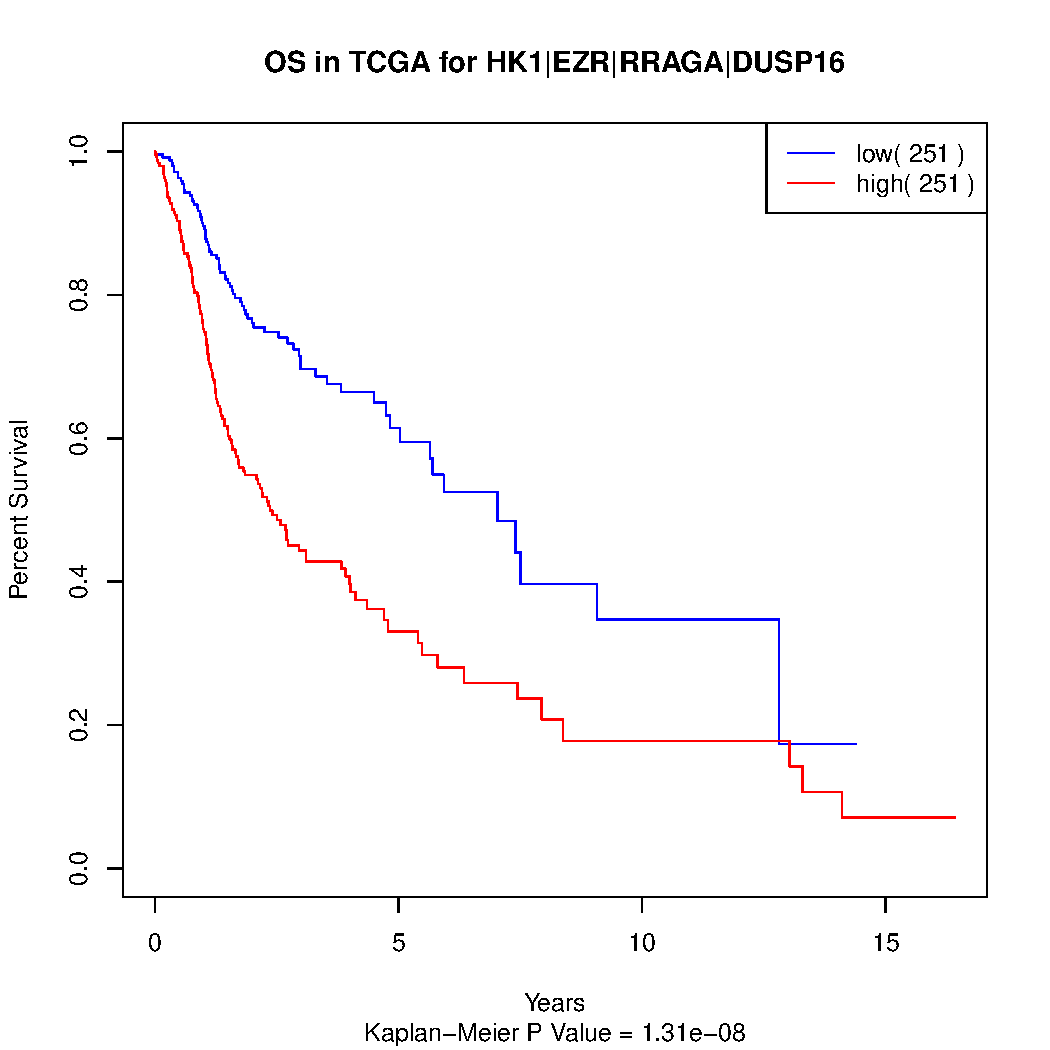
\includegraphics[width=6cm]{rplot_KMplot_HK1.pdf}
    \caption{Kaplan-Meier plot}
  \end{subfigure}
  \hfill
  \begin{subfigure}[b]{0.5\textwidth}
    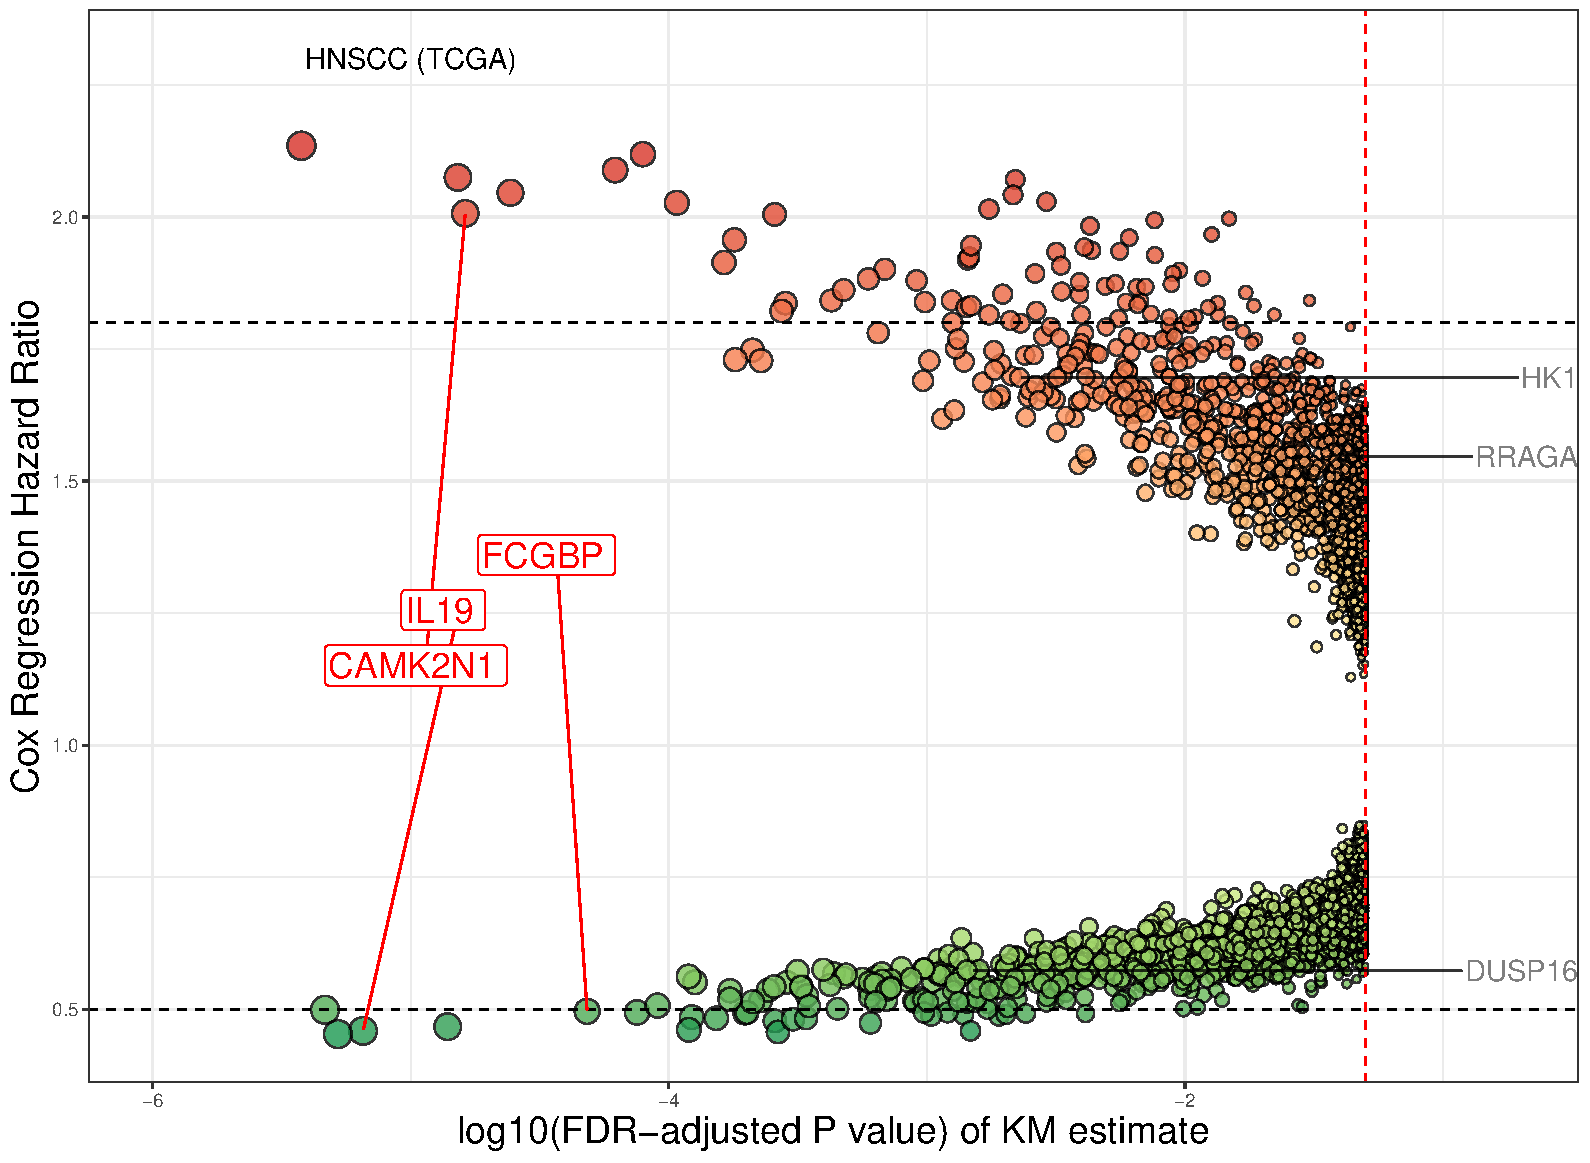
\includegraphics[width=8cm]{Rplot_TCGA_HNSCC_CoxHR_CAMK2N1_signature4_FDRKM.pdf}  
    \caption{Volcano plot}
  \end{subfigure}
%However, # 4 gene signature: #### 
%# "EZR" has \textit{P} value $>0.05$
  \caption{(a) Overall survival in TCGA HNSCC for a gene signature including HK1, EZR, RRAGA, and DUSP16 (Kaplan-Meier \textit{P} value = \num{1.31e-6}); (b) Those genes (listed on the right side) have not significant hazard ratio (HR) if calculated individually (EZR is not shown on volcano plot due to it's Kaplan-Meier \textit{P} value $>0.05$)}
    \label{fig:signature4}
\end{figure}



In conclusion, we might build a Lasso regression model with LASSO regularization to maximize the use of continuous gene expression values (without the need of a cutoff).
The gene signature integrating multiple genes is also a good approach for biomarker discovery.
However, the resulting candidates could be influenced by proper "gene interaction network" applied for model building.
% gene signature
RLassoCox package works on the basis of gene signature that are related to a grouping structures with similar biological functions tend to have similar expressions. 
RLassoCox utilizes Kyoto Encyclopedia of Genes and Genomes (KEGG) network\cite{Simon2011} as the reference of gene interaction networks, constructed by the R package "iSubpathwayMiner".
% data(dGMMirGraph) # The KEGG network constructed by the R package iSubpathwayMiner.

%https://bmcbioinformatics.biomedcentral.com/articles/10.1186/s12859-020-03544-z
%https://bmcbioinformatics.biomedcentral.com/articles/10.1186/s12859-021-04040-8
%or
% PCA of gene signature => L1/L2 penalized Cox model; L1-penalized (Lasso) Cox proportional hazard regression model (R package glmnet)
%x Statistical methods: Development of a 13-gene signature prediction model for survival in HPV-negative OSCC patients.
%To build a prediction model for OSCC-specific survival unique to the patients with HPV-negative OSCCs\cite{Lohavanichbutr2013}.

%or \cite{Zhao2018} Prognostic gene signature:\\ % https://www.hindawi.com/journals/jir/2020/5494858/

%The risk score for each HNSCC sample was calculated based on the IRGP prognostic signature using the following formula:\\[0.5cm]
%risk score = $expression_{gene1} \times \beta_{gene1} + expression_{gene2} \times \beta_{gene2} + ... + expression_{geneX} \times \beta_{geneX}$\\

%*** how to do? ROC
% https://compgenomr.github.io/book/assessing-the-performance-of-our-model.html
%In addition, receiver operating characteristic (ROC) analysis was used to estimate the predictive power of this signature\cite{Huang2019}.
%---

%, in which $X$ was the number of IRGPs and $\beta$ was coefficient value for each IRGPs. Taking the median value of risk score as the threshold, we divided all the HCC samples into high-risk or low-risk groups. The accuracy and sensitivity of survival prediction based on the risk score were verified by receiver operating characteristic (ROC) curve analysis and determined by the value of area under the curve (AUC) in 1, 3, and 5 years. Kaplan–Meier (KM) survival curves analysis () was used to analyze the over survival (OS) of the high-risk and low-risk groups. We then integrated IRGPs with existing clinical and pathologic features for multivariate Cox regression analysis. Tumor TNM, stage, grade, age, and body mass index (BMI) were regarded as continuous variables. The association between IRGPs risk score, clinical, and pathologic features was determined by KM analysis. Prognostic risk models of tumor TNM, grade, age, and stage were constructed. Subsequently, a Cox proportional hazards regression model was constructed by combined the Tumor TNM, grade, age, stage, and risk scored. The R package rms was used to compare these models with the IRGP prognostic signature. Concordance index (C-index) was used to assess the accuracy of the prognostic biomarkers. Also, the comparison between IRGPs and clinical/pathologic features was performed by forest and nomogram plots to determine the effectiveness of the prognostic value. The statistical difference of IRGPs in the clinical/pathologic features was compared using the Kruskal–Wallis test.

 
%***Ultimately, the gene expression profile from the GEO and OSCC cell lines and tissues were used to verify these primitive biomarkers. In addition, a combination of two or more biomarkers was performed to predict OSCC overall survival according to the gene expression in TCGA\cite{Huang2019}.

%** or using %Rplot_GSE65858_CoxHR1.5_top19.pdf
%KM estimate and Cox modeling to yield a geographically closed gene cluster:
%CAMK2N1, TIMM10, TNFAIP6, SPP1, ADAMTSL2.

\end{MyColorPar}
%
\clearpage

\subsection*{2-6}
%(OK)
\subsubsection*{[Minor comments]}
The background should be revised extensively. For example, the description of the linear model should be removed. X1...Xn should be removed. 
More introduction to how other researchers used TCGA to find expression biomarkers should be presented. 
Detailed introduction of TCGA-related tools should be removed or moved to Methods.
In line 154 paragraph, what does unclean data mean, missing values or zero expression? The three challenges are not “challenges” at all. The authors exaggerated the difficulties here.
In Figure 1, the diagram should have direction. 
The file names are not interesting. RNAseq (20500 genes) should be gene expression values (20500 genes)
In Figure 2, unlabeled scales on the x-axis.


%
\begin{MyColorPar}{blue}
Answer

%(OK x3)
% (ok) minor comments1
We appreciate the reviewer for the critical comments and thanks for the agreement of our workflow in cancer research.
The description of the linear model has been removed. 
Detailed introduction of TCGA-related tools has been moved to the Materials and Methods.
We made a new "Figure 1" with clear direction of the workflow.
And the "gene expression values (20500 genes)" replaced the "RNAseq" (it is shown here as Figure \ref{fig:figure1} on page \pageref{page21}).
In "Figure 2", the ticks and labels on the x-axis were corrected (please also see Figure \ref{fig:figure2} on page \pageref{page22} in this file).\\[0.5cm]

%%% new figure 1; fig:figure1

%\subsubsection{Figure 1:h}
\begin{figure}[hbt!]
\centering
%\widefigure
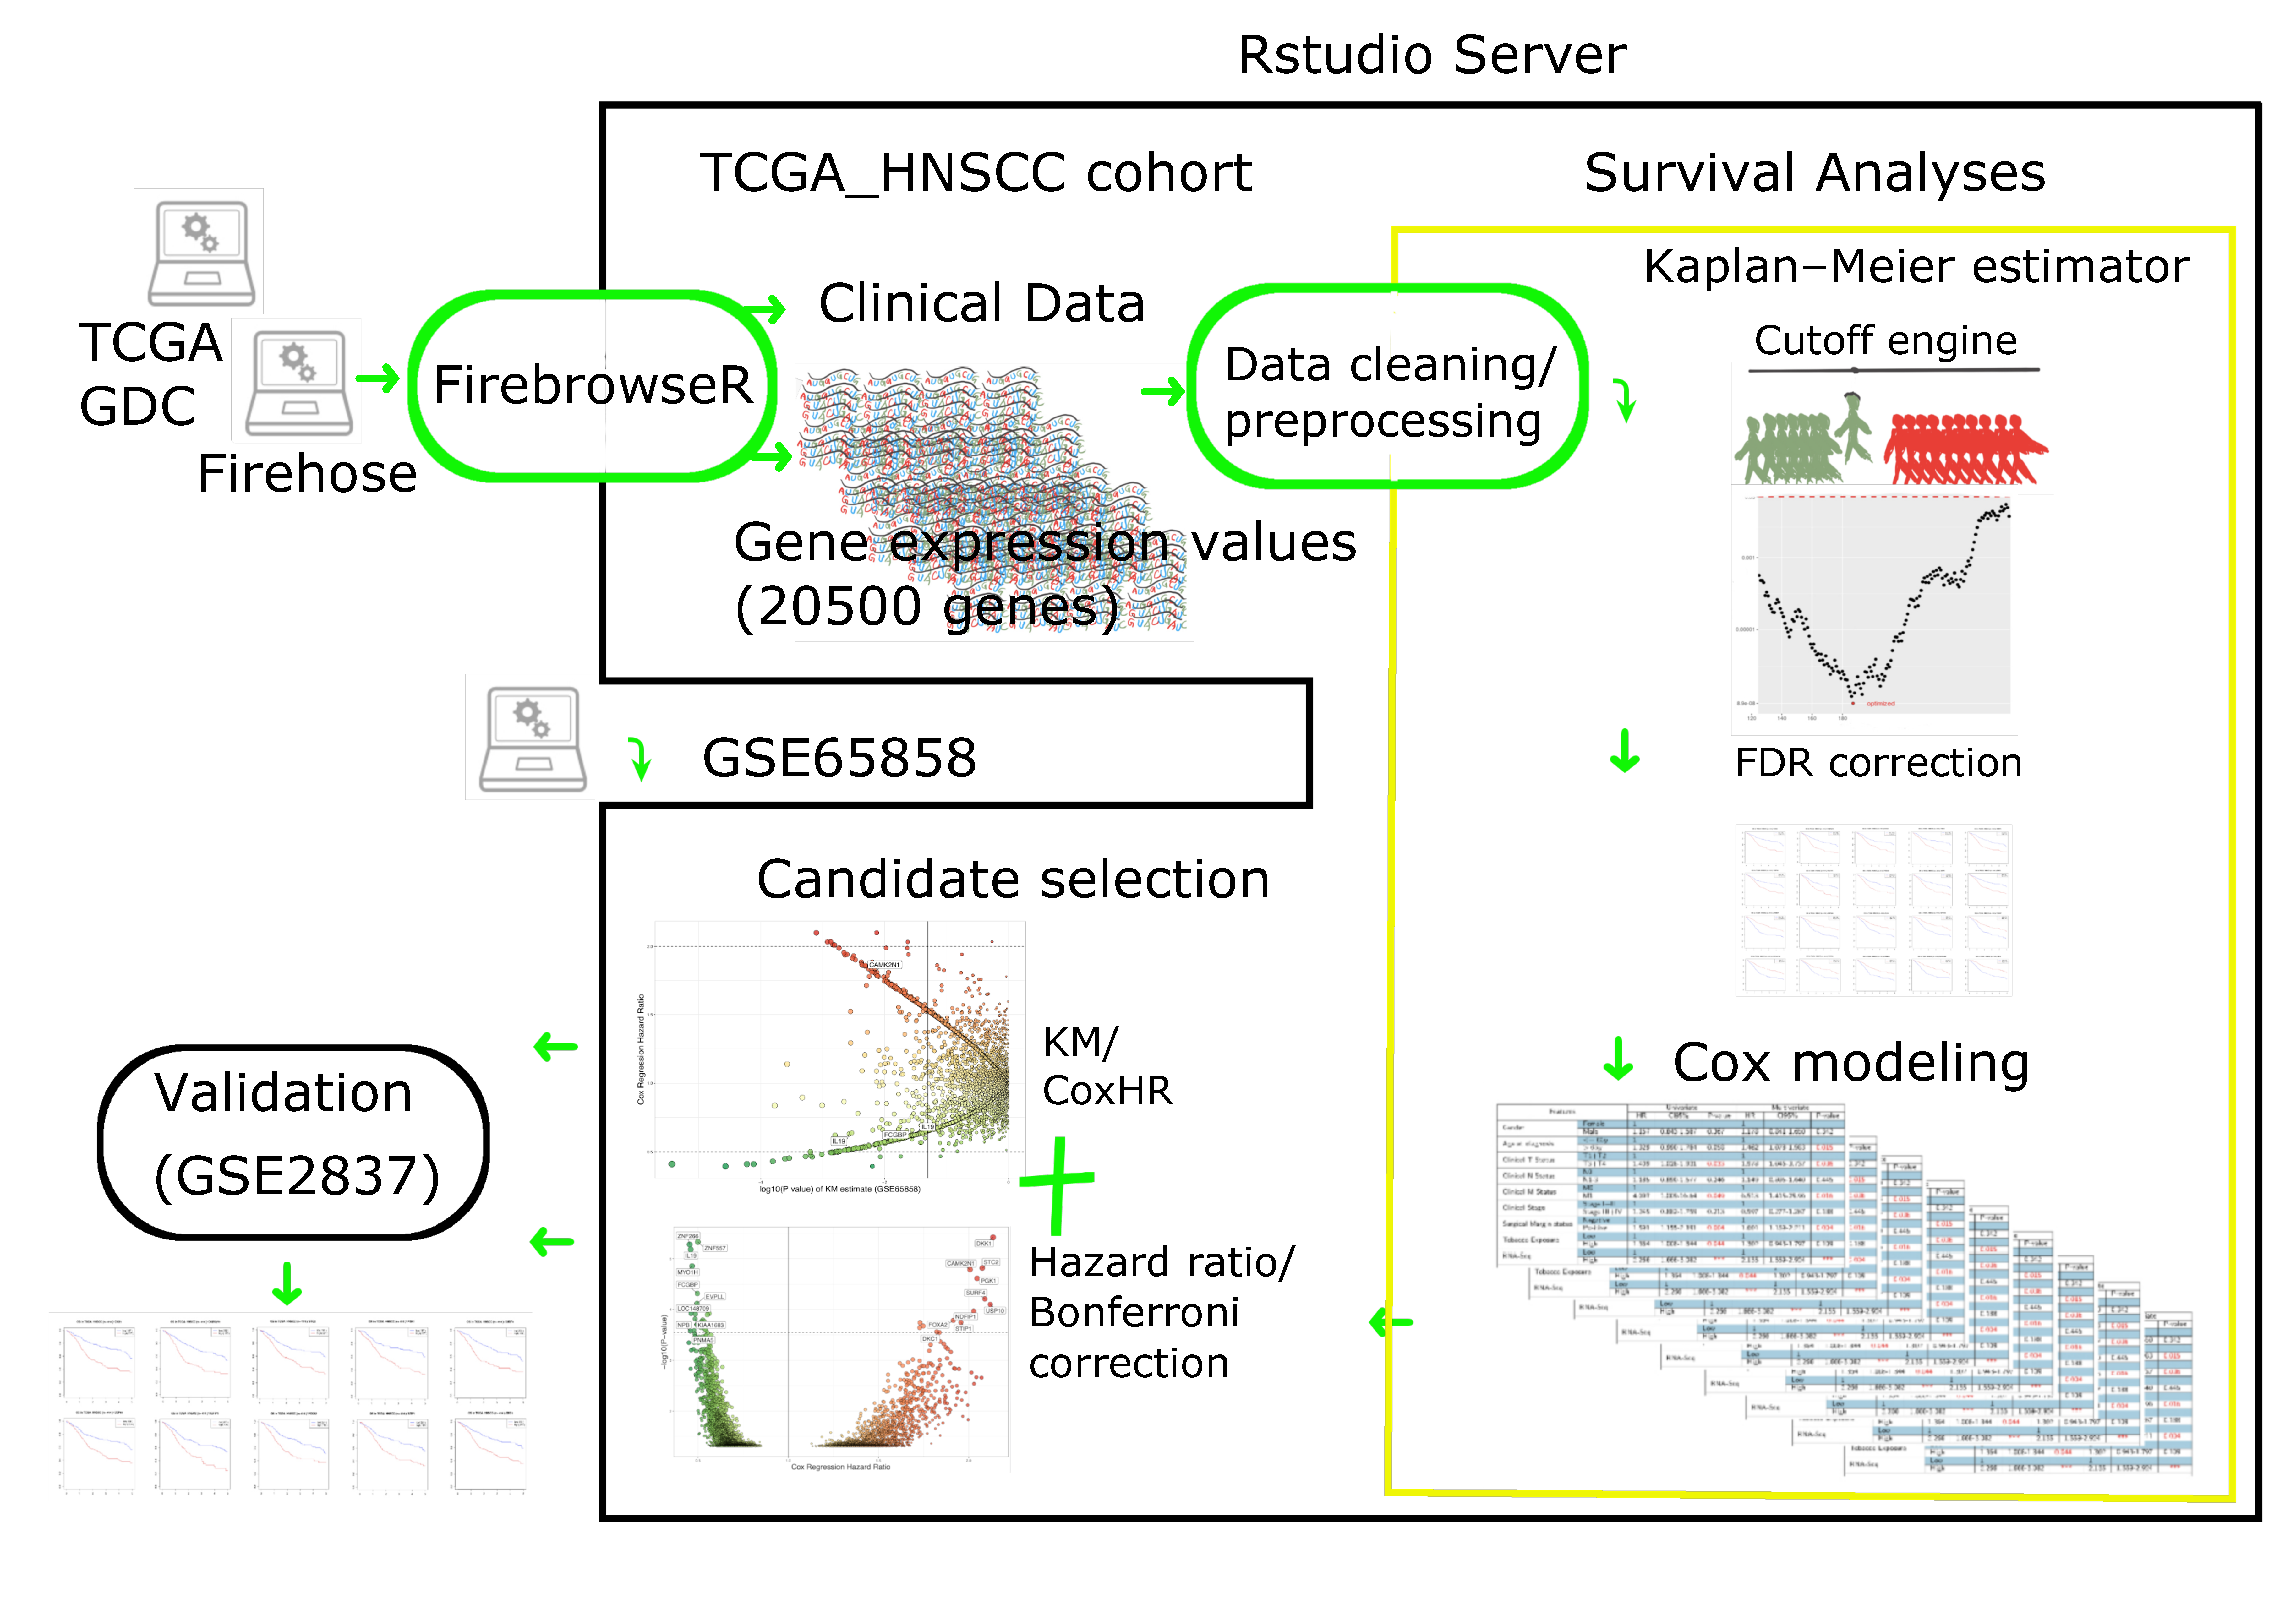
\includegraphics[width=14cm]{Figure_1_manuscript_workflow} % .PDF is better than .png
%, height=8cm
%\caption % , step 1 (\textcolor{blue}{blue line}: main procedure) and step 2 (\textcolor{orange}{orange line}: analysis export).
%Step 3 (purple line: dealing with surgical margin).
\bcaption{A workflow of \acrshort{hnscc} biomarker discovery}
{The workflow includes data retrieval from TCGA GDC data portal, data process with merging and cleaning, then performing the survival analyses (within \textcolor{yellow}{yellow} square). The Cutoff engine (in R script: cutofFinder\_func.HNSCC.R, a serial cut for grouping patients with \textcolor{asparagus}{low} or \textcolor{red}{high} expression of a specific gene, to yield a collection of \textit{P} values; please see Materials and Methods section for details) might calculate all possible Kaplan-Meier \textit{P} values (corrected by \acrlong{fdr}, FDR, method) to find the optimal cutoff value of gene expression for subsequent Cox modeling.
The candidate selection performs (1) dissecting and selection of candidate genes by further Bonferroni adjusted \textit{P} values as well as a hazard ratio of Cox model, based on the results from the survival analyses;
(2) survival analyses of the other HNSCC dataset (GSE65858) using Kaplan-Meier estimate (with FDR correction) and Cox modeling.\\
The biomarker candidates were a consensus result of TCGA and GSE65858. 
%The selected genes were validated by third HNSCC cohort (GSE2837).\\
(HNSCC: head and neck squamous cell carcinoma; TCGA: the Cancer Genome Atlas; RNA-Seq: RNA sequencing; GDC: Genomic Data Commons.)}
\label{fig:figure1}
% Description:1) FDR correction of Kaplan-Meier \textit{P} values during Cutoff finding; and 2) Bonferroni correction of Kaplan-Meier \textit{P} values after Cox modeling for candidate selection.

\label{page21}
\end{figure}

%%% new figure 2; fig:figure2

%\subsubsection{Figure 2:h}
\begin{figure}[hbt!]
\centering
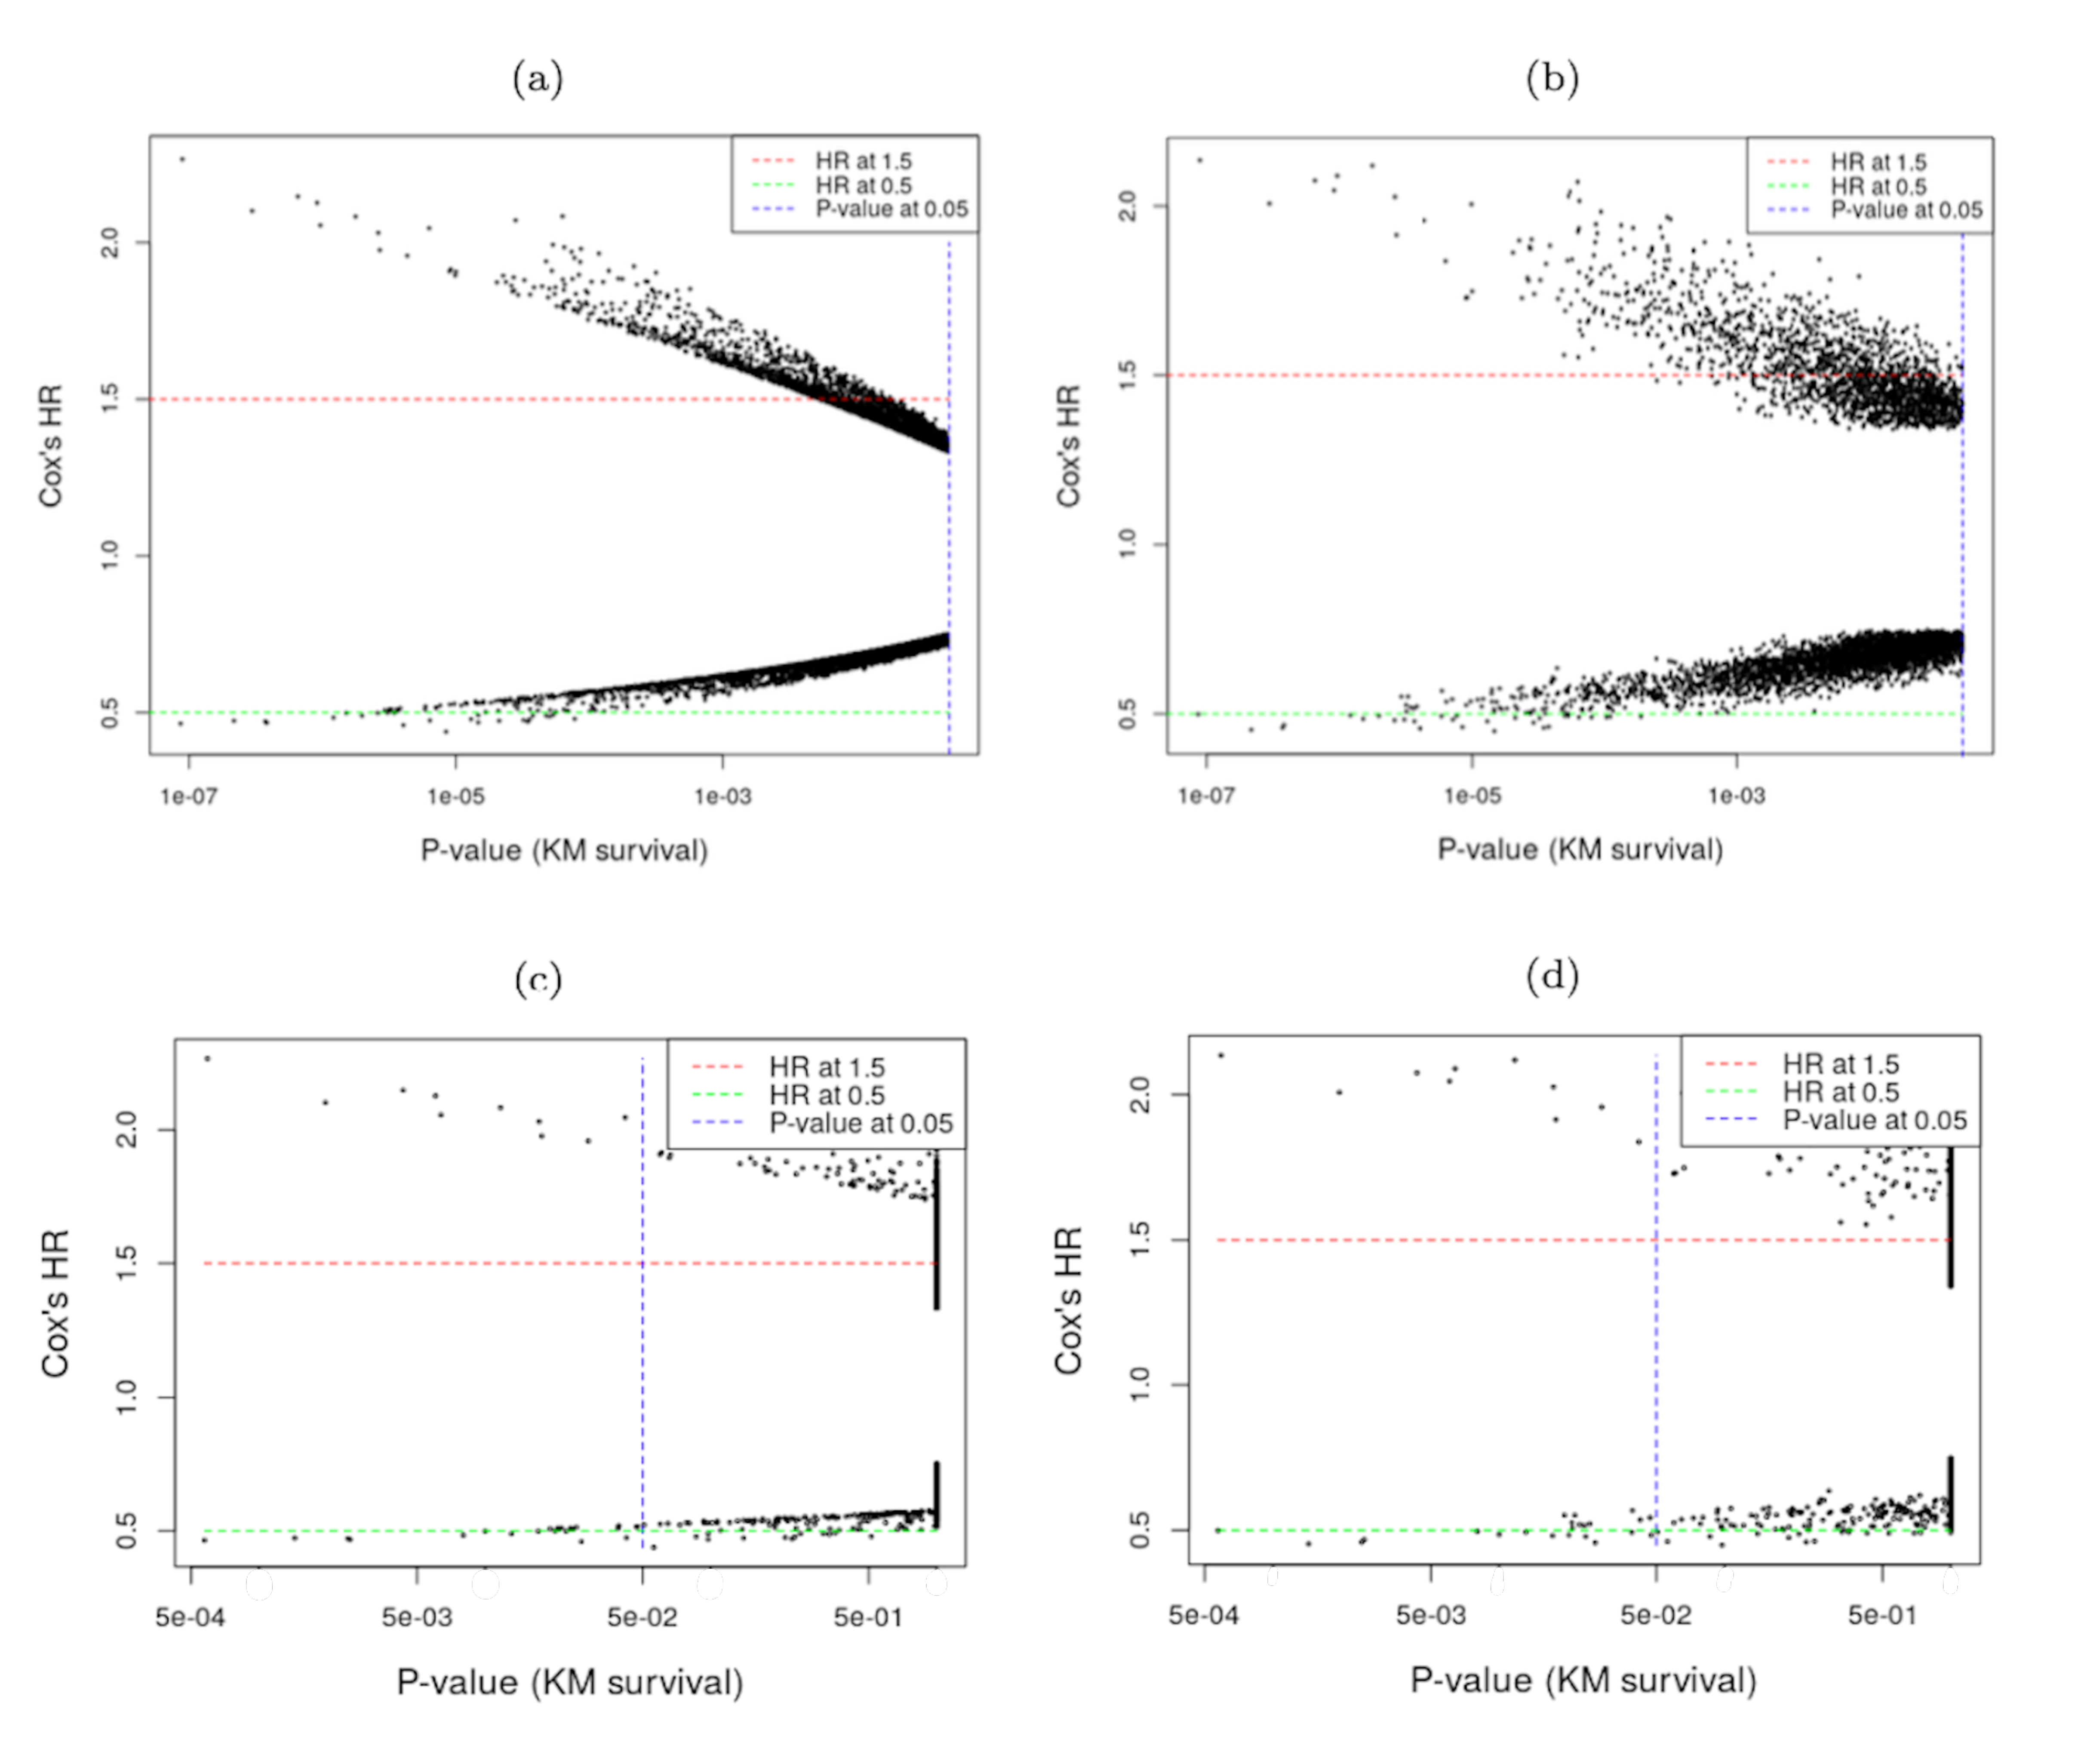
\includegraphics[width=14cm]{Figure2.pdf}
\bcaption{The initial progress of candidate selection from TCGA \acrshort{hnscc} cohort.}{The \textit{P} values of Kaplan-Meier survival is one of the selection criteria.
The effect size is estimated by Cox's hazard ratio.
Initial trial step: (a) univariate HR versus \textit{P} value; (b) multivariate HR versus \textit{P} value.
After stringent criteria by Bonferroni-adjusted \textit{P} value, and the Cox's HR, few top-ranked genes are shown in
(c) univariate HR versus Bonferroni-adjusted \textit{P} value; and (d) multivariate HR versus Bonferroni-adjusted \textit{P} value.\\
(TCGA: \acrlong{tcga}; HR: hazard ratio)}
\label{fig:figure2}
\label{page22}
\end{figure}


%%
\begin{MyColorPar}{black} % minor comment2
\subsubsection*{[Minor comments]}

More introduction to how other researchers used TCGA to find expression biomarkers should be presented in the Introduction section.
\end{MyColorPar}

Answer

We placed more descriptions about researcher's work using TCGA to find expression biomarkers in the Introduction section.
% ok
The paragraphs marked in \textcolor{red}{Red} on page 3 (line 98 to line 123) are the part of the manuscript that has been revised. Also, it is shown here in the following paragraph.\\[0.3cm]


\begin{MyIndent}
\begin{MyColorPar}{red}
% inserted at \subsubsection{From TCGA to expression biomarkers}

% EdgeR
% GEPIA2: most differential survival gene = pvalueTex
"
%\subsubsection{from TCGA to expression biomarkers} 
%%% how other researchers used TCGA to find expression biomarkers
Usually, researchers developed an in-house workflow of gene expression analysis of TCGA data to find HNSCC biomarkers.
%Workflow of GDCRNATool
% reference https://www.biostars.org/p/153013/
%Tutorial: Survival analysis of TCGA patients
%integrating gene expression (RNASeq) data.
%Why would you want to do survival analysis based on gene expression data? Well, let's say you
% **** DEGs is a different concept with cutoff finding survival analysis of individual gene expression
They have several genes that are differentially expressed between tumor and normal samples.
It would be helpful to show that alteration in gene expression correlates with phenotypes of HNSCC.
%%% https://www.biostars.org/p/153013/
%% download data with offline analysis
%Usually, investigators could download the TCGA data in order to analyze and find expression biomarkers.
% https://groups.google.com/forum/m/#!msg/ucsc-cancer-genomics-browser/YvKnWZSsw1Q/3IAkkEMyFa4J
% from Mary Goldman and Jing Zhu, UCSC Cancer Browser
% https://genome-cancer.ucsc.edu/
%Here are the summarized techniques currently used: from 2000 to 2017\cite{Tonella2017a}
%Gene expression profiling is applied for HNSCC to help in early diagnosis, prediction of recurrence or metastasis, prediction of prognosis or response to some therapies.
% Rstudio\cite{Loraine2015a}
Some researchers\cite{Loraine2015a}\cite{Tonella2017a}\cite{Zhao2018}\cite{Li2018a}\cite{Huang2019}\cite{Shen2019}\cite{Schmitt2019}\cite{Xu2021a} tried to find \acrfull{degs} of the HNSCC samples at both genotypic and phenotypic levels (without survival information) for biomarker discovery.
Gene expression data was downloaded from the TCGA or Gene Expression Omnibus (GEO) database (e.x. GSE117973\cite{Schmitt2019}, HIPO-HNC cohort has n = 87).
% IRB: Patient samples were obtained under the protocol S-206/2011, approved by the Ethics Committee of Heidelberg University, with written informed consent from all participants.
%e.x. GSE30784: 167 HNSCC samples and 45 normal controls). 
They employed the Database for Annotation, Visualization, and Integrated Discovery (DAVID, available at https://david.ncifcrf.gov/) to obtain information for Gene Ontology (GO), including biological processes, the cellular component, and molecular function. 
The Kyoto Encyclopedia of Genes and Genomes (KEGG) pathway analysis was also used to annotate the potential functions.
%Subsequently, comprehensive bioinformatics analysis incorporating gene ontology (GO), Kyoto Encyclopedia of Genes and Genomes (KEGG),
The protein-protein interaction (PPI) network was conducted by STRING (available at https://string-db.org).
The pathway enrichment analysis of \acrshort{degs} was also performed by DAVID, String, or Cytoscape software programs\cite{Huang2019}\cite{Shen2019}.
Li\cite{Li2018a} and his colleagues made an R package (GDCRNATool) for the implementation of those workflows on gene expression analyses of the TCGA.
%The DEmRNAs were enrolled in a protein-protein interaction (PPI) network through the STRING database (https://string-db.org/) with a confidence score $> 0.9$, and the PPI network was visualized in Cytoscape (Version 3.7.1) software. Moreover, genes with degree $>= 25$ were selected as hub genes. Subsequently, module analysis (16) of the PPI network was performed using the Molecular Complex Detection (MCODE) tool of Cytoscape software, and GO and KEGG analysis of the modules was carried out using the DAVID database.
%a validation set and
%Then, Kaplan–Meier survival curves along with a log-rank test were applied to select candidates\cite{Xu2021a}.
Xu and his colleagues\cite{Xu2021a} also used Kaplan–Meier survival curves with a log-rank test, and univariate Cox regression to screen prognostic factors.
The gene expression was used to select the preliminary biomarkers with a significant impact on patients' overall survival (\textit{P} value $< 0.01$).
%By integrated bioinformatics analysis, including protein_protein interaction (PPI) network, Gene Ontology (GO) enrichment, and Kyoto Encyclopedia of Genes and Genomes (KEGG) pathway enrichment analyses. The PPI network was established using the Search Tool for the Retrieval of Interacting Genes (STRING) and Cytoscape software.
The candidate genes were validated via the Gene Expression Profiling Interactive Analysis tool (GEPIA1/2 database using TCGA datasets, developed by Zefang Tang and his colleagues\cite{Tang2017a}\cite{Tang2019}
%, datasets from projects of the TCGA and the Genotype-Tissue Expression, GTEx
), GEPIA2021\cite{Li2021} (available at http://\\gepia2021.cancer-pku.cn/), or the Human Protein Atlas (HPA) website.
% GTEx https://gtexportal.org/home/; non-disease 54 tissues/organs
% GEPIA1/2 contact us: tangzefang@pku.edu.cn
Finally, the gene expression profile from the GEO and HNSCC cell lines and tissues were used to verify these biomarkers.
"
%DEGs to hub: The 230 differentially expressed genes and 12 hub genes were subjected to functional and pathway enrichment analyses. Then hub genes for survival analyses.

% Cox Risk Regression Establishment and Validation with lncRNA data
%HNSCC samples were randomly divided into a training set and a validation set. Univariate Cox regression was used to select prognosis-associated genes (\textit{P} value $< 0.05$). Subsequently, we performed "Least Absolute Shrinkage and Selection Operator" (LASSO) Cox regression model to do feature selection\cite{Tibshirani1996};
%establish a prognostic risk score model, and the penalty regularization parameter lambda ($\lambda$) was chosen through cross-validation with an n-fold equal to 10 by using the R package glmnet (21). 
%https://glmnet.stanford.edu/articles/glmnet.html
%Lambda.min was identified to pick out the variables. According to these variables, a stepwise regression was performed to establish the Cox model. 
%Least Absolute Shrinkage and Selection Operator (LASSO) cox regression model along with 10-fold cross-validation




%Biomarkers Screening and Validation
%The status and survival time of HNSCC patients were extracted. Subsequently, the mRNA was enrolled in the PPI and ceRNA networks, and lncRNA and miRNA identified in ceRNA were selected for screening biomarkers. 


%


%%%%%%%%%
\end{MyColorPar} % red
\end{MyIndent}

% ok
\begin{MyColorPar}{black} % minor comment3
\subsubsection*{[Minor comments]}
%%%***[latex line 410]

In line 154 paragraph, what does "unclean data" mean, missing values or zero expression? 
The three challenges are not "challenges" at all. The authors exaggerated the difficulties here.\\[0.3cm]
\end{MyColorPar}

Answer

% 不要誇大說明 謙虛道歉
We apologize for exaggerating the difficulties of our workflow.
% ok
The paragraphs marked in \textcolor{red}{Red} on page 11 (line 282 to line 310) are the part of the manuscript that has been revised. Also, it is shown here in the following two paragraphs.


\begin{MyIndent}
\begin{MyColorPar}{red}
%%%
"
There are two essential points of biomarker discovery from survival analysis of the TCGA HNSCC dataset.

First, although \acrshort{tcga} genomics data were harmonized, 
% three things were found during our investigating and data cleaning:
the pre-processing of TCGA RNA-Seq in our workflow has been done as follows: 
\begin{outline}
\1 HNSCC samples without complete clinical information have been removed;
\1 Null expressed genes in more than 30\% of the HNSCC samples have been excluded; % or 50\%
\1 Updated number of protein-coding genes in the TCGA HNSCC is 20500.
\end{outline}
After investigation of mRNA expression dataset obtained through NCI's Firehose API, we found that expression value of two genes (gene ID: 9906 and gene ID: 728661) was saved together under the entity of gene symbol "SLC35E2".
The expression file of SLC35E2 has almost double in size than those of SLC35E1 or SLC35E3.
% http://gepia2.cancer-pku.cn/#survival is SLC35E2; 證明 TCGA has error
% [line 1549]
%HNSCC.mRNA.Exp.SLC35E2.Fire.Rda
%[line 1654]
%for gene correction (20499 to 20500) from SLC35E2 to 2 genes:
%NCBI Reference Sequences (RefSeq) National Center for Biotechnology Information Reference Sequence (NCBI) RefSeq Release 38 (November 7, 2009) 
According to the Human Gene Database (available at https://www.genecards.org/Search/Keyword?\\queryString=SLC35E2), SLC35E2A (Gene ID: 9906) and SLC35E2B (Gene ID: 728661) should be the correct entities for the TCGA HNSCC dataset.
% https://www.ncbi.nlm.nih.gov/gene/?term=(SLC35E2)+AND+%22Homo+sapiens%22
% keyword: (SLC35E2) AND "Homo sapiens" 
SLC35E2 is the previous symbol of SLC35E2A (reference at https://www.genenames.org/data/gene-symbol-report/\\\#!/hgnc\_id/HGNC:20863).
Thus, we made reassignment of the expression value of SLC35E2A and SLC35E2B and updated the number of protein-coding genes in this TCGA HNSCC dataset from 20499 to 20500.
% updated on 18-May-2021 then 01 July 2021


%Second, we find a way to determine candidates from the expression level of 20,500 human protein-coding genes\cite{Clamp2007}.

% risk of *** Answer 2-3 併入此
%Second, trying to find an optimal cutpoint of that \acrshort{rna} expression data to maximize candidate mining coverage, this strategy could identify more but sometimes weak "biomarkers".
%We have checked this issue in detail (in the Discussions section).
%Thus, the false positives and adjustment of multiple comparisons should be corrected by \acrfull{fdr}.
%Furthermore, validation of those candidates is required in the other independent dataset.
% in larger patient populations.% in larger patient
%warrant.

% dissection
%ZSWIM2\_archive.Rda % 其實最困難的在於 unknown error (ZSWIM2) 
Second, we analyzed the error log during the cutoff finding and Cox modeling, 
the result shows that program running could be halted by several technical problems.
These include:
\begin{outline}

\1 32.2\% event has "one group" issue in confusion matrix of Chi-square test in Cox regression;
\1 21.05\% error occurs by "one group" issue in log-rank test (survdiff or survdiff.fit function in R package "survival") in Kaplan-Meier estimate;
%1) ok [1] "[ 4 / 20083 ] Generating median-cut KM plot of A1BG"
%Error in survdiff.fit(y, groups, strata.keep, rho) : at A1CF
% error at 16115 gene ""; why? 518 values all are -0.04203 at T
%  There is only 1 group 
%This is because of skewed distribution of the expression value. 
% 67/518 =  13% cases >1, while 450 (87%) cases = -0.30949; so median is -0.30949; 
% all cases belong to >= median => 改為 > median 即可
% 2) % survfit 16114 has data set has no non-missing observations: NA's 113/518 cases
% median = NaN :-); 
% solved by cutoff <- median(gset_OS_mRNA2[, i], na.rm = TRUE)
% and NaN imputation as median
\1 0.78\% has unknown reason (so those 159 genes has been excluded in our workflow).
\end{outline}
These technical problems could not be detected prior to program running.
It might be due to skewed distribution of the expression value or even random error in 20500 RNA-Seq data. % heterogeneity
"

%# deal with return(1), return(2) and return(3) errors, try to solve it
%32.2\% error01, ZSWIM2 skip from contingencyTCGA(), it is one group issue in Melt() function.
%21.05\% errors in  one group in survdiff on KM cutofFinder_func.R.
%0.78\%(159 genes) for unknown reason
%# _marginS_
%n_percent_Bonferroni <- ZSWIM2_2$Freq[1]/sum(ZSWIM2_2$Freq) # 0.4593171 -> 0.4581951
%error01_sample <- which(ZSWIM2$X3==1) #  32.2\% error01: "ZSWIM2 skip from contingencyTCGA()"): one group issue in Melt()
%# => *** re-run
%error02_sample <- which(ZSWIM2$X3==2) # 14.2\% error02: There has only one group in survdiff.
%error03_sample <- which(ZSWIM2$X3==3) # 6.85\% error03: There has only one group in survdiff on KM cutofFinder_func.R.
%#=> Test for difference (log-rank test is multiple Chi-square alone survival time) with P-value; or Test for different KM curve between two groups (seperated by PMM1_median 0 vs 1)
% error05_sample <- which(ZSWIM2$X3==5) # 0.78\%(159 genes) error05: for why?



\end{MyColorPar} % end of red
\end{MyIndent}

\end{MyColorPar} % end of blue answer 2-6
% the end of response rebuttal %%%%%%%%%%%%





%\reftitle{References}

% Please provide either the correct journal abbreviation (e.g. according to the “List of Title Word Abbreviations” http://www.issn.org/services/online-services/access-to-the-ltwa/) or the full name of the journal.
% Citations and References in Supplementary files are permitted provided that they also appear in the reference list here. 

%\externalbibliography{yes}
%\bibliography{your_external_BibTeX_file}
\bibliographystyle{unsrt} %model1-num-names}
\bibliography{TCGA_margin_cutoff.bib, Deep_Learning.bib}


%\section{end_document}
\end{document}

%%%%%%%%%%%%%%%%%%%%%%%%%%%%%%%%%%%%%
\pagebreak

%\section*{Response to Reviewer 3 Comments}
%Response to Referees} % rebuttal
We much appreciate the reviewers for their helpful suggestions and critical comments on our manuscript. The detailed point-by-point reply to the reviewer's comments are as follows (marked as \textcolor{blue}{blue}). 
%Moreover, the revised portions in the manuscript are indicated in \textcolor{red}{red}.


%\subsection*{Comments from the reviewer \#3}

Round 1:
%Must be improved:
%Is the research design appropriate?
%Are the results clearly presented?
Are the conclusions supported by the results?

Only computer computing in this research to support 20 candidate biomarkers, DKK1, CAMK2N1, STC2, PGK1, SURF4, USP10, NDFIP1, FOXA2, STIP1, DKC1, as well as ZNF557, ZNF266, IL19, MYO1H, FCGBP, LOC148709, EVPLL, PNMA5, IQCN (previous name as KIAA1683), and NPB, are all heavily associated with the prognosis of OS.

There is little information provided. The authors should provide more evidence to support this article.

Round 2:
The authors still did not provide any experiment results that support the finding of the manuscript.



\begin{MyColorPar}{blue}
Answer


%\subsection*{Revision notes: rebuttal}  
%Where the authors disagree with a reviewer, they must provide a clear response by a rebuttal if some of the reviewer’s comments cannot be revised. 
%動之以情,和氣誠懇地說明原委 https://www.mdpi.com/journal/cancers/instructions#editorial_procedure
% *** Alex: yes, please answer the reviewer politely 和氣誠懇地 and tell him that 
%in a respectful and considerate manner.
We appreciate the reviewer for the critical comment and apology for short of experiment results. 
%We modified "Material and Methods",  Results and Discussion of manuscript according the new evidence.
It is encouraged for multidisciplinary studies that use complementary computational and experimental approaches to address challenging cancer research.
%下一篇文章的內容。目前在計畫中,但還沒有開始進行
These in vitro and in vivo validation experiments will be undertaken in our laboratory.
We plan to analyze mRNA (e.x. qRT-PCR) and protein (e.x. western blot) of HNSCC cell lysate to confirm the candidate genes' expression.
%mRNA expression level in HNSCC cell lines (其他文章已有發表 overexpression)
The effect of over-expression and knockdown of the gene by lentiviral clones should be observed on cell function assay (e.x. proliferation, migration, and invasion) and mouse xenograft model (e.x. tumor growth). %這些都需要一年以上的時間
%their rationale for looking into TMSB4X is not strongly supported by the available data.

% 其實文章真正的目標是  bioinformatics workflow,而不是 discovered biomarkers itself (see TCGA marker paper\cite{Lawrence2015a})
Moreover, this bioinformatics paper provides targets and supports the community's rationale for looking into these HNSCC candidates by in vitro and in vivo validation. %Collectively, these findings provide new insights into HNSCC and suggest that shared and unique alterations might be leveraged to accelerate progress in prevention and therapy across tumour types\cite{Lawrence2015a}.
%We open invitation for research community by potential support their rationale for looking into these HNSCC candidates.
%邀請科學家們一塊兒來繼續研究下去找出幫助癌症患者的方法
%the rest of the analysis seems fine, but 
%文章的初衷、跨領域:如同deep leaning Keras API,推廣研究者一個有效的方法 
We aim to promote a reproducible bioinformatics\cite{Preeyanon2014}\cite{Kulkarni2018} workflow allowing successful repetition and extension of analyses based on TCGA or their in-house HNSCC dataset. % to find more useful biomarkers. % or even other cancer types
% to allow successful repetition and extension of analyses based on original data
A good practice of research reproducibility is necessary to allow the reuse of code and results for new projects.
%previously developed methodology to be effectively applied on new data, or to allow 
%reuse of code and results for new projects. %In other words, good habits of reproducibility
It may turn out to be a time-saver in the longer run.
When multiple scientists can reproduce a result, it will also validate our initial results and readiness to progress to the next research phase. 
%why reproducibility?
%Reproducible Bioinformatics Project provides a general schema and an infrastructure to distribute robust and reproducible workflows. Thus, it guarantees to final users the ability to repeat consistently any analysis independently by the used UNIX-like architecture.
%Utility of this model would facilitate development of more individualized therapy for HNSCC patients and improve prognosis.

Once our laboratory and the community identify those candidates as the targets, the compound screening could facilitate more individualized therapy for HNSCC patients and improve prognosis. %help to discover a potential drug for HNSCC therapy.
%https://www.mdpi.com/journal/cancers/instructions

%The authors should provide a separate Revision Notes file for revisions. The file should include a point-by-point response to each reviewer's comments, which the authors have received alongside the initial decision letter from the handling editor. Revision notes should clearly state the revisions the authors made to the manuscript, preferably including the subdivision title and page/line numbers to indicate where the manuscript has been edited.



% rebuttal
%Reconsider after Major Revisions: 
%The acceptance of the manuscript would depend on the revisions. The author needs to provide a point by point response or provide a rebuttal if some of the reviewer’s comments cannot be revised. 

%All reviewer comments should be responded to in a point-by-point fashion.

%usually, only one round of major revisions is allowed. Authors will be asked to resubmit the revised paper within a suitable time frame, and the revised version will be returned to the reviewer for further comments.
\pagebreak

%\subsubsection*{Author Appeals for a rejection, in case}
%Authors may appeal a rejection by sending an e-mail to the Editorial Office of the journal. The appeal must provide a detailed justification, including point-by-point responses to the reviewers' and/or Editor's comments. The Managing Editor of the journal will forward the manuscript and related information (including the identities of the referees) to the Editor-in-Chief, Associate Editor, or Editorial Board member. The academic Editor being consulted will be asked to give an advisory recommendation on the manuscript and may recommend acceptance, further peer-review, or uphold the original rejection decision. A reject decision at this stage is final and cannot be reversed.

...





%\subsection*{Material and Methods}

%\subsubsection{Quantitative real-time PCR (qRT-PCR) analysis}
%\subsectionmark*{qRT-PCR analysis}

DKK1 mRNA expression in Hep-2 and 293T cell lines, as well as tumor tissues from 30 pairs of LSCC specimens and adjacent non-cancer specimens, were measured using qRT-PCR as described previously [3]. The primer sequences were as follows: DKK1 forward primer: 5'-TAGAGTCTAGAACGCAAGGATCT-3' and DKK1 reverse primer: 5'-CAAAAACTATCACAGCCTAAAGGG--3'; $\beta$-actin forward primer: 5'-TTGTTACAG GAAG TCCCTTGC C-3' and $\beta$-actin reverse primer: 5'-ATGCTATCACCTCCCC TGTGTG-3'. Relative mRNA levels were calculated based on the cycle threshold (Ct) values, according to the equation: 2–ÎCt [ÎCt = Ct (DKK1) – Ct (β-actin)]. 
All experiments were performed in triplicate.\cite{Shi2014}

由 HNSCC cell lysate 測出 qRT-PCR,DKK1, CAMK2N1, STC2, PGK1, SURF4, USP10, NDFIP1, FOXA2, STIP1, DKC1 表現高;ZNF557, ZNF266, IL19, MYO1H, FCGBP, LOC148709, EVPLL, PNMA5, IQCN and NPB 表現低?

然後我收集 7 genes 的 primer sequence pairs
做 qPCR 證明在 HNSCC 口腔癌 cell lysate 中是多的。當成回答問題:experiment prove our discovered 7 (out of 20 )genes 是值得繼續探索下去。

qRT-PCR and western blot analyses

DKK1 mRNA expression in Hep-2 and 293T cell lines, as well as tumor tissues from 30 pairs of LSCC specimens and adjacent non-cancer specimens, were measured using qRT-PCR as described previously [3]. The primer sequences were as follows: DKK1 forward primer: 5′-TAGAGTCTAGAACGCAAGGATCT C-3′ and DKK1 reverse primer: 5′-CAAAAAC TATCACAGCCTAAAGGG-3′; β-actin forward primer: 5′-TTGTTACAG GAAG TCCCTTGC C-3′and β-actin reverse primer: 5′-ATGCTATCACCTCCCC TGTGTG-3′. Relative mRNA levels were calculated based on the cycle threshold (Ct) values, according to the equation: 2–ÎCt [ÎCt = Ct (DKK1) – Ct (β-actin)]. All experiments were performed in triplicate.


qRT-PCR primer design: primer sequence of
DKK1 forward primer: 5′-TAGAGTCTAGAACGCAAGGATCTC-3′
DKK1 reverse primer: 5′-CAAAAACTATCACAGCCTAAAGGG-3′

FaDu cells
STC2 forward primer: 5'-TGAAATGTAAGGCCCACGCT-3'
STC2 reverse primer: 5'-CGAGGTGCAGAAGCTCAAGA-3'

PGK1 (condition: 62dC, Ct 25)
PGK1 forward primer: 5'-CAAGAAGTGTGCTGAGGCTGTCAC-3'
PGK1 reverse primer: 5'-GCAGTGTCTCCACCACCTATGAT-3'

SURF4 forward primer: 5'-GAT CCC CTC AGC ACC TTC CTG GAG GAT TCA AGA GAT CCT CCA GGA AGG TGC-3'
SURF4  reverse primer: 5'-AGC TTT TCC AAA AAT CAG CAC CTT CCT GGA GGA TCT CTT GAA TTC TCC AGG AAG-3'

USP10
USP10  forward primer: 5'-AAATGCCACCGAACCTATCGGC-3'
USP10 reverse primer: 5'-CAGCCATTCAGACCGATCTGGA-3'
(https://www.origene.com/catalog/gene-expression/qpcr-primer-pairs/hp208343/usp10-human-qpcr-primer-pair-nm_005153)

FOXA2
FOXA2 forward primer: 5'-GGAACACCACTACGCCTTCAAC-3'
FOXA2 reverse primer: 5'-AGTGCATCACCTGTTCGTAGGC-3'

STIP1
STIP1 forward primer: 5'-ATCCTCAGCGTCCTCTTGG‐3′
STIP1 reverse primer: 5'-GGTGGAGGTGTTGCAATCTCTT‐3′
(https://onlinelibrary.wiley.com/doi/full/10.1002/gcc.22136)\cite{Cho2014}


%\subsection*{Results}


%\subsection*{Discussions}


%LOC148709
\begin{outline} % highlight still blue
In conclusion, 20 candidate biomarkers, DKK1, CAMK2N1, STC2, PGK1, SURF4, USP10, NDFIP1, FOXA2, STIP1, DKC1, as well as ZNF557, ZNF266, IL19, MYO1H, FCGBP, EVPLL, PNMA5, IQCN, NPB and CALML5, are associated with the prognosis of OS in our study.
Comparison with previous publications or database analyses, 

\1 The 12 out of 20 positive and negative prognostic genes underlined is confirmed by comparable studies using SurvExpress with TCGA cohort

\1 The 12 out of 20 positive and negative prognostic genes underlined is confirmed by comparable studies using TCGA HNSCC cohort from \acrfull{hpa}. Moreover, overexpression of ubiquitin-specific peptidase 10 (USP10), one of the autophagy-related genes, has a poor prognostic impact on HNSCC, which has been proved at mRNA and protein level.\cite{Ren2020}

\1 The 10 out of 20 positive and negative prognostic genes underlined is confirmed by comparable studies using the GSE2837 dataset other than the TCGA cohort.

\1 The 9 out of 20 positive and negative prognostic genes underlined has also been suggested by published studies using TCGA cohort, in-house cohort, or experiments in vitro and in vivo.

\end{outline}

According to the reviewer's comment, the Discussions was modified accordingly. The paragraphs marked in \textcolor{red}{Red} from page 11 (line 257) to page 13 (line 354) are the part of the manuscript that has been revised. Also, it is shown here in the following paragraph.
\\[0.3cm]
%(the revised portions in the manuscript are indicated in \textcolor{red}{red})

%\begin{MyColorPar}{red}

"We utilized other approaches to validate our candidates.

\subsubsubsection*{Analysis by web-tools}

%\subsubsection*{SurvExpress} % TCGA
% 2021/01/23 pdf x 12 from SurvExpress
SurvExpress\cite{Aguirre-Gamboa2013} is one of the web-based tools for Biomarker comparison and validation of survival gene expression data. Using their TCGA HNSCC cohort (June 2016, n=502), the survival significance (Kaplan Meier P-value) shows in 12 genes:\\ % SurvExpress 有類似的結果:
1) poor prognosis: DKK1 (0.00005), CAMK2N1 (0.000006), STC2 (0.001), PGK1 (0.01), SURF4 (0.002), USP10 (0.002), NDFIP1 (0.000008), STIP1 (0.001), DKC1 (0.01);
%CAMK2N1 (0.048214), PGK1 (0.009978), SURF4 (0.023127), USP10 (0.017768), NDFIP1 (0.022758), FOXA2 (0.001587); % FOXA2 (0.038125)
2) better prognosis: ZNF557 (0.0007), ZNF266 (0.00008), FCGBP (0.001).
%IL19 (0.049731), FCGBP (0.005658), KIAA1683 (IQCN, 0.005886), NPB (0.014177);
%17 out of 20 candidates
%?DKK1 (0.253635),
The 12 out of 20 positive and negative prognostic genes underlined are confirmed by comparable studies using SurvExpress with the TCGA cohort. Please see Supplementary Figure S1. %\ref{fig:fig_SurvExpress}.
% moved to supplementary file


% % SurvExpress 沒有類似的結果是因為:
Nevertheless, the survival prediction could not be found in FOXA2, IL19, MYO1H, LOC148709, EVPLL, PNMA5, IQCN, KIAA1683, NPB using SurvExpress. 
Our workflow has the advantage to find an optimal cutpoint of that \acrshort{rna} expression data to maximize candidate mining coverage.
%因為 cutoff 不適當,這也就是我們 p-value Tex 的設計目的與強項

 
%\subsubsection{HPA} %still TCGA's RNA-Seq
The Human Protein Atlas project (HPA) Proteome analysis is based on26941 antibodies targeting 17165 unique proteins. The HPA's Pathology Atlas analyzes each protein in patients, using immunohistochemistry (IHC) analysis based on tissue microarrays (TMAs) adopted from TCGA. Kaplan-Meier survival analyses are based on RNA-Seq expression levels of human genes in HNSCC tissue and the clinical outcome.
All transcriptomics data has been retrieved from the Cancer Genome Atlas, and all proteomics data has been generated in-house using the same antibodies.
Our candidates (DKK1, CAMK2N1, STC2, PGK1, SURF4, USP10, NDFIP1, STIP1, DKC1) are also on the list of unfavorable prognostic genes for HNSCC from \acrfull{hpa} (available at https://www.proteinatlas.org/humanproteome/\\pathology/head+and+neck+cancer, Version: 20.0 updated: 2020-11-19). The ZNF557, ZNF266, and FCGBP are on the list of favorable prognostic genes as well.
Moreover, overexpression of ubiquitin-specific peptidase 10 (USP10), one of the autophagy-related genes, has a poor prognostic impact on HNSCC, which has been proved at mRNA and protein level((HPA database, available at https://www.proteinatlas.org/\\ENSG00000103194-USP10/pathology/head+and+neck+cancer)\cite{Ren2020}.
% 13 ARGs (GABARAPL1, ITGA3, USP10, ST13, MAPK9, PRKN, FADD, IKBKB, ITPR1, TP73, MAP2K7, CDKN2A, and EEF2K) with prognostic value were identified in HNSCC patients
%found at Human Protein Atlas dataset 
(Please see Supplementary Figure S2.) %\ref{fig:fig_HPA_USP10})
% moved to Supplementary



% Version: 3.0.2 Date: 2015/06/11 SurvNet
%Preloaded TCGA  data is also available for analysis.
%DKK1 has the P-value 1.99328e-07 of multivariable Cox proportional hazards regression model, which was reported by network-based biomarkers research tools (SurvNet, accessed at http://bioinformatics.mdanderson.org/main/SurvNet; saved as supplementary file SurvNet\_HNSCC\_result.tsv)\cite{Li2012a}. %gene regulatory or protein interaction network
% cited by 10 articles
% he P-values pi from a univariable Cox proportional hazards regression model, which quantifies how significantly the molecular profiling data of the gene correlate with the patient survival data. 
% SurvNet also calculates the mutivariable Cox P-values for each subnetwork (a group of genes) to validate their clinical utility.
%The network files are in a '.dot' format that can be visualized by GraphViz (http://www.graphviz.org)

%\subsubsection*{GSE2837} % non-TCGA
% from Anwser2-2
%by GEO GSE2837 HNSCC dataset (PrognoScan)
We analysed GSE2837 dataset (\acrfull{ncbi} GEO database\cite{Chung2006}, HNSCC cohort has 28 participants) from online tools: PrognoScan (availalbe at http://dna00.\\bio.kyutech.ac.jp/PrognoScan/)\cite{Mizuno2009a}.
%??MD Anderson (40 cases) SurvNet: https://bioinformatics.mdanderson.org/SurvNet/
%https://www.ncbi.nlm.nih.gov/geo/query/acc.cgi?acc=GSE2837 \cite{Chung2006}
The GSE2837 carries % VUMC, VAMC, UTMDACC (1992-2005)
relapse-free survival (RFS) data, instead of overall survival in TCGA dataset,
and microarray gene expression (by Affymetrix X3P chips U133\_X3P).
The survival significance (Kaplan Meier P-value) is in the following probes of 10 genes:\\
1) poor prognosis: CAMK2N1 (0.048214), PGK1 (0.009978), SURF4 (0.023127), USP10 (0.017768), NDFIP1 (0.022758), FOXA2 (0.001587); % FOXA2 (0.038125)
2) better prognosis: IL19 (0.049731), FCGBP (0.005658), KIAA1683 (IQCN, 0.005886), NPB (0.014177);
%17 out of 20 candidates
%?DKK1 (0.253635), 
Please see Supplementary Figure S3. %\ref{figure:fig_GSE2837}.
Nevertheless, PrognoScan has group separation cut by a skewed manner, and the GSE2837 has far fewer participants than the TCGA cohort.
%DKK1, CAMK2N1, STC2, PGK1, SURF4, USP10, NDFIP1, FOXA2, STIP1, DKC1;
%ZNF557, ZNF266, IL19, MYO1H, FCGBP, LOC148709, EVPLL, PNMA5, KIAA1683 (IQCN), NPB
%Those 11 genes achieve similar positive and negative prognostic effect comparable with our proposed candidate genes. 
The 10 out of 20 positive and negative prognostic genes underlined is confirmed by comparable studies using the GSE2837 dataset other than the TCGA cohort.



\subsubsubsection*{Review articles}
After discovering using our workflow, we also performed the literature review by Embase/Pubmed to find the evidence convincing to 7 of our suggested 20 biomarkers in cancer research.
%Embase searching; %https://www.ncbi.nlm.nih.gov/research/pubtator/?view=docsum&query=CAMK2N1%20head%20and%20neck%20cancer
%through the PubMed searching, the remark on table 1 and table 2 presents the cancer research articles related to our candidate genes.
%PubTator Central\cite{Wei2019} is a useful Pubmed text miner

%%%%%% bad guy
The Dickkopf1 (DKK1) gene encodes a protein mainly involved in Wnt and other signaling pathways.
Inhibition of DKK1 in Hep-2 cells reduces their proliferation, colony formation, cell migration, and invasion in vitro\cite{Shi2014}. %quantitative real-time PCR and western blot analyses
Pang et al.\cite{Pang2018} demonstrated that upregulation of DKK1 in SBC-3 cells (human small cell lung cancer) enhanced their proliferation, colony formation, cell migration, and invasion in vitro, as well as bone metastasis in vivo. 
Increased DKK1 levels in HNSCC tissues correlated with elevated VEGF-C and beta-catenin\cite{Shi2014}.
DKK1 expression was significantly associated with smoking, alcohol abuse, sex, human papillomavirus status\cite{Chakraborty2020}, tumor site, tumor invasion, and pathologic stage in HNSCC patients.\cite{Gao2018}.
The mRNA expression of DKK1 and DKK3 was elevated in human papillomavirus (HPV)-negative HNSCC\cite{Hu2020}. Overexpression of DKK1 indicates adverse OS in bladder urothelial carcinoma (BLCA)\cite{Wei2020}, HNSCC\cite{Chakraborty2020}\cite{Hu2020}\cite{Wei2020}, and pancreatic adenocarcinoma (PAAD)\cite{Wei2020}. %Moreover, DKK1 is increased in HPV\+ HNSCC, leading to the worst prognosis of the patients. 
%\cite{Shi2014}\cite{Gao2018}\cite{Chakraborty2020}(non-TCGA)\cite{Hu2020}\cite{Wei2020}
%Wei et al\cite{Wei2020} conducted the analysis of prognostic value of DKK1 expression in human cancers based on bioinformatics tools, including UALCAN, GEPIA2 (dataset from TCGA)\cite{Tang2019}, and DriverDBv3 databases.
%using http://gepia2.cancer-pku.cn/detail.php?gene=DKK1 => \cite{Tang2019}
%GEPIA is a commonly used interactive website that plots expression profiles of given genes (from TCGA database)


%STC2:
The miR-381 suppresses cell proliferation, migration, and invasion in the HNSCC SCC-4 cell line through targeting stanniocalcin 2 (STC2) and participates in HNSCC development probably via the FAK/PI3K/Akt/mTOR signaling pathway.\cite{Ma2020}

% PGK1
Phosphoglycerate kinase 1 (PGK1 or PGK-1), a glycolysis enzyme, is responsive in cisplatin-resistant HNSCC cell line (H-1R). The resistance is associated with up-regulated expression of ATP-binding cassette transporter genes (MDR1, MRP1, and MRP2), CD55, and PGK1 and down-regulated expression Caveolin 1\cite{Nakamura2005}.

%SURF4
Surfeit gene 4 (SURF4): patients with tumors (such as glioma, breast cancer, lymphoma, , pancreatic cancer, adrenocortical carcinoma, and sarcoma%; not HNSCC
) exhibiting high SURF4 expression had significantly shorter overall survival than low SURF4 expression. SURF4 can induce cellular transformation and cell migration in vitro and has increased tumor growth ability in vivo\cite{Kim2018a}.
%NIH/3T3 cells (Mus musculus, mouse), 293T cell
%Loss of contact inhibition leads to phenotypic changes and promotes foci formation in vitro
%http://www.canevolve.org/AnalysisResults/AnalysisResults.html
%web-based tools survival (not TCGA?)

% USP10 qPCR primer https://www.origene.com/catalog/gene-expression/qpcr-primer-pairs/hp208343/usp10-human-qpcr-primer-pair-nm_005153
Ubiquitin specific peptidase 10 (USP10), one of the autophagy-related genes (ARGs) may serve as a prognostic biomarker and target for in various human cancers, including epithelial ovarian cancer, colorectal cancer, and HNSCC\cite{Ren2020}.
Functional annotation - by gene set variation analysis (GSVA) and gene set enrichment analysis (GSEA) - revealed that USP10 has been significantly enriched in many critical pathways correlated with tumorigenesis of HNSCC, including the p53 pathway, IL2 STAT5 signaling, TGF beta signaling, and PI3K Ak mTOR signaling\cite{Ren2020}.
% 13 ARGs (GABARAPL1, ITGA3, USP10, ST13, MAPK9, PRKN, FADD, IKBKB, ITPR1, TP73, MAP2K7, CDKN2A, and EEF2K) with prognostic value were identified in HNSCC patients
%found at Human Protein Atlas dataset (HPA), TCGA, and (GSE6631): A total of 44 patients (22 HNSCC samples and 22 normal samples) were obtained from GSE6631. https://www.proteinatlas.org/ENSG00000103194-USP10/pathology/head+and+neck+cancer

%FOXA2
Prognostic signature integrated of DNA methylation, gene expression, and clinical information provides a prognostic prediction value for HNSCC patients. 
FOXA2 is significantly associated with the poor prognosis of HNSCC through the studies of CpG-based DNA methylation and RNA expression approach\cite{Shen2017a}.
%32 HNSCC patients had both tumor and adjacent non-tumor tissue samples in TCGA cohort, which was used as the discovery set to identify differential methylation CpG sites.
%  + 0.0256 × cg03774514 FOXA2 => "+" coefficients; higher prognostic score was significantly associated with shorter survival in the training set; 
% https://www.ncbi.nlm.nih.gov/research/pubtator/?view=docsum&query=28852427
%A multi-stage screening strategy => univariate Cox regression was used to evaluate their association with overall survival in the training set, which identified 15 CpG sites with P < 0.05. Further, SIS analysis was performed to further screen out a stable probe combination. Seven of the 15 candidate CpGs were identified, including cg13495205, cg07110405, cg03774514, cg09137696, cg19655456, cg03146625, and cg21546671 (Fig. 2c, Additional file 1: Table S1), mapped to AJAP1, SHANK2, FOXA2, MT1A, ZNF570, HOXC4, and HOXB4, respectively. Using coefficients generated from Cox model, we calculated a prognostic score for each patient based on individualized values of the seven genes (Fig. 2d): prognostic score, methylation = 0.0054 × cg13495205 AJAP1  + 0.0318 × cg07110405 SHANK2 + 0.0256 × cg03774514 FOXA2  + 0.0063 × cg09137696 MT1A  + 0.0013 × cg19655456 ZNF570 − 0.0297 × cg03146625 HOXC4  − 0.0157 × cg21546671 HOXB4 .
%Association between gene expression and methylation. Left panels show correlation of a AJAP1, b SHANK2, c FOXA2, d MT1A, e ZNF570, f HOXC4, and g HOXB4 expression (X-axis) with methylation (Y-axis). Right panels show Kaplan-Meier survival plots of gene expression from the TCGA cohort. 


% STIP1; non-TCGA
Stress-induced phosphoprotein 1 (STIP1, also known as HOP, P60, STI1), is increased
in the poor survival patients of ovarian cancer\cite{Chao2013}\cite{Cho2014}. 
The auto-antibody against STIP1 in serum could be a useful diagnostic biomarker for early-stage esophageal squamous cell carcinoma\cite{Xu2017}.
%STIP1 could bind to bind Hsp70 and Hsp90.


%IL-19 specifically activated an intracellular signal and induced proliferation of the cells, which indicated that IL-19 may act in an autocrine manner in oral cancer.
%IL19 in esophageal squamous cell carcinoma\cite{Hsing2013}, the effects of IL-19 on the esophageal SCC in vivo and in vitro. CE81T cells
%IL-19 may be involved in the pathogenesis of systemic inflammatory diseases. IL-19 is also involved in various inflammatory diseases such as psoriasis, asthma, and rheumatoid arthritis.
% the Chi-Mei Medical Center Institutional Review Board (IRB9705-003). n=60


%%%%%% good guy
%ZNF557 is a tumor suppressor in HPV-positive HNSCC???
%Oncogenic human herpesviruses (e.x. EBV and KSHV) 
%Oncogenic human viruses are silenced through the activities of two members of the Kruppel-associated box (KRAB) domain-zinc finger protein (ZFP) (KRAB-ZFP) epigenetic silencing family, revealing a novel STAT3-KRAB-ZFP axis of virus latency.
%Epstein-Barr virus (EBV) and Kaposi’s sarcoma-associated herpesvirus (KSHV) are silenced by SZF1 and ZNF557, two members of the KRAB-ZFP repressor family\cite{Li2018c}


%ZNF266, % or ZNF16, HZF1?
%MYO1H associated mandibular prognathism\cite{Sun2018}

% FCGBP
% IgG Fc binding protein ($Fc\gamma BP$), (Fc Fragment Of IgG Binding Protein) 
Fc fragment of IgG binding protein (($Fc\gamma BP$, FCGBP) is expressed in normal thyroid and, more significantly, it is down-regulated in papillary and follicular thyroid carcinomas.\cite{ODonovan2002}\cite{Griffith2006}
%in thyroid biopsies might help to make the difficult distinction between a thyroid follicular adenoma and a follicular carcinoma.\cite{ODonovan2002}\cite{Griffith2006}, 
%gene ID @gene@8857

%?LOC148709?, 
%EVPLL in cDNA project

% PNMA5
Paraneoplastic Ma 5 (PNMA5) promotes apoptosis signaling in HeLa (cervical cancer) and MCF-7 (breast cancer) cells\cite{Lee2016}

%The endogenous ligand of G protein-coupled receptors (GPR7) is IQCN (previous/former name as KIAA1683), and NPB (Neuropeptide B)\cite{Andreis2005}. GPR7 is associated with a poor prognosis of prostate cancer\cite{Cottrell2007}. 

%calcium/calmodulin-dependent protein kinase II inhibitor (CAMK2N1) is the endogenous inhibitor of CAMK2, which is activated by an increased intracellular Ca2+ concentration.SYT12 plays a critical role in oral cancer and may be a novel therapeutic target. (PMID31598163)
%Overall survival times (as determined by Kaplan-Meier analysis) were markedly longer in patients that had elevated CAMK2N1 expression compared with patients with negative or low CAMK2N1 expression. The miR-182-5p plays a vital role in controlling OSCC cell apoptosis and proliferation by regulating CAMK2N1 expression, which was found to be reduced in OSCC. Down-regulation of miR-182-5p expression attenuated tumor growth, cell survival, and proliferation in vivo through the regulation of the AKT/ERK1/2/NF-κB signaling pathways.
%CAMK2N1 operated as a tumor suppressor gene in patients with HNSCC.
%: 26 results of cancer: ; 1 HNSCC cell line (CAL-27) all said "good guy"
%\cite{Li2018b}
%EMT genes (TCF3, CAMK2N1, EGFR, and IGFBP4) 
%x c) CCLE_RNAseq_rsem_genes_tpm_20180929.txt.gz

%NDFIP1:
%The adaptor protein Nedd4-family interacting protein 1 (NDFIP1), was reported as candidate biomarker for breast cancer\cite{Tian2020}. was both better prognosis in the overall survival (OS) and relapse free survival (RFS)
%MCF7 cells 
%Howitt et al showed that NDFIP1 knockdown results in the loss of phosphatase and tensin homolog nuclear compartmentalization, promotes cell proliferation, and alters the cell cycle
%NDFIP1 is a direct target of miR-155; MiR-155 promotes uveal melanoma cell proliferation and invasion by regulating NDFIP1 expression.
%=> good guy: Zhang et al\cite{Zhang2019a} report that miR-873 promotes Warburg effect in HCC cells by increasing glucose uptake, extracellular acidification rate (ECAR), lactate production, and ATP generation, and decreasing oxygen consumption rate (OCR) in HCC cells. Mechanistically, we show that miR-873 activates the key glycolytic proteins AKT/mTOR via targeting NDFIP1 which triggers metabolic shift. We further demonstrate that enhanced glycolysis is essential for the role of miR-873 to drive HCC progression. hepatocellular carcinoma\cite{Zhang2019a}
% MiR-873 promotes the proliferation, migration, and invasion of liver cancer cells via NDFIP1 in HEK293T cell.
%  the adaptor protein Nedd4-family interacting protein 1 (NDFIP1) plays a key role in the ubiquitination and nuclear translocation of PTEN. It represses cell proliferation of melanoma and thus acts as a tumor suppressor.(PMID: 29333944)

%DKC1 (dyskeratin) is related with HNSCC\cite{Smith2010}.
%DKC1 is the tumor suppressor gene in HNSCC
% Fanconi anemia (FA) and dyskeratosis congenita (DC) are rare inherited syndromes that cause head and neck squamous cell cancer (HNSCC).

The 9 out of 20 positive and negative prognostic genes underlined has also been suggested by published studies using TCGA cohort, in-house cohort, or experiments in vitro and in vivo."

%\end{MyColorPar} % marked as red

\pagebreak









\end{MyColorPar}

%To the best of our knowledge, TCGA "HNSC"(they coded) is the only single and largest collection of whole-genome sequencing and clinical survival dataset in the field of HNSCC research so far.

%After that, there are 18,082 cross-cancer type articles produced using the TCGA database. The 778 publications (Figure \ref{figure:fig_embase}, b. 778) among them were focused on HNSCC research. Those occupied about 18\% of HNSCC research articles with genetic-related topics during the same time. Thus, about 60 TCGA HNSCC articles were published worldwide per year since 2008. %\ref{figure:fig_embase}
\begin{figure}
\raggedleft
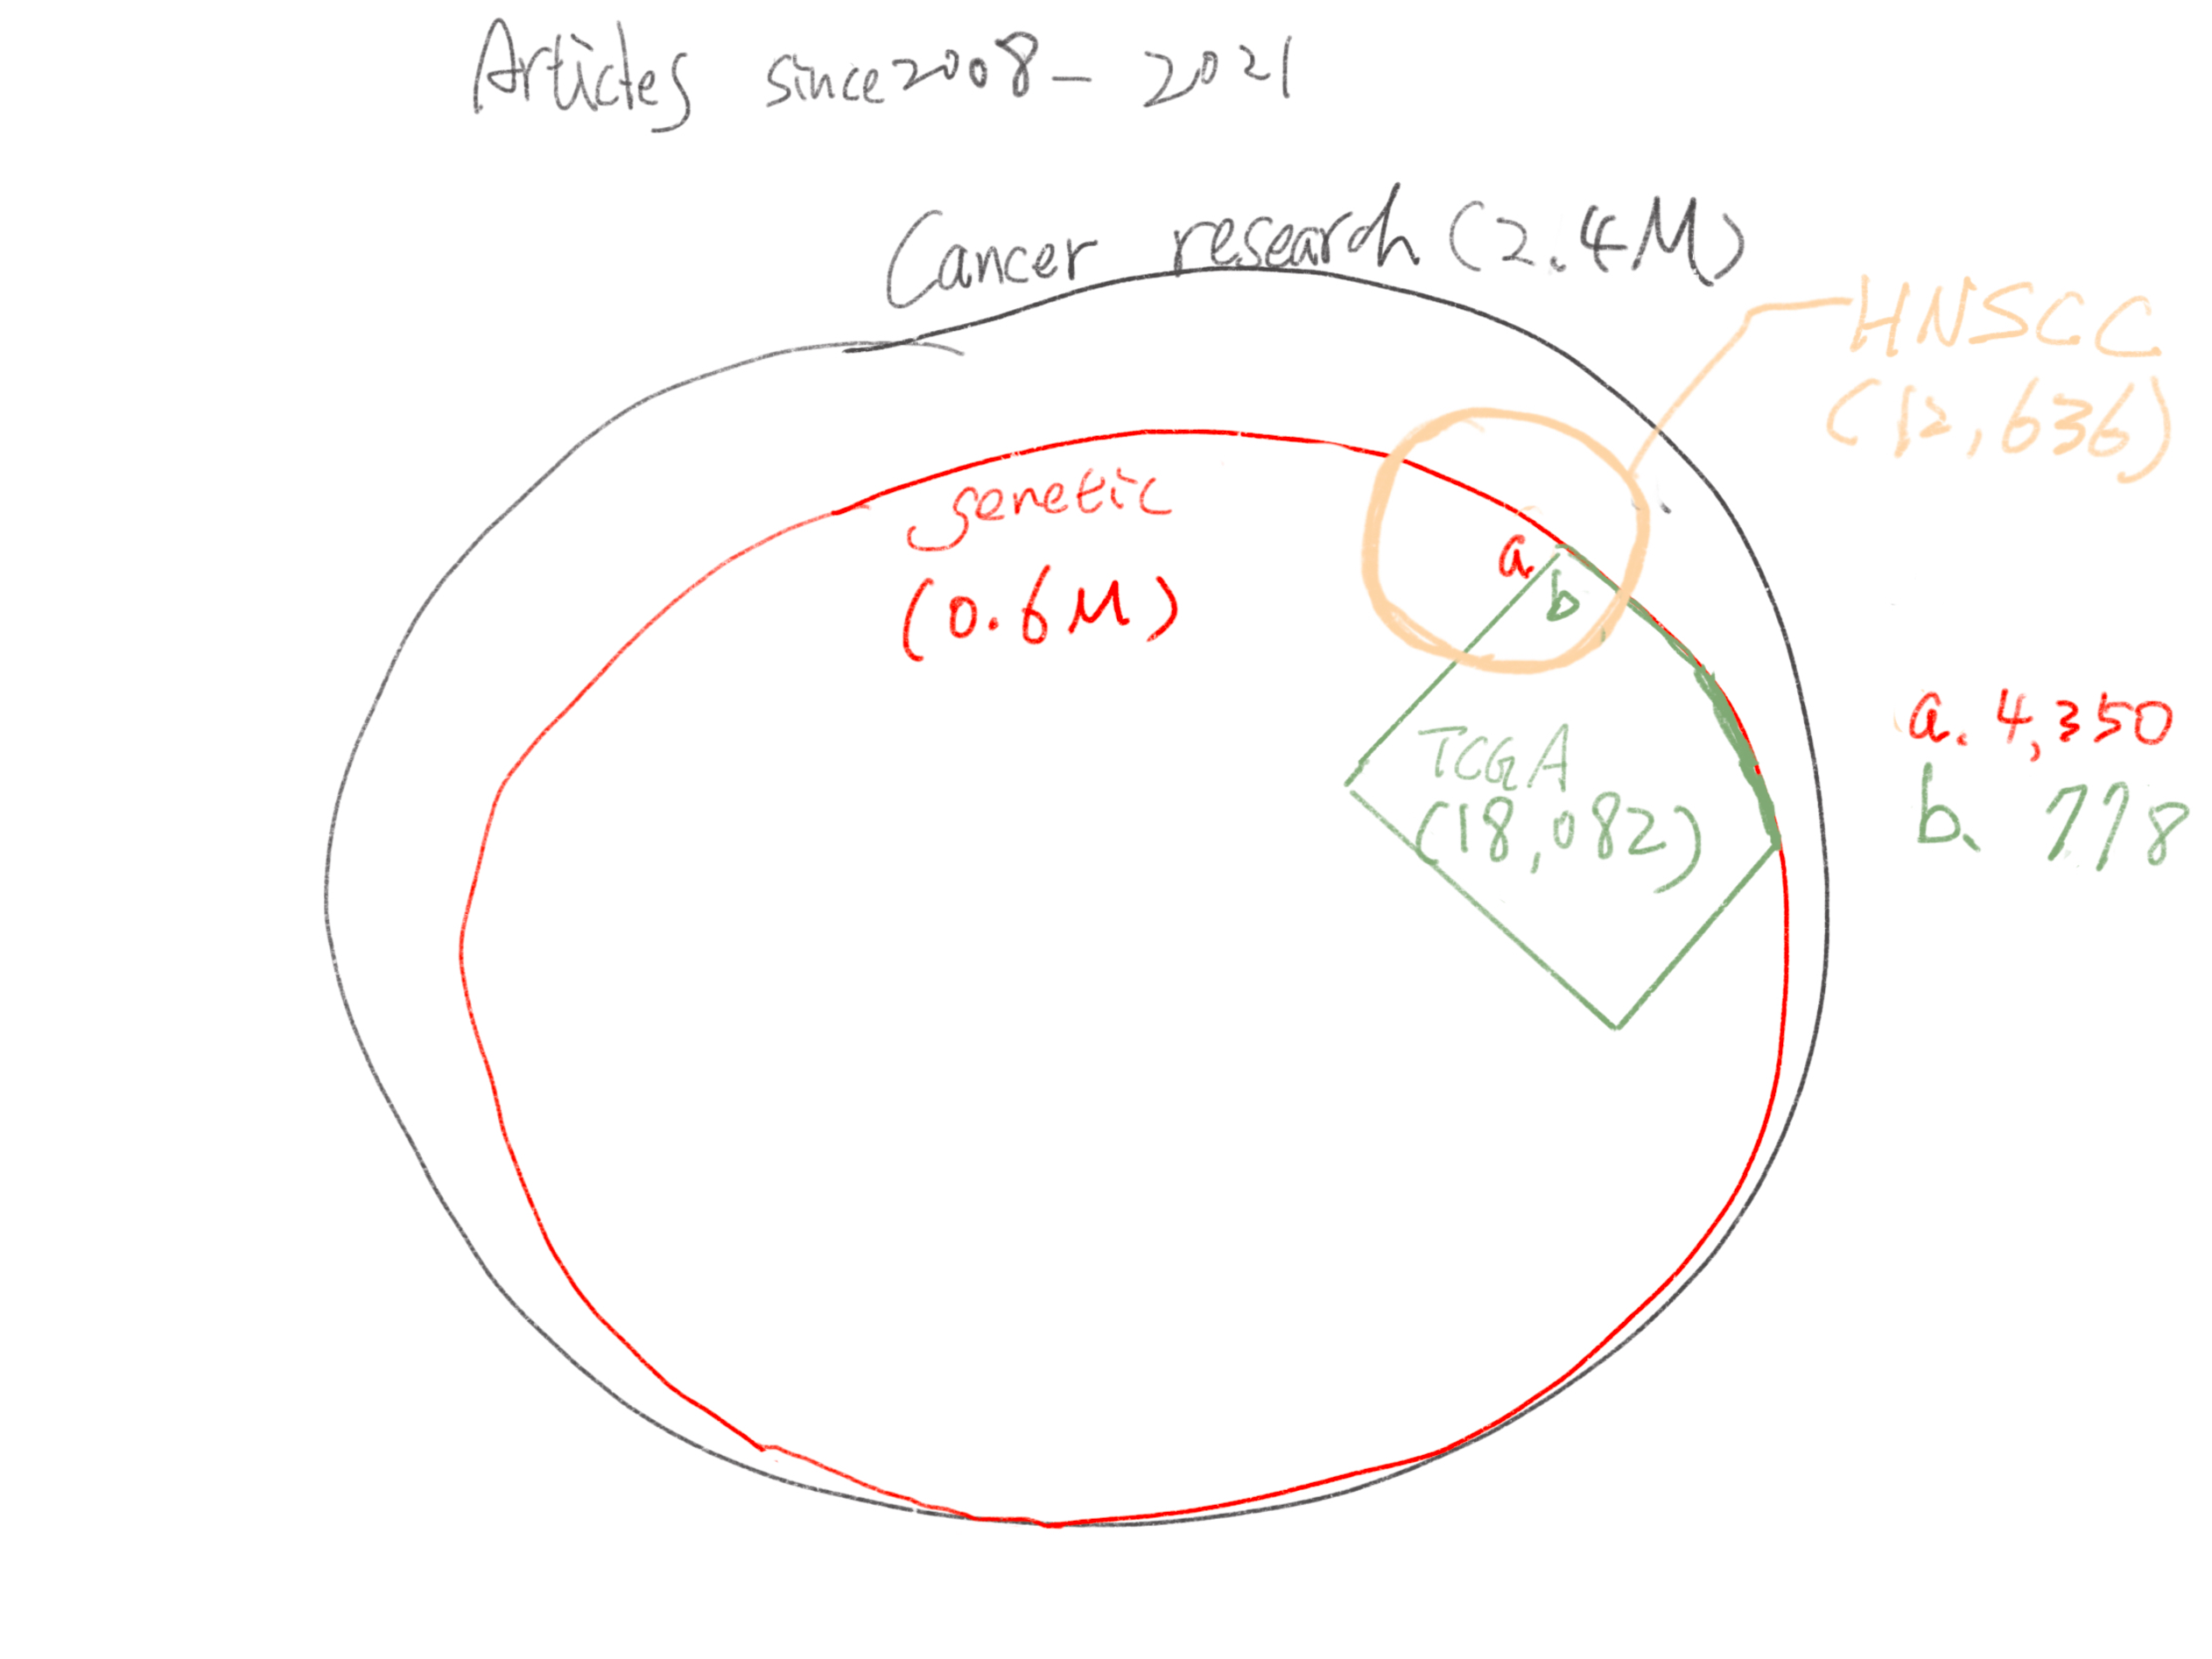
\includegraphics[width=14cm]{Answer_2-1.pdf}
\caption{Cancer research articles published from 2008 to 2021. Total: 2.4 million; genetic related: 0.6 million; HNSCC research: 12,636.}
\label{figure:fig_embase}
\end{figure}
\clearpage
%778/4350 = 17.9\% using TCGA data
%There is 374 genes in the oral cancer gene database of Indian HNSCC; http://www.bioinformation.net/006/97320630006169.pdf
%http://www.actrec.gov.in/OCDB/index.htm

Although other databases carrying HNSCC genomics and clinical data we found, such as MSKCC (151 cases), Broad (74 cases), Johns Hopkins (32 cases), MD Anderson (40 cases), and \acrshort{ncbi} Gene Expression Omnibus (GEO) datasets (e.x. GSE2837, 40 cases; GSE6631, 22 cases; GSE31056, 23 cases)\cite{Cerami2012b}\cite{Gao2013a}. However, the MSKCC, Broad, and Johns Hopkins databases were processed through whole-exome sequencing instead of whole-genome sequencing in the TCGA database.

There is several useful web-tools for survival analysis, such as cBioportal\cite{Cerami2012b}\cite{Gao2013a}, KM-Plotter\cite{Gyorffy2010},  SurvExpress\cite{Aguirre-Gamboa2013}, UALCAN (available at http://ualcan\\.path.uab.edu/)\cite{Chandrashekar2017a} and Gene Expression Profiling Interactive Analysis (GEPIA, GEPIA2)\cite{Tang2019}. According to the citing articles\cite{Wu2020} and their online documents, the back-end databases of those web-tools were collected from TCGA, the European Genome-phenome Archive (EGA)\cite{Lappalainen2015} and NCBI GEO datasets (available at https://www.ncbi.nlm.nih.gov/gds). Furthermore, almost all of their survival data came from the TCGA database.
%GEO (few survival features, less than 100 participate in each GSE dataset)
%GSE31056, GSE2837 (Prognoscan)
%there is survival feature: A total of 44 patients (22 HNSCC samples and 22 normal samples) were obtained from GSE6631
%有文章為證1. Lawrence, M. S. et al. Comprehensive genomic characterization of head and neck squamous cell carcinomas. Nature 517, 576–582 (2015).\cite{Lawrence2015a}
%datasets for each cancer type that include exactly the same prediction and outcome variables and consider comparable target populations. Currently, such data is simply not available.

%The Dickkopf1 (DKK1) gene encodes a protein that was mainly involved in Wnt and other signaling pathways.
%Inhibition of DKK1 in Hep-2 cells reduces their proliferation, colony formation, cell migration, and invasion in vitro\cite{Shi2014}.
%Pang et al\cite{Pang2018} demonstrated that upregulation of DKK1 in SBC-3 cells (human small cell lung cancer) enhanced their proliferation, colony formation, cell migration, and invasion in vitro, as well as bone metastasis in vivo. 
%Increased DKK1 levels in HNSCC tissues correlated with elevated VEGF-C and beta-catenin\cite{Shi2014}.
%DKK1 expression was significantly associated with smoking, alcohol abuse, sex, human papillomavirus status\cite{Chakraborty2020}, tumor site, tumor invasion, and pathologic stage in HNSCC patients.\cite{Gao2018}.
%The mRNA expression of DKK1 and DKK3 was elevated in human papillomavirus (HPV)-negative HNSCC\cite{Hu2020}.

For example, Wei et al.\cite{Wei2020} conducted the analysis of the prognostic value of DKK1 expression in human cancers based on bioinformatics tools, including UALCAN, GEPIA2 (dataset from TCGA)\cite{Tang2019}, and DriverDBv3 databases.
%using http://gepia2.cancer-pku.cn/detail.php?gene=DKK1 => \cite{Tang2019}
%GEPIA is a web-based tool that plots expression profiles of given genes (dataset from TCGA database)
They has suggested that overexpression of DKK1 indicates adverse OS in bladder urothelial carcinoma (BLCA)\cite{Wei2020}, HNSCC\cite{Chakraborty2020}\cite{Hu2020}\cite{Wei2020}, and pancreatic adenocarcinoma (PAAD)\cite{Wei2020}. %Moreover, DKK1 is increased in HPV\+ HNSCC leading to the worst prognosis of the patients. 
%\cite{Shi2014}\cite{Gao2018}\cite{Chakraborty2020}(non-TCGA)\cite{Hu2020}\cite{Wei2020}


Conclusion: TCGA database is representative of HNSCC.


\begin{figure}
\raggedleft
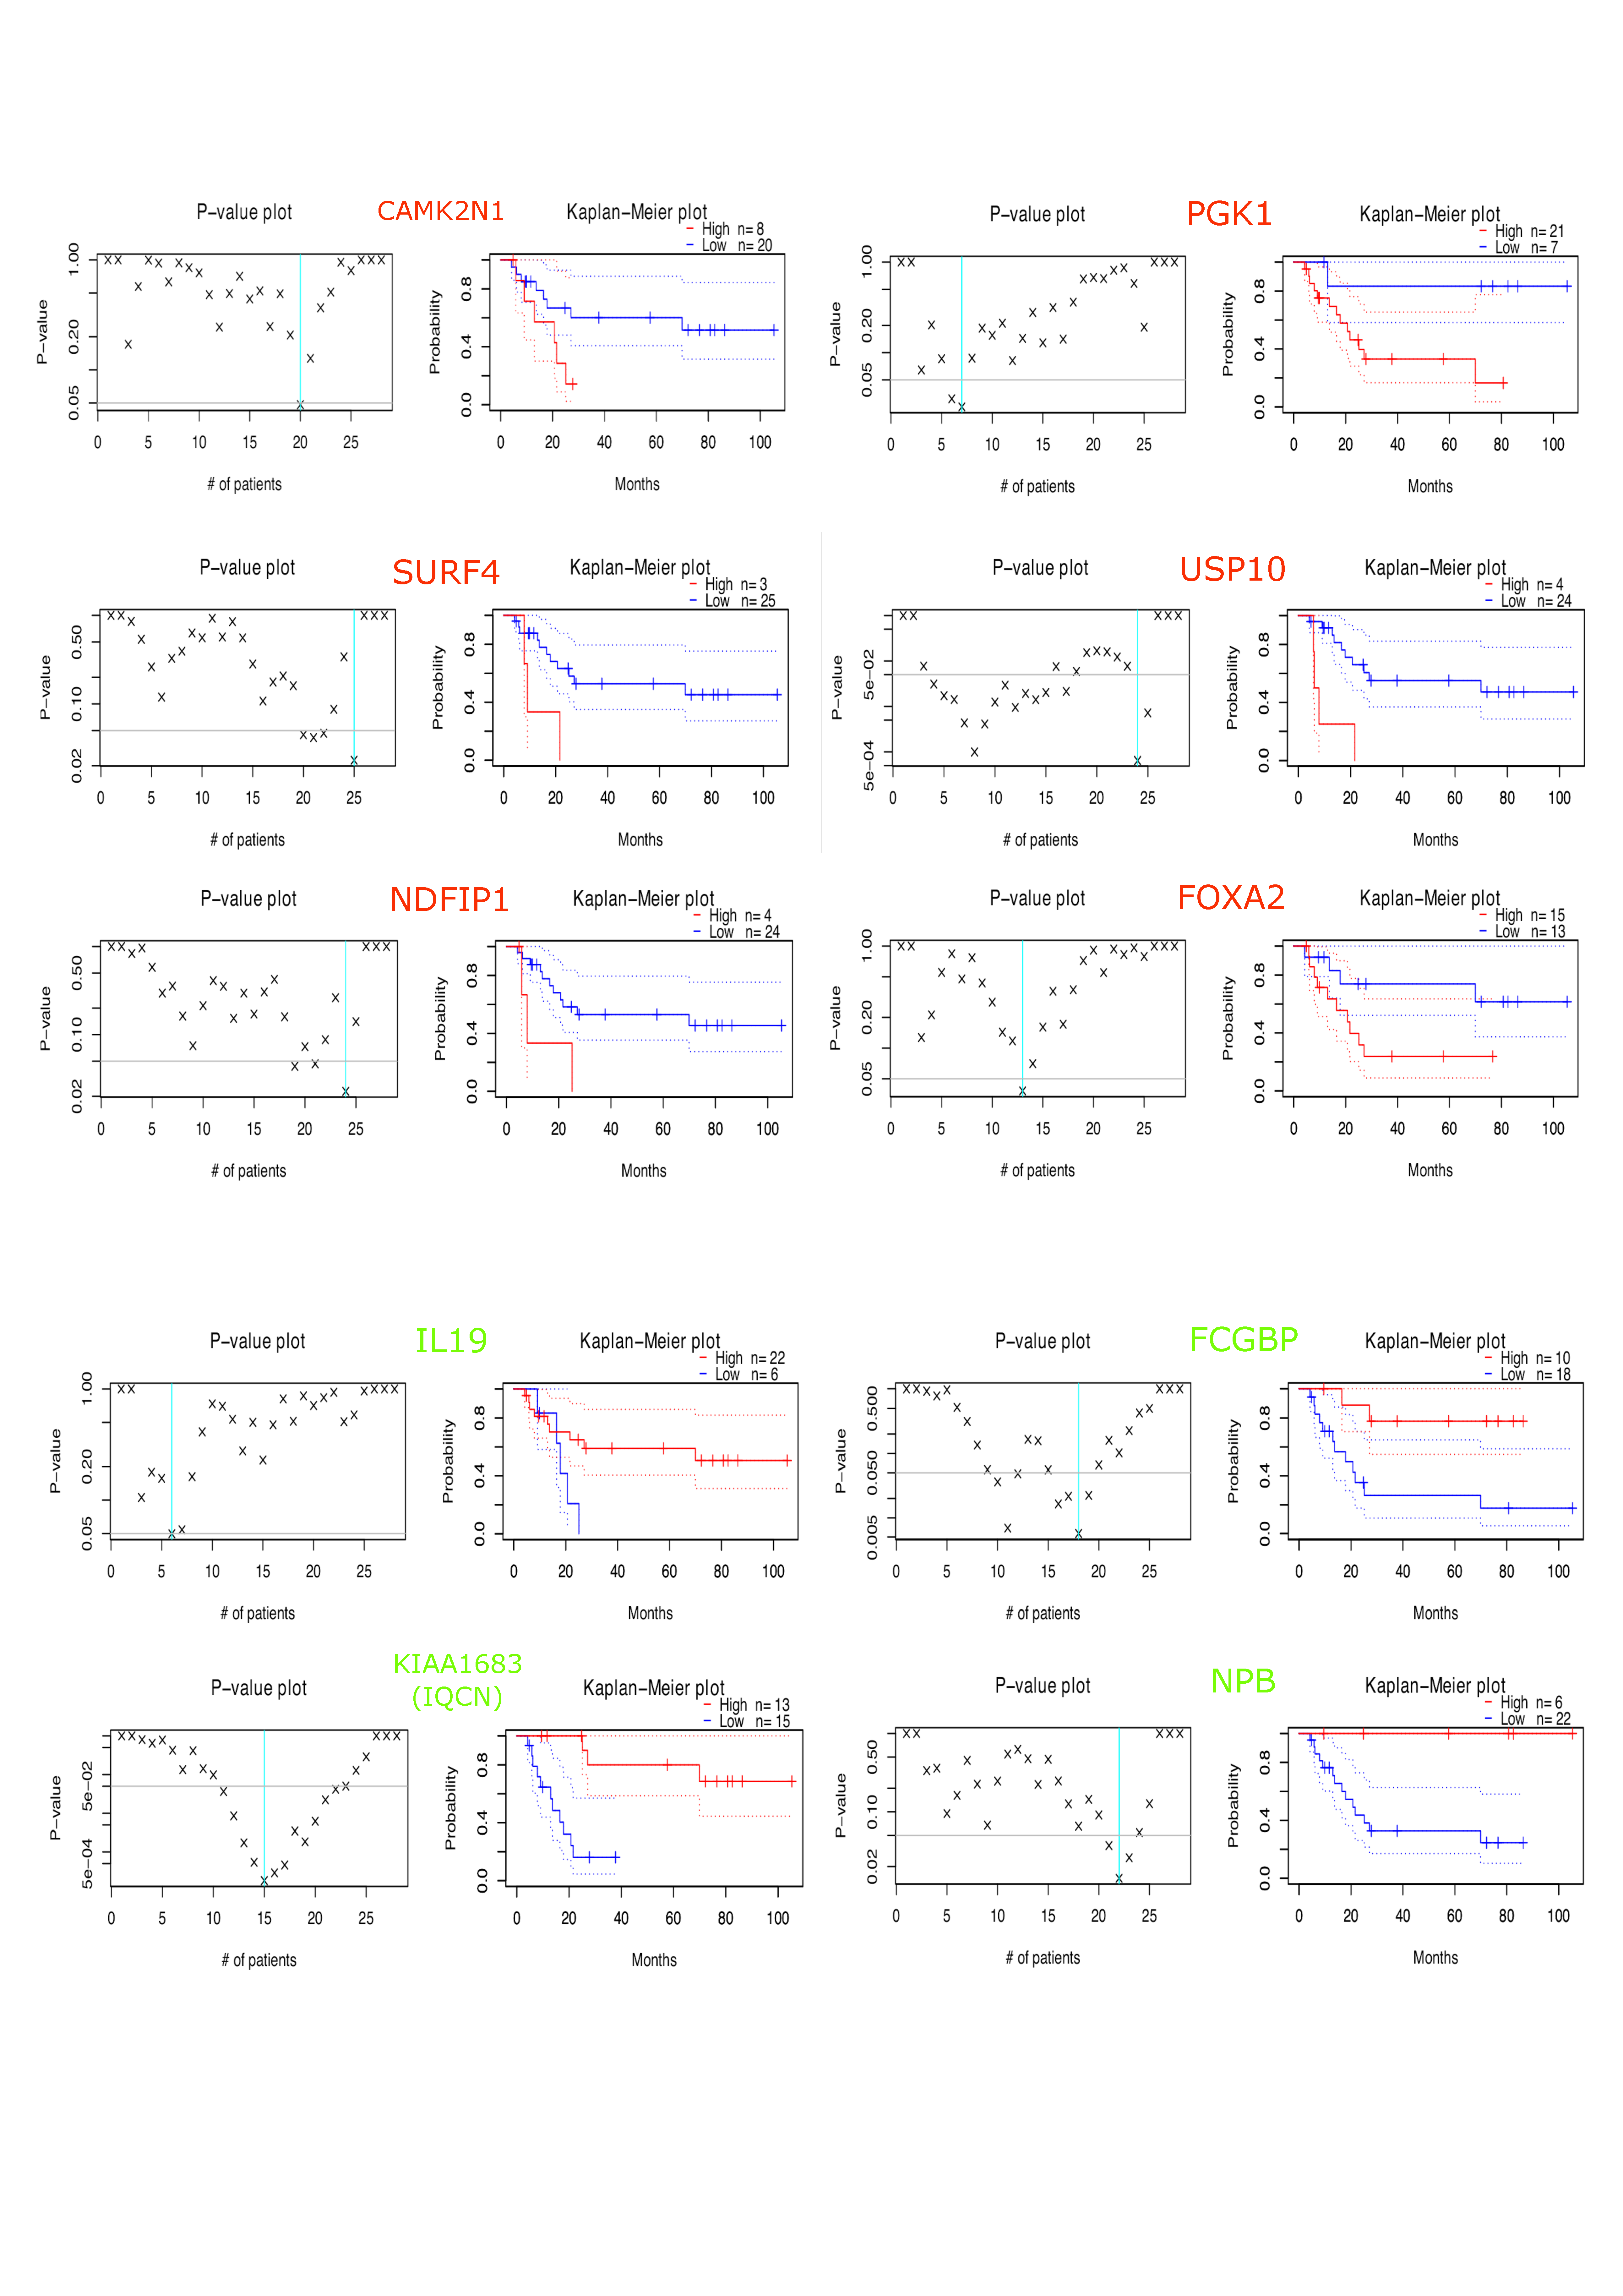
\includegraphics[width=14cm]{Answer_2-2.pdf}
\caption{GSE2837 query results from PrognoScan: Kaplan-Meier plots of 10 genes (the cutoff of \textcolor{red}{high risk} and \textcolor{blue}{low risk} groups, which is derived from cumulative P-value plots). The poor prognostic genes are marked as \textcolor{red}{red}; the better prognostic genes are marked as \textcolor{green}{green}.}
\label{figure:fig_GSE2837}
\end{figure}
\clearpage


%%%

% xxxxx
\begin{outline}
The data from TCGA database or other databases could be applied by this workflow, since modification of the R script is necessary to adapt the difference structure among datasets (e.x. data schema, table size, definition of features, number of features and their location on the table column).\\
In short, the elements of the workflow with the \{codes\} shows:\\
(please also see Figure \ref{fig:workflow})
\1 $[\# step 1 (main)]$
\{main\_marginSFP\_HNSCC.R\}
        \2 dataset retrieval from TCGA GDC data portal (in GDAC format)
%\1 $[\# step 1]$
    \2 \{TCGA\_HNSCC\_marginSFP.R\}
        \3 \underline{raw data cleaning}
        \3 \underline{data transformation and merge}
        \3 \underline{dichotomization of clinical features}
%     \item Using a serial cut from 30\% to 70\% percentile of the cohort, it could find the least P-value cutoff of the Kaplan-Meier analysis for each gene expression.
        \3 survival analysis
            \4 cut off finder by \{cutofFinder\_func\_HNSCC.R\}
%     \item The R script program could automatically scan protein-coding genes and generate the Kaplan-Meier plots and Cox's univariate/multivariate tables.
            \4 Cox modelling
\1 $[\# step 2]$
\{analysis\_export.R\}
    \2 analysis of the tables generated from \# step 1
    \2 candidate selection
%    \item Our analysis could discover the pronounced biomarkers, which impact HNSCC's survival under the stringent Bonferroni adjustment.
\1 (remark: only the \underline{underlined} portion in \{TCGA\_HNSCC\_marginSFP.R\} should be re-coded aggressively)
\end{outline}

%\begin{outline}
%\linebreak

%\1 $[\# step 1]$
%\{TCGA\_HNSCC\_marginSFP.R\}
%    \2 raw data cleaning
%    \2 data transformation and merge
%    \2 clinical features
%\end{itemize}
%\end{outline}


%to generalize the utility of our workflow:
%R scripts could be re-coded and applied to start a new analysis of dataset.
% *** R 的特色 邊分析解讀,一邊 coding
%Currently, less HNSCC dataset is available worldwide (Indian?) => 
%能否套用在別的 database,可以,需要標準化(fpkm or RSEM)
%It made the messenger \acrshort{rnaseq} matrix with log2 transformed for the downstream analysis, as described in their reference\cite{RSEM2016}.?)

%Moreover, we are planning to extend this workflow applied to other studies, such as TCGA CRC (colorectal cancer), TCGA LUAD (lung adenocarcinoma), or TCGA BRCA (breast cancer).
%Then it is possible to introduce the Rstudio Shiny app (https://shiny.rstudio.com) as a web application of the "pvalueTex" packaged with our workflow in the future.


%(other cancer types in the TCGA database). 
%TCGA HNSCC -> TCGA CRC, TCGA LUAD, TCGA BRCA cohorts -> GEO or other uploaded cancer cohort

% workflow from the manuscript ##########
%The number of protein-coding genes was suggested as 20,500\cite{Clamp2007}. The \acrshort{gdc} Data Portal provided \acrshort{tcga} data has been harmonized and re-aligned \acrlong{rnaseq} data against an official reference genome build (\acrlong{grch38}, \acrshort{grch38}). \acrshort{rnaseq} expression level read counts produced by Illumina HiSeq have been normalized using the \acrfull{fpkm} method, as described in reference\cite{FPKM2017}.
%The \acrshort{rnaseq} preprocessor of Broad \acrshort{gdac} picked the \acrfull{rsem} value from Illumina HiSeq/GA2 messenger \acrshort{rnaseq} level\_3 (v2) dataset of \acrshort{nci} \acrshort{gdc}. It made the messenger \acrshort{rnaseq} matrix with log2 transformed for the downstream analysis, as described in their reference\cite{RSEM2016}.
%We utilized FirebrowseR's function call, Samples.mRNASeq(cohort = "HNSC", gene=GeneName, format="csv"), to download each \acrshort{rnaseq} data of all \acrshort{hnscc} patients and to save as 20,499 data frame files, named as "HNSCC.mRNA.Exp.[GeneName].\newline
%Fire.Rda".
%After careful investigation of the genomics dataset, the \acrshort{rnaseq} values of "\acrfull{slca}" and "\acrfull{slcb}" should be considered two distinct expression entities. We concluded that the number of protein-coding genes in the \acrshort{tcga} dataset is 20,500. We removed null expressed genes, which over 50\% of the cohort, to avoid the useless result.

%We utilized FirebrowseR's function call, Samples.Clinical(cohort = "HNSC", format="csv"), to get all 81 clinical features (including pathological data, defined by \acrshort{tcga} \acrshort{gdc} data dictionary: \acrfull{cde}\cite{CDE2019}) of all 528 \acrshort{hnscc} patients, which saved as one data frame file: "HNSCC.clinical.\linebreak
%Fire.Rda" (accessed November 2019).

%One "HNSCC.clinical.Fire.Rda" tables and 20,500 "HNSCC.mRNA.Exp.\newline
%[GeneName].Fire.Rda" tables were transposed and merged by their \newline
%\_participant\_barcode (unique patient \acrlong{id}, \acrshort{id}) to yield a data frame with 528 rows (participants) against 20,581 columns (81 clinical features as well as 20,500 protein-coding \acrshort{rnaseq} of cancer specimen).
%The clinicopathological features selected for our workflow included gender, age, clinical tumor size, clinical cervical lymph node metastases, clinical distant metastasis assessment, pathological surgical margin, and tobacco exposure with their corresponding survival data.
%The tumor size (T), cervical lymph node metastases (N), and distal metastasis status (M) were classified according to \acrfull{ajcc}\cite{Amin2017} along with \acrfull{uicc}\cite{Brierley2016} \acrshort{tnm} system for clinical staging of \acrshort{hnscc}.
% In the Eighth Edition, the AJCC has expanded the use of non-anatomic prognostic factors and biomarkers in assigning prognostic stage groups.
%%We made data clean by removing duplicated rows and columns.


%\subsection{Cutoff Finder Core Engine}
%To evaluate the effect of gene expression on the patient's survival, we introduced the stratifying of patients with Kaplan-Meier survival analysis according to each gene's low/high expression.
%Our cutofFinder\_func subroutine employs the minimum P-value approach to recognizing cutoff points in continuous gene expression measurement for patients sub-population.
%First, patients were ordered by \acrshort{rnaseq} value (RSEM) of a given gene. Next, patients were stratified at a serial cut (counted by person ranked in 30\% to 70\% percentile of the cohort; please see Figure \ref{fig:figure1} "HNSCC cohort"). The survival risk differences of the two groups were estimated by log-rank test to yield around 165 Kaplan-Meier P-values for each gene.
%Then, the optimal cutoff of \acrshort{rnaseq}, giving the minimum P-value, was selected by the cutofFinder\_func subroutine.
%This iteration method could calculate all possible cutoff of each gene expression in this cohort. At each run of cutofFinder\_func function call for an individual gene, it returned an optimal cutoff value (e.x. 0.027 for gene \acrlong{CAMK2N1}, \acrshort{CAMK2N1}). The optimal cutoff value and its correlated patient grouping size (e.x. low-expression in 262 persons vs. high-expression in 152 persons with gene \acrshort{CAMK2N1}) would be returned to the main program to allow downstream Cox survival analysis. The percentile range we applied as 30\% to 70\% was used to avoid a small grouping effect\cite{Miller1982}\cite{Mizuno2009a}.
%In case there was no significant P-value, a median expression of this gene was set as its cutpoint as usual.


%\subsection{Biomarker Selection}

%Those genes with prognostic impact, whose hazard ratio $>=1.5$ or $<=0.5$ in both Cox's univariate/multivariate model, were assigned as provisional candidates.
%Bonferroni adjusted (Kaplan-Meier) P-value was used to make a ranking of candidates for the final decision (see Figure \ref{fig:figure1}, step 2).



% we plan to extend this workflow on other TCGA cancer types
%Our strategy still has the strength to explore the more possible biomarkers from \acrshort{rnaseq} datasets in cancer research.
% second limitation:
%In line with tumor-agnostic research, we plan to explore more TCGA diseases to find common biomarkers. However, the \acrshort{gdc} provided standardized data frames that could not directly fit our workflow's scope. Before the global genes scanning process, we needed to re-format, transpose and, merge the 528 patients' clinical datasets and correlated 20,500 expressions of bio-specimen. It should be carefully curated to confirm the data integrity with the correct definition. We also plan to upgrade our plain R script at the Rstudio platform to program in the C++ language and source it in R. The high performance of C++ could speed up the cutoff finding engine in this workflow involving heavy computations\cite{Woodward2020}. Thus, it is possible to introduce the Rstudio Shiny app (https://shiny.rstudio.com) as a web application of the "pvalueTex" packaged with our workflow in the future.
%\end{MyColorPar}
